\documentclass[a4paper]{article}

\usepackage[utf8]{inputenc}
\usepackage[T1]{fontenc}
\usepackage{textcomp}
\usepackage[UKenglish]{babel}
\usepackage{amsmath, amssymb}
\usepackage{subcaption}
\usepackage{listings}
\usepackage{float}

\setlength{\parindent}{0pt}
\setlength{\parskip}{1em}

\lstset{breaklines=true}
% figure support
\usepackage{import}
\usepackage{xifthen}
\pdfminorversion=7
\usepackage{pdfpages}
\usepackage{transparent}
\newcommand{\incfig}[1]{%
	\def\svgwidth{\columnwidth}
	\import{./figures/}{#1.pdf_tex}
}

\pdfsuppresswarningpagegroup=1

\begin{document}
	\section{Part 1: Thresholding}
	\subsection{Introduction}
	Thresholding is a technique used to segment an image based on grey level
	intensities within the image. Two common methods of thresholding an
	image are applying a "Fixed Global Threshold" and applying an "Adaptive
	Threshold". Each of these methods take a greyscale input image, and
	output a binary (black and white) image.
	\par Fixed Global thresholding involves applying a single threshold value
	across the image, i.e. if the intensity value of the pixel is greater
	than the threshold value, set that pixel to white, otherwise, set it to
	black.
	\par Adaptive thresholding techniques base their threshold values at the
	current pixel off the neighbouring pixels. The "5x5 Adaptive
	Thresholding" method utilised in this section takes the mean intensity
	value of the 24 pixels surrounding the currently selected pixel as the
	threshold value for the currently selected pixel. If this center pixels
	intensity value is greater than the threshold, it's value is set to
	white, otherwise it is set to black.
	\subsection{Techniques}
	A number of techniques are used in the completion of this assignment. As
	such each technique will only be introduced once, on it's first use. In
	completing this section of the assignment, the following techniques
	are utilised:
	\subsubsection{Part a}
	\underline{\textbf{Load Image}}
	\par Matlabs ``imread()'' function is used to load an image, whose filename
	is passed as an argument to the function, as an array in the form
	$X \times Y \times 3$ where X and Y are the dimensions of the image, and
	the ``3'' represents the colour channels (RGB).
	\par \underline{\textbf{Colour to Greyscale}}
	\par The Matlab ``rgb2gray()'' function converts a colour image to a
	greyscale image. The three channel RGB image is converted to a single
	channel greyscale image based on the luminance of each pixel in the
	image. The output single channel values range from $0-255$.
	\par\underline{\textbf{Show Image}}
	\par The Matlab ``imshow()'' function is used to display an image on
	screen.
	\subsubsection{Part b}
	\underline{\textbf{Threshold}}
	\par The VSG ``Threshold'' function applies a fixed global threshold to
	the input image. If the pixel value is less than the threshold value,
	the pixel is set to black, otherwise it is set to white.
	\subsubsection{Part c}
	\underline{\textbf{5x5 Threshold}}
	\par The VSG ``5x5Thresh'' function applies an adaptive 5x5 threshold
	to the image. The function defaults to a threshold offset of value zero.
	\par When the value of the center pixel in the 5x5 region is less than the
	mean of the 5x5 region minus the offset, the pixel is set to black,
	otherwise it is set to white.
	\subsubsection{Part d}
	\underline{\textbf{Gaussian Noise}}
	\par The Matlab ``imnoise()'' function, when used with the `gaussian' input
	parameter, applies Gaussian noise with mean specified by input
	parameter `m', and variance `var', e.g:
	\begin{lstlisting}
	imnoise(img1, 'gaussian', 0, var)
	\end{lstlisting}
	The above example applies zero-mean Gaussian noise to the image
	``img1'', with a variance ``var''.
	\subsection{Pseudocode}
	\subsubsection{Part a}
	\begin{enumerate}
		\item Load the image into Matlab using the ``imread()''
			function
		\item Use the ``rgb2gray()'' function to convert the image to
			greyscale.
		\item Display the greyscale image using the ``imshow()''
			function.
	\end{enumerate}
	\subsubsection{Part b}
	\begin{enumerate}
		\item Follow the steps of Part a.
		\item Apply a fixed global threshold using the VSG package
			``Threshold'' function. An arbitrary value should be
			chosen for the fixed threshold value.
		\item Vary the fixed threshold value in order to obtain optimal
			background/foreground segmentation, while retaining
			facial features.
		\item Display the thresholded images using the ``imshow()''
			function.
	\end{enumerate}
	\subsubsection{Part c}
	\begin{enumerate}
		\item Follow the steps of Part a.
		\item Apply a 5x5 adaptive threshold using the VSG package
			"5x5Thresh" function.
		\item Display the adaptive thresholded image using the
			``imshow()'' function.
	\end{enumerate}
	\subsubsection{Part d}
	\begin{enumerate}
		\item Follow the steps of Part a.
		\item Apply Gaussian noise to the greyscale image using the MIP
			``imnoise()'' function. Zero-mean noise should be used
			for this section.
		\item Execute the fixed global thresholding and 5x5 adaptive
			thresholding procedures as described in part b and part
			c respectively.
		\item Adjust the variance value of the ``imnoise()'' function.
			Repeat steps 2 and 3.
	\end{enumerate}
	\subsection{Results}
	\subsubsection{Part a}
	The image is correctly loaded into Matlab, converted to greyscale, and
	displayed. The input image is of dimensions $512\times 348\times 3$, and
	is of data type integer. This means that the image is in the RGB colour
	space, with the red, green, and blue channels represented by a value of
	0-255 for each pixel in the image. The resulting greyscale image is of
	dimensions  $512\times 384$ and is also of type integer. The single
	channel representing the greyscale intensities have values ranging from
	0-255.
	\begin{figure}[H]
		\centering
		\subcaptionbox{Input Image}
		[.5\linewidth]{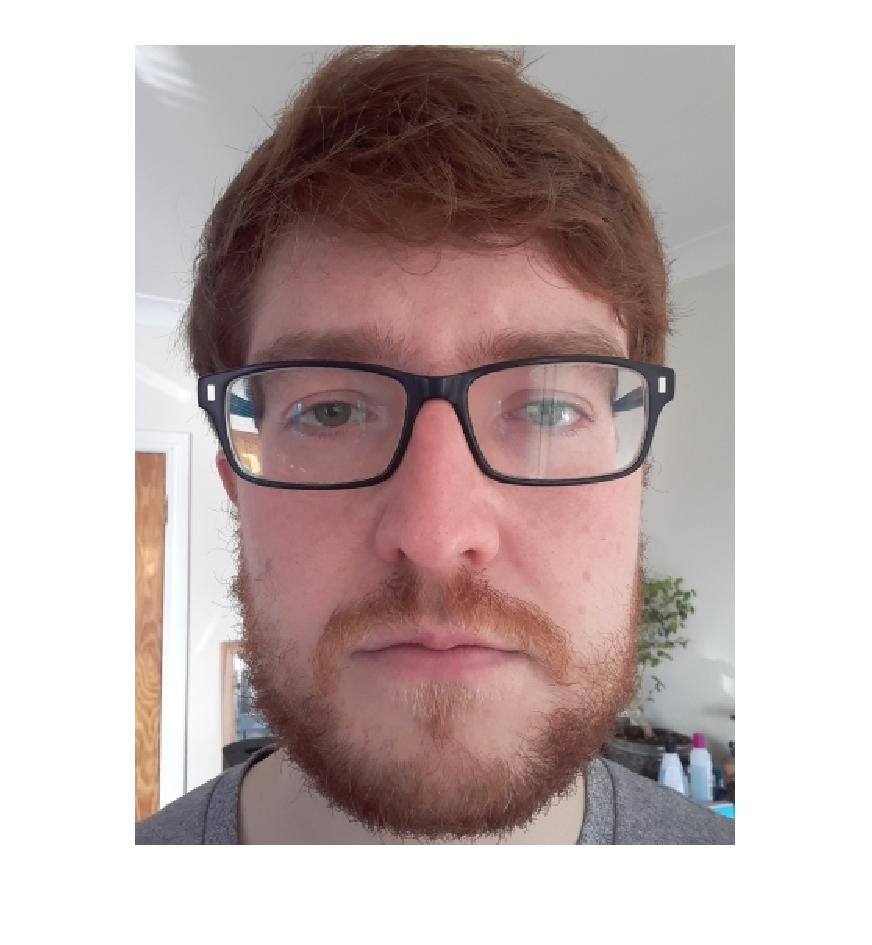
\includegraphics[height=5cm]{Results/Q1/a/qaInput.jpg}}%
		\subcaptionbox{Greyscale Image}
		[.5\linewidth]{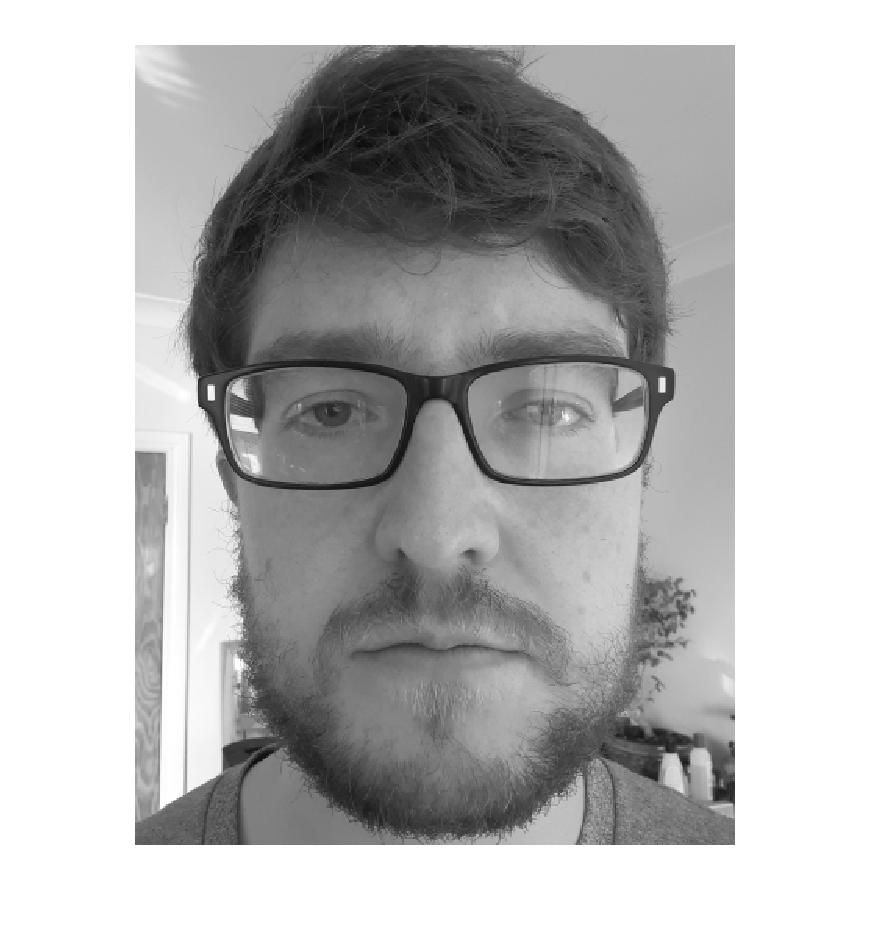
\includegraphics[height=5cm]{Results/Q1/a/qaGreyscale.jpg}}%
		\caption{Input and Greyscale Images}
		\label{fig:}
	\end{figure}
	\subsubsection{Part b}
	The VSG ``Threshold'' function is applied, with varying threshold
	values, to the input greyscale image. The ``Threshold'' function returns
	images with the same dimensions as the input image, however the data
	type returned is ``double'' rather than ``integer''. The initial value of the
	threshold is 199, calculated by taking $\frac{3}{4} \times (Higghest
	Grey Intensity + Lowest Grey Intensity)$.As this threshold does not
	provide adequate separation of the features in the image, arbitrary
	values of 125, 130, and 140 are also used. The image thresholded at 125
	has the greatest level of separation between the face and background,
	while also retaining as much detail as possible in the facial features.
	\begin{figure}[H]
		\centering
		\subcaptionbox{Data Driven Threshold}
		[.5\linewidth]{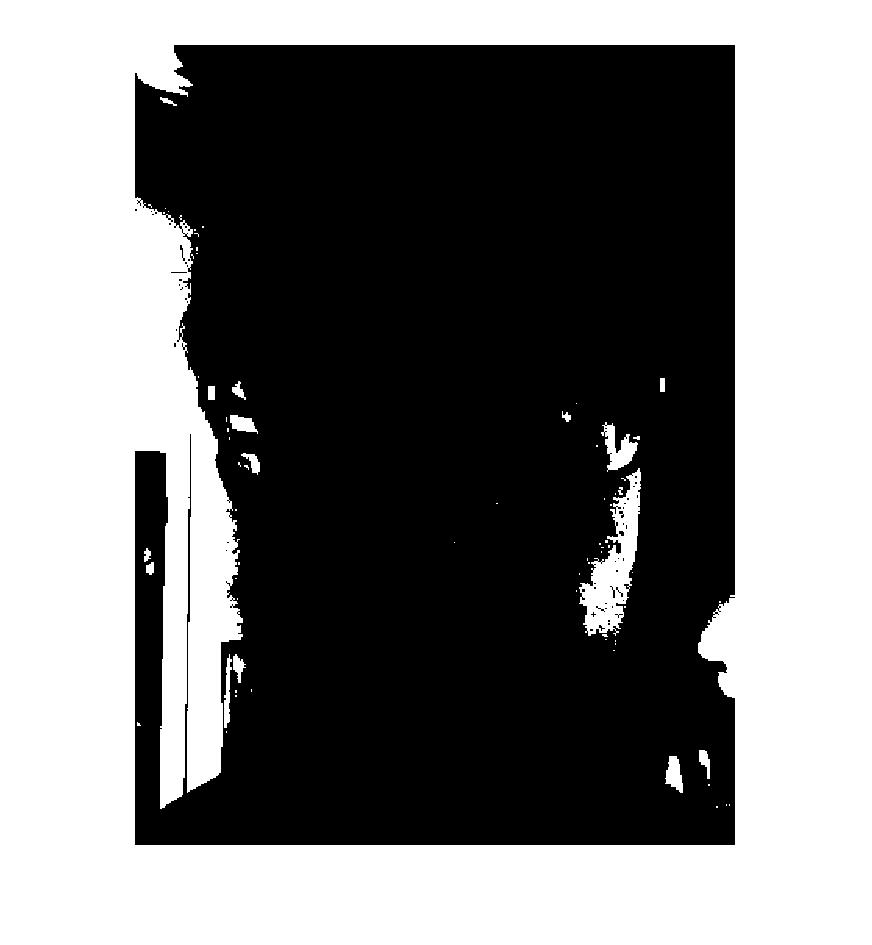
\includegraphics[height=5cm]{Results/Q1/b/qbThreshData.jpg}}%
		\subcaptionbox{Threshold$=125$}
		[.5\linewidth]{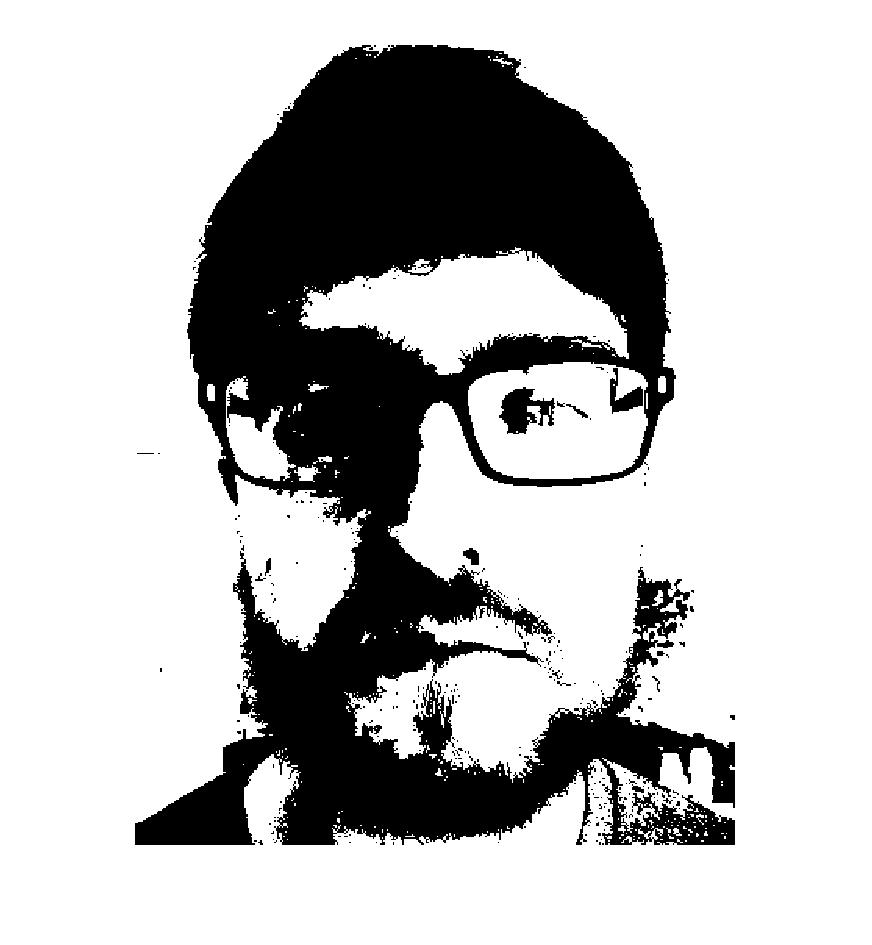
\includegraphics[height=5cm]{Results/Q1/b/qbThresh125.jpg}}%
		\caption{``Threshold'' Function Output}
		\label{fig:}
	\end{figure}
	\begin{figure}[H]
		\centering
		\subcaptionbox{Threshold$=130$}
		[.5\linewidth]{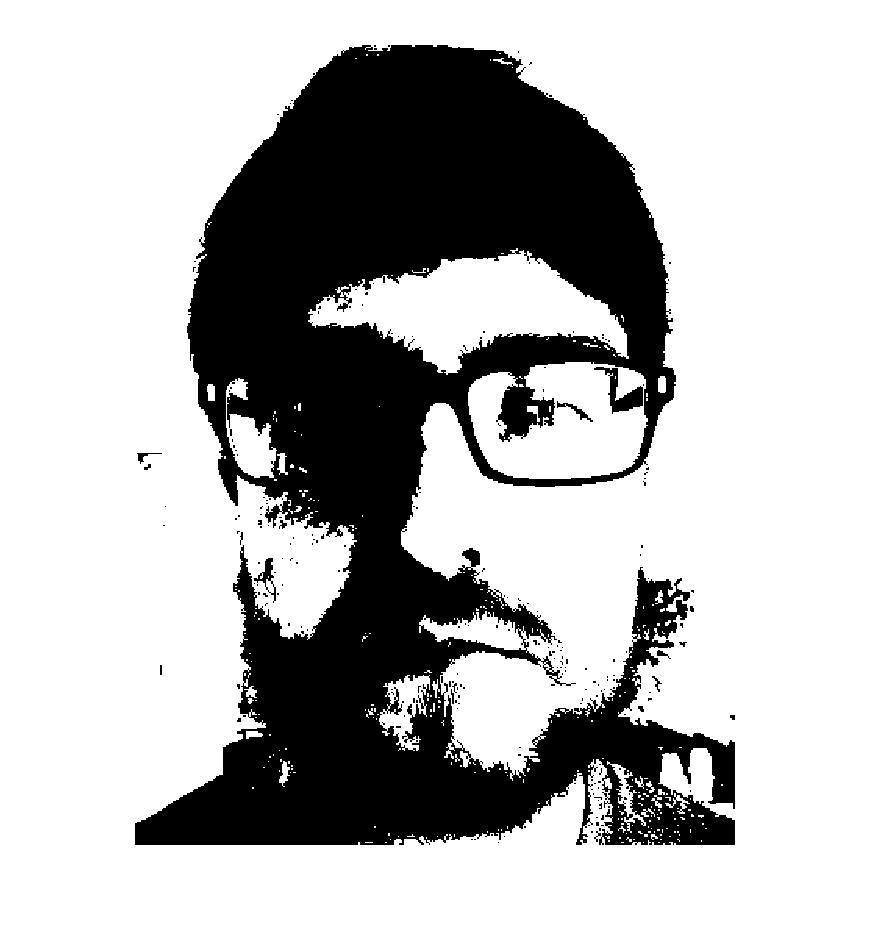
\includegraphics[height=5cm]{Results/Q1/b/qbThresh130.jpg}}%
		\subcaptionbox{Threshold$=140$}
		[.5\linewidth]{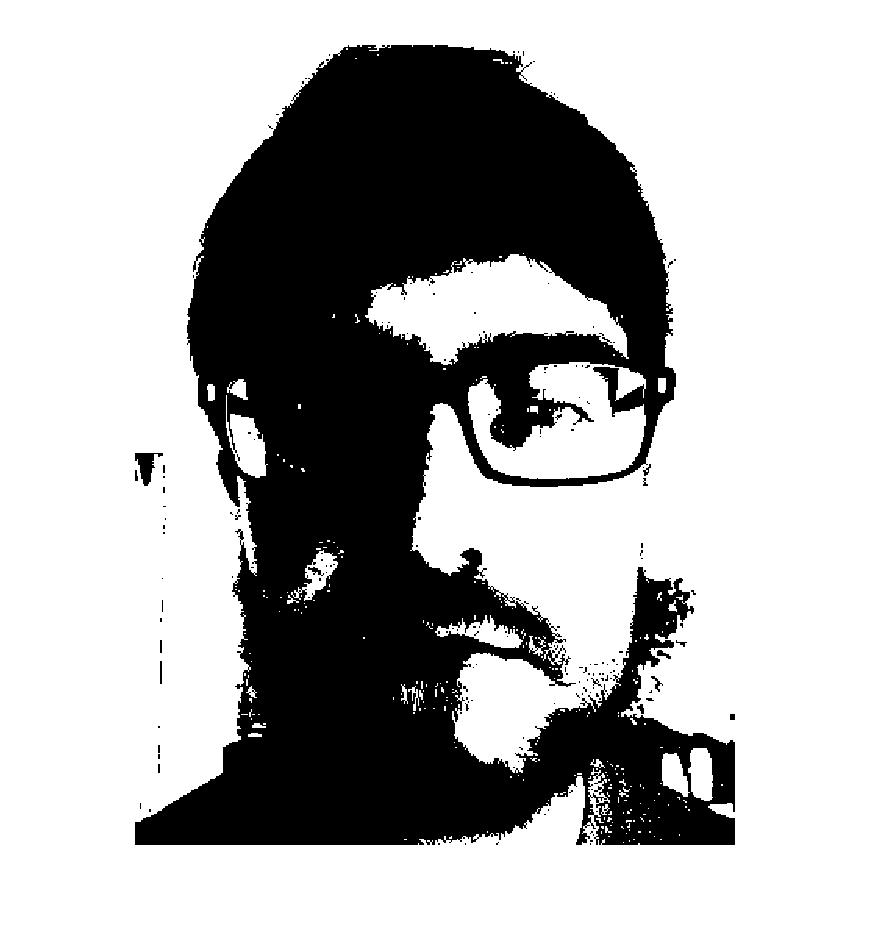
\includegraphics[height=5cm]{Results/Q1/b/qbThresh140.jpg}}%
		\caption{``Threshold'' Function Output}
		\label{fig:}
	\end{figure}
	\subsubsection{Part c}
	The VSG ``5x5Thresh'' function is applied to the input greyscale image.
	The resulting image is of type ``double'' and has the same dimensions as
	the input image. When compared with the fixed global threshold images,
	there is much greater separation of the foreground from the background,
	with all of the facial features fully visible. Features which are
	thresholded out due to lighting conditions in the fixed global threshold
	are retained here, such as the eyes.
	\begin{figure}[H]
		\centering
		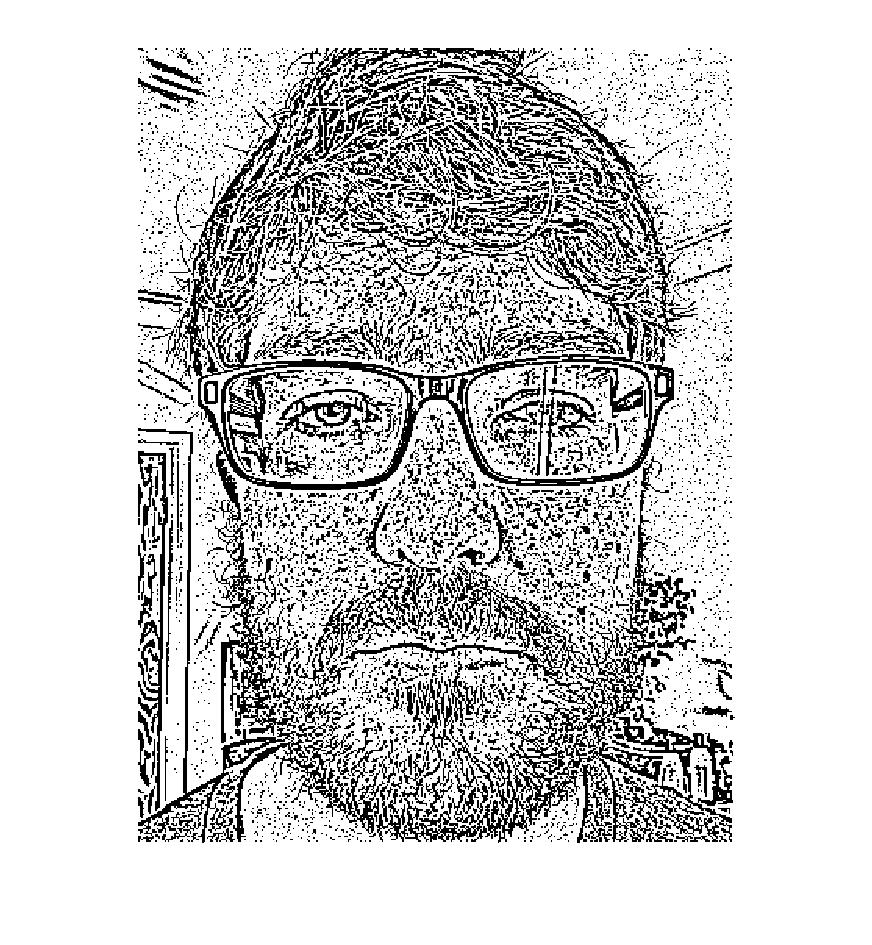
\includegraphics[height=5cm]{Results/Q1/c/qcThresh5x5.jpg}%
		\caption{``5x5Thresh'' Function Output}
		\label{fig:}
	\end{figure}
	\subsubsection{Part d}
	Gaussian noise is added to the greyscale image, and the ``Threshold''
	and ``5x5Thresh'' functions are applied. As can be observed from the
	images, the fixed global threshold is less sensitive to noise. This is
	due to the 5x5 Threshold using the average value of an area of pixels to
	set the threshold value. As such, noise within an area can skew the
	result of the thresholding, making this function much more sensitive
	to noise.
	\begin{figure}[H]
		\centering
		\subcaptionbox{Noisy Image}
		[.3\linewidth]{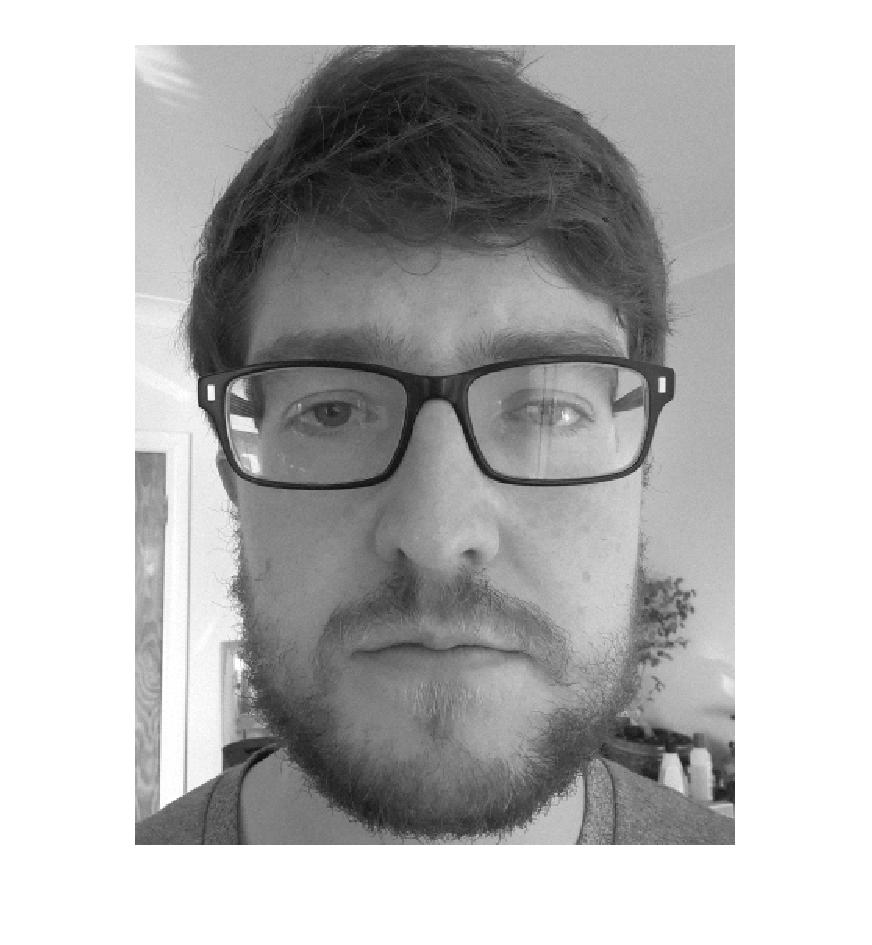
\includegraphics[height=5cm]{Results/Q1/d/qdVar00001.jpg}}%
		\subcaptionbox{Global Threshold}
		[.3\linewidth]{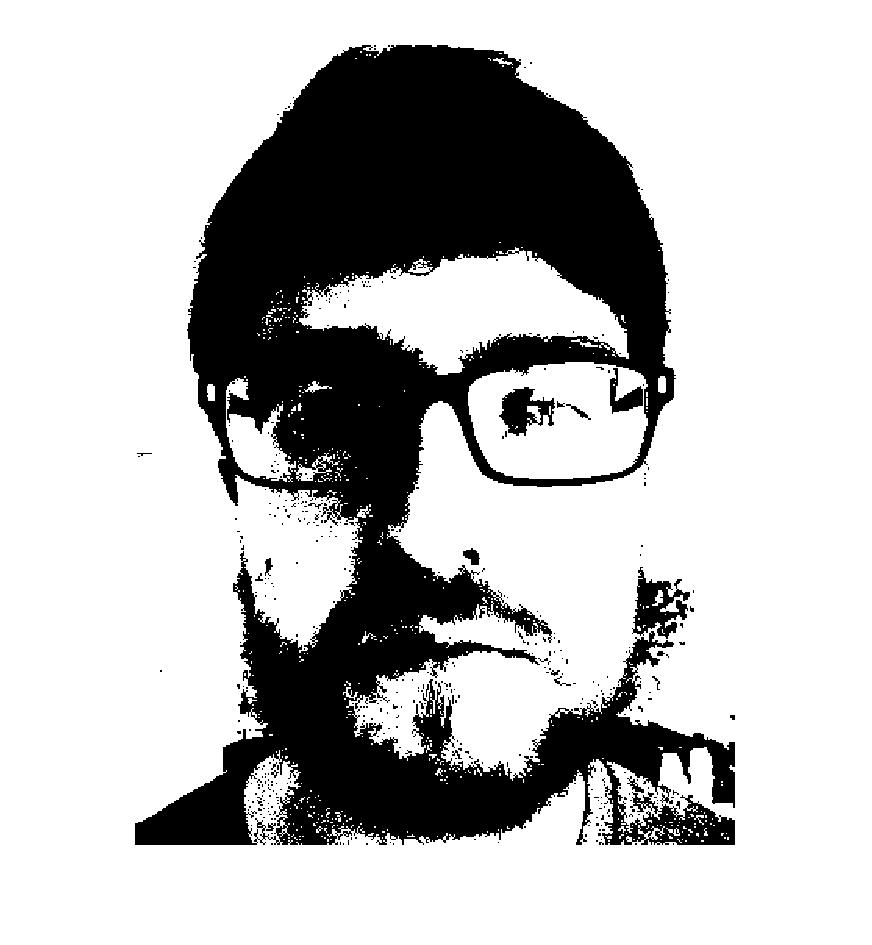
\includegraphics[height=5cm]{Results/Q1/d/qdThresh00001.jpg}}%
		\subcaptionbox{5x5 Threshold}
		[.3\linewidth]{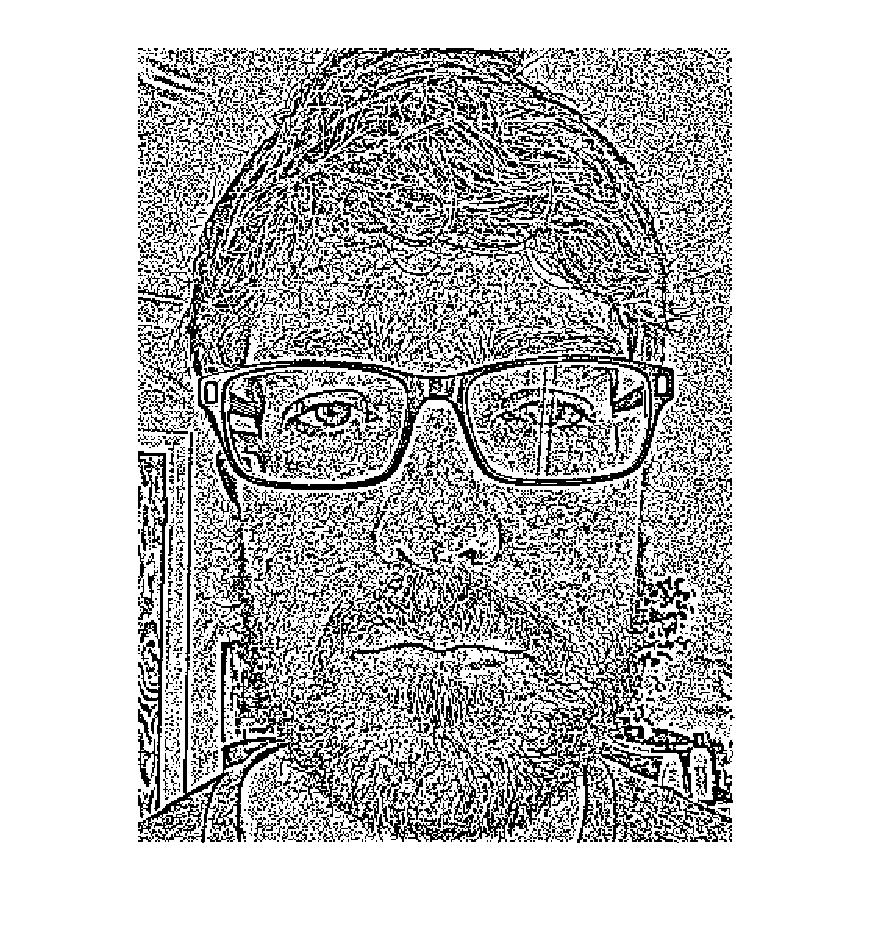
\includegraphics[height=5cm]{Results/Q1/d/qd5x500001.jpg}}%
		\caption{Thresholded Images after Gaussian Noise (0.0001
		Variance)}
		\label{fig:}
	\end{figure}
	\begin{figure}[H]
		\centering
		\subcaptionbox{Noisy Image}
		[.3\linewidth]{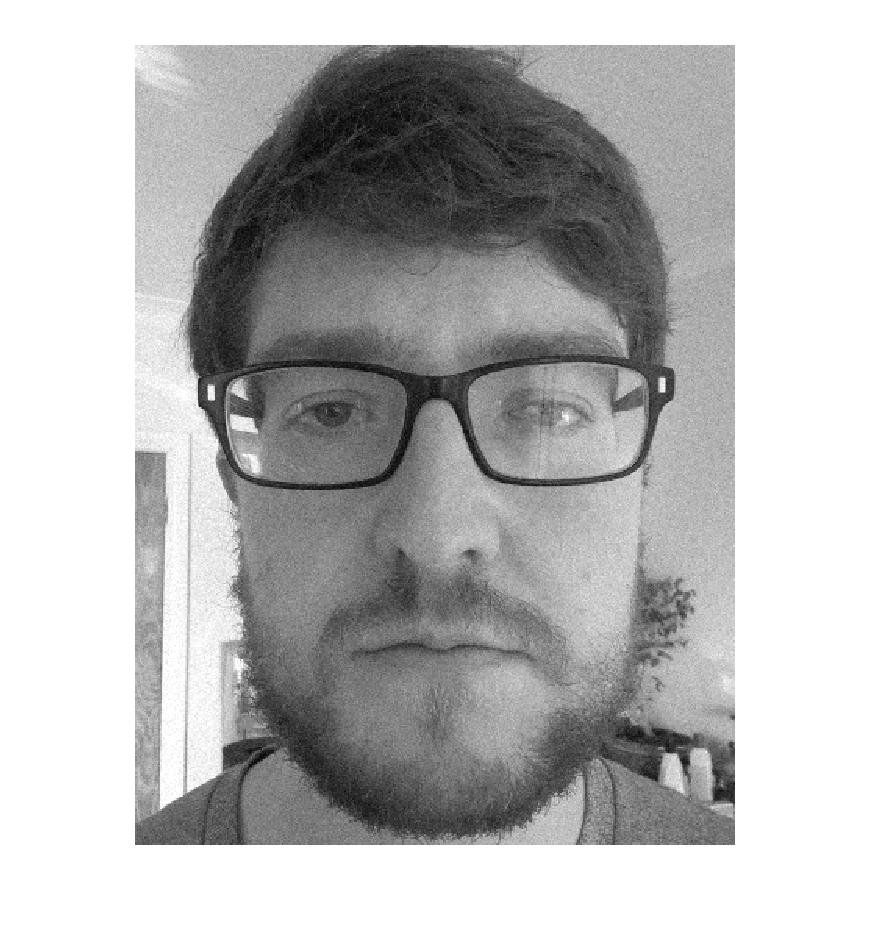
\includegraphics[height=5cm]{Results/Q1/d/qdVar0001.jpg}}%
		\subcaptionbox{Global Threshold}
		[.3\linewidth]{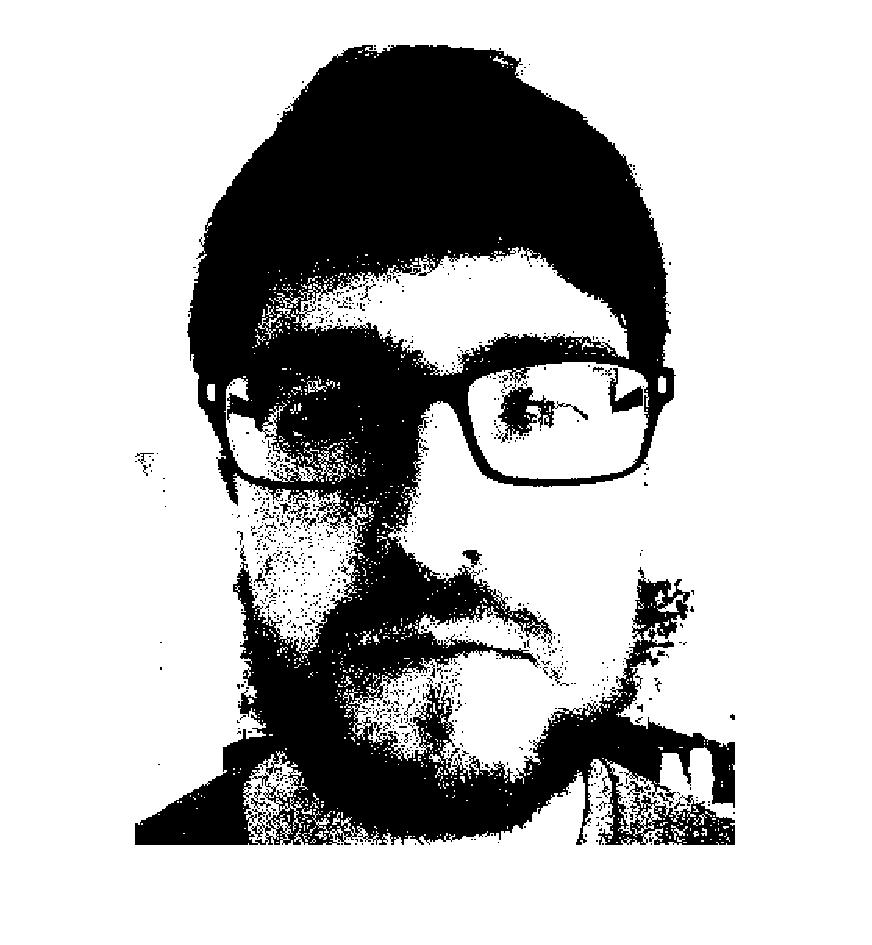
\includegraphics[height=5cm]{Results/Q1/d/qdThresh0001.jpg}}%
		\subcaptionbox{5x5 Threshold}
		[.3\linewidth]{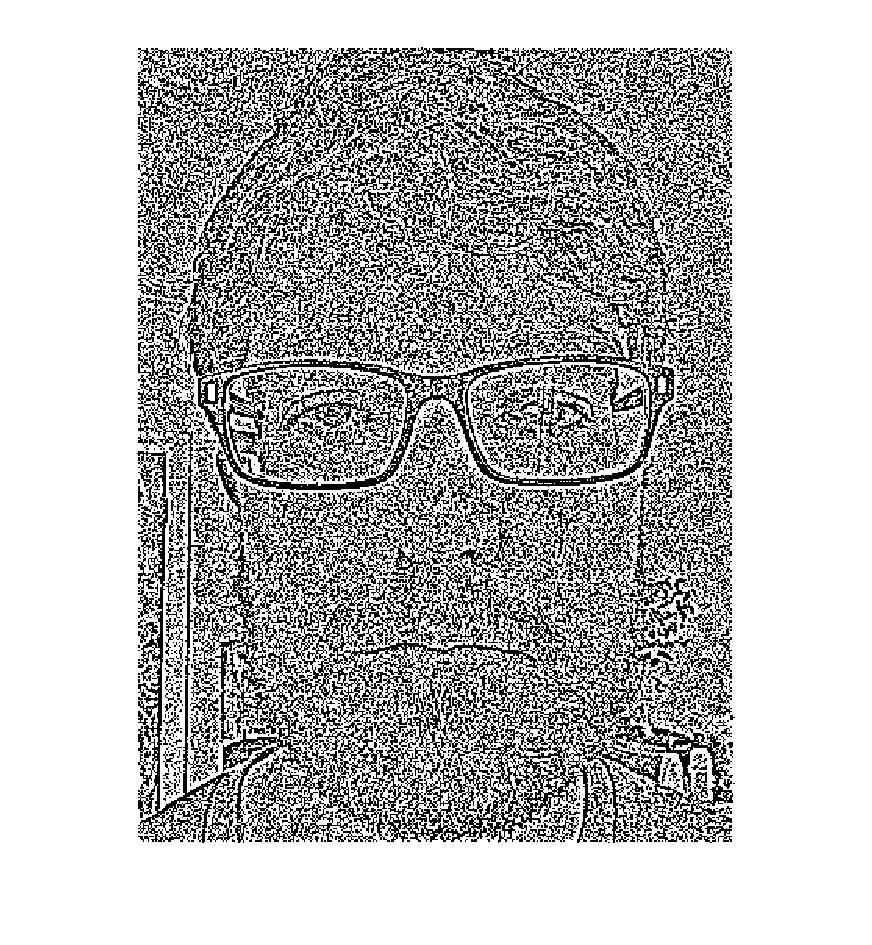
\includegraphics[height=5cm]{Results/Q1/d/qd5x50001.jpg}}%
		\caption{Thresholded Images after Gaussian Noise (0.001 Variance)}
		\label{fig:}
	\end{figure}
	\begin{figure}[H]
		\centering
		\subcaptionbox{Noisy Image}
		[.3\linewidth]{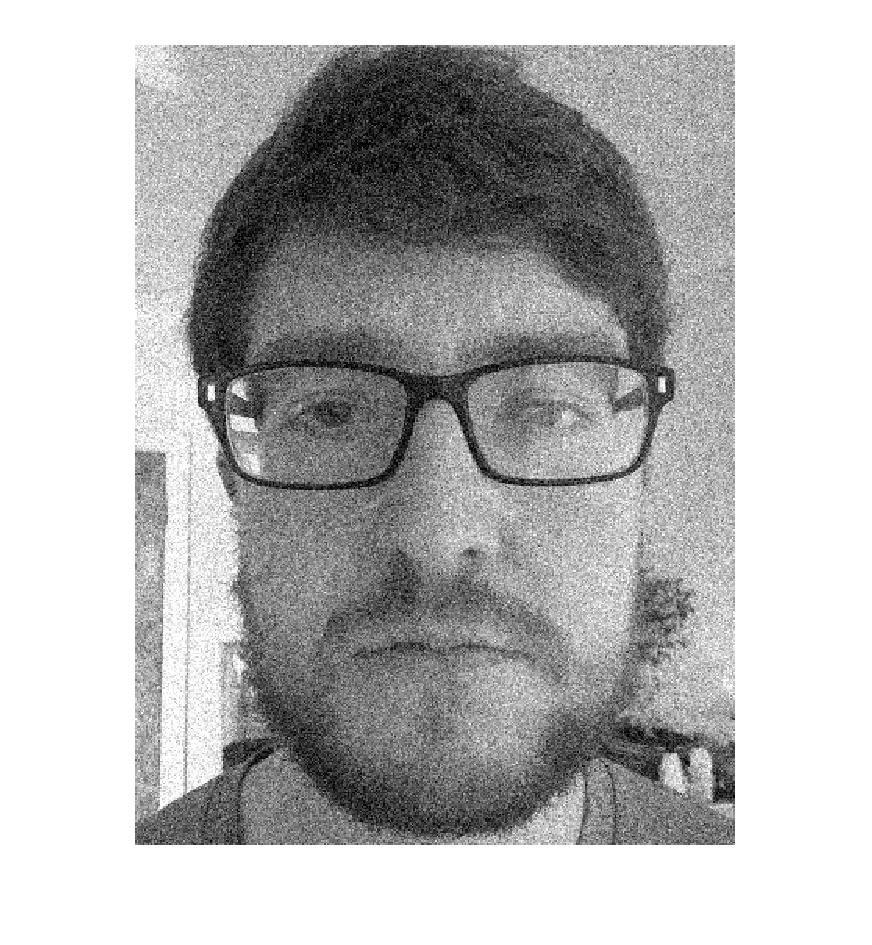
\includegraphics[height=5cm]{Results/Q1/d/qdVar001.jpg}}%
		\subcaptionbox{Global Threshold}
		[.3\linewidth]{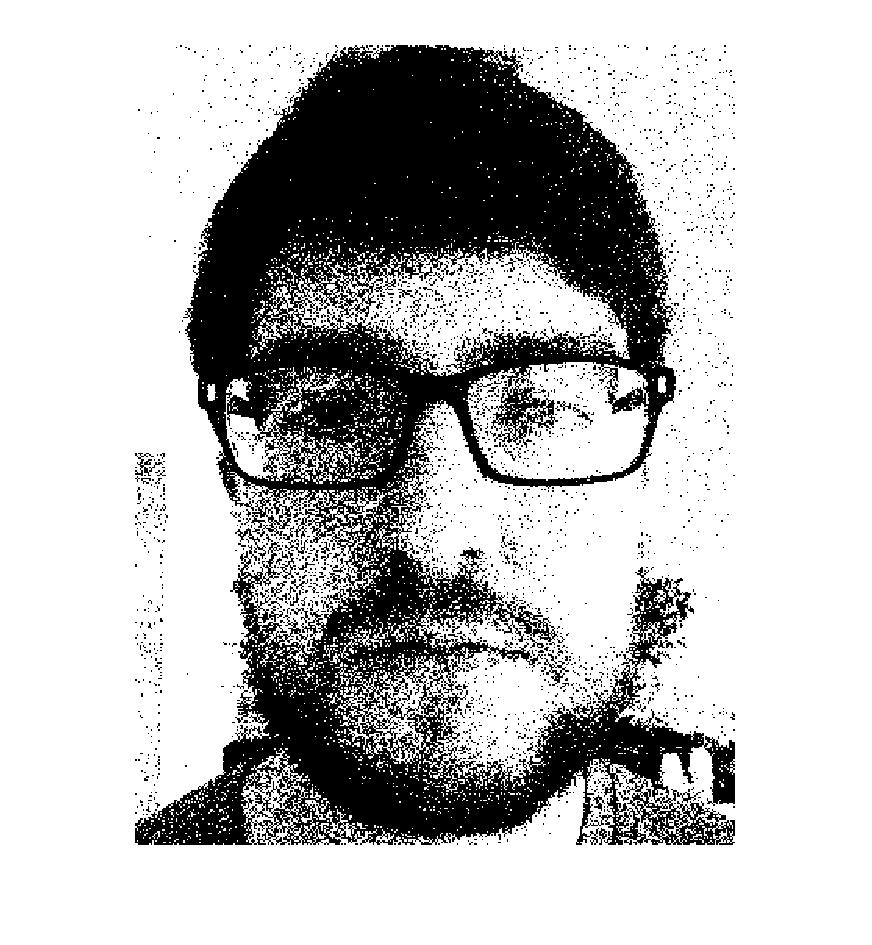
\includegraphics[height=5cm]{Results/Q1/d/qdThresh001.jpg}}%
		\subcaptionbox{5x5 Threshold}
		[.3\linewidth]{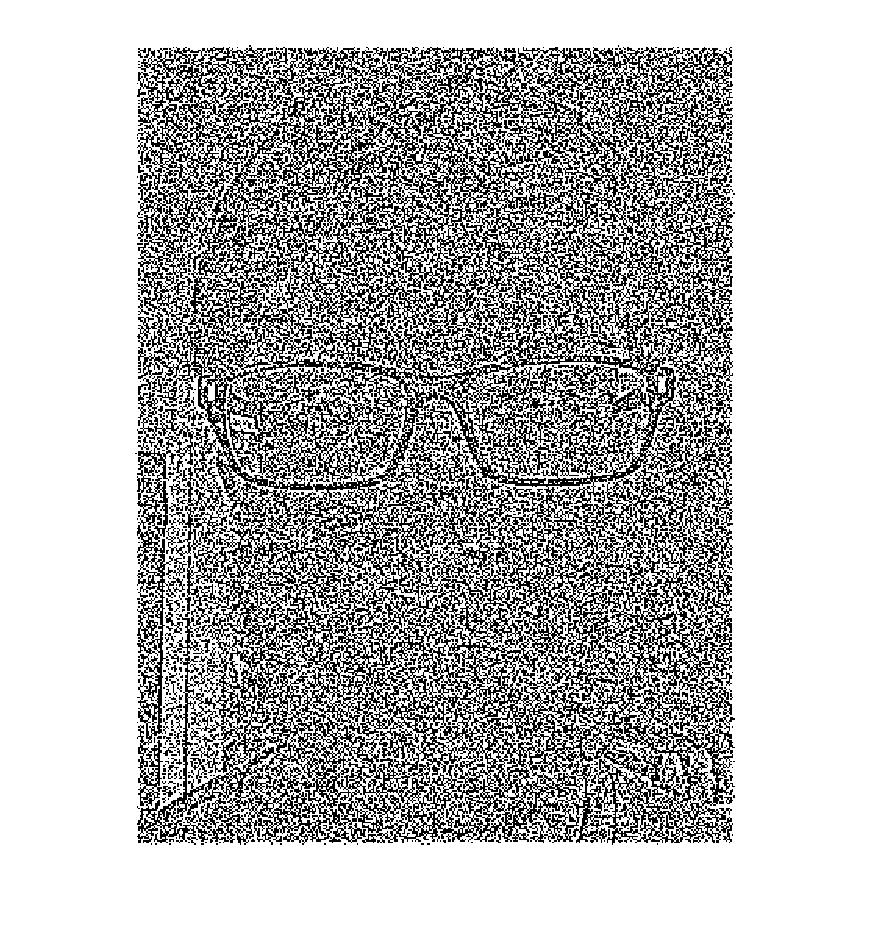
\includegraphics[height=5cm]{Results/Q1/d/qd5x5001.jpg}}%
		\caption{Thresholded Images after Gaussian Noise (0.01 Variance)}
		\label{fig:}
	\end{figure}
	\begin{figure}[H]
		\centering
		\subcaptionbox{Noisy Image}
		[.3\linewidth]{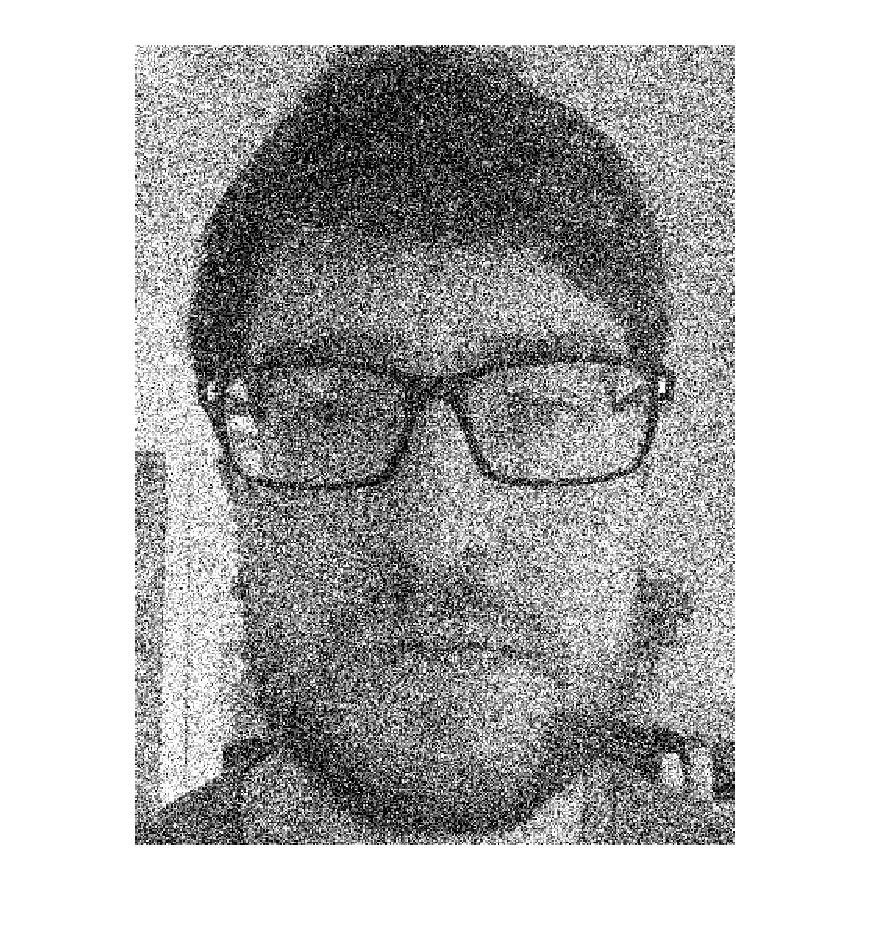
\includegraphics[height=5cm]{Results/Q1/d/qdVar01.jpg}}%
		\subcaptionbox{Global Threshold}
		[.3\linewidth]{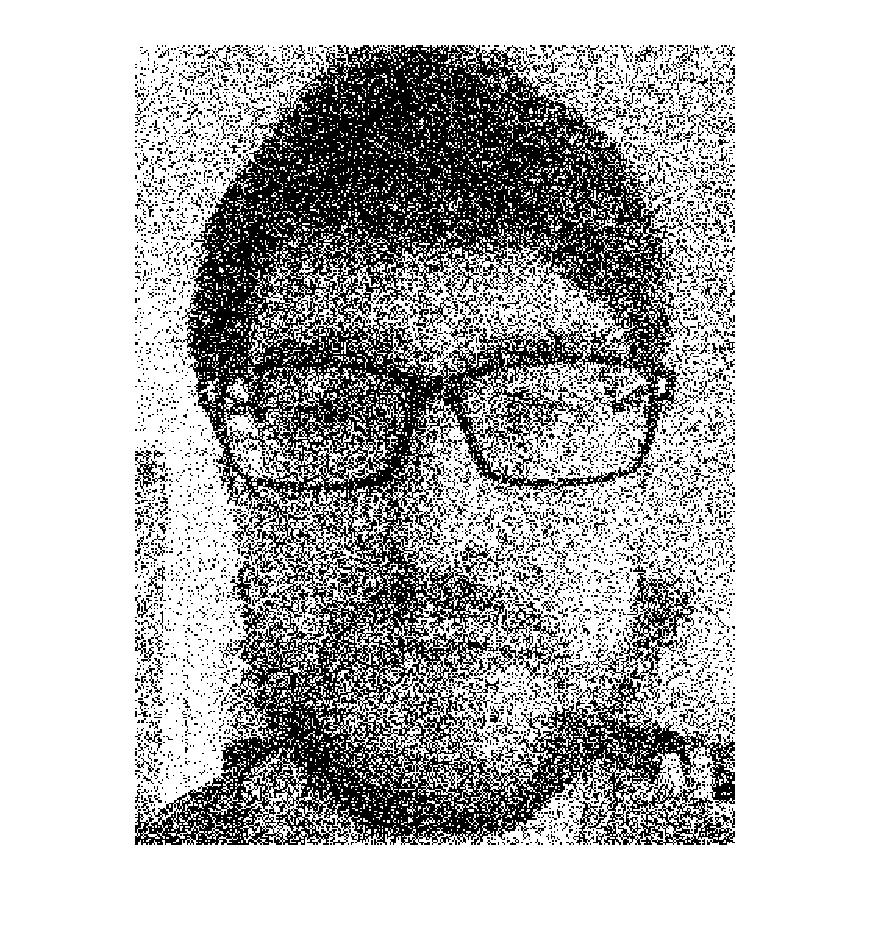
\includegraphics[height=5cm]{Results/Q1/d/qdThresh01.jpg}}%
		\subcaptionbox{5x5 Threshold}
		[.3\linewidth]{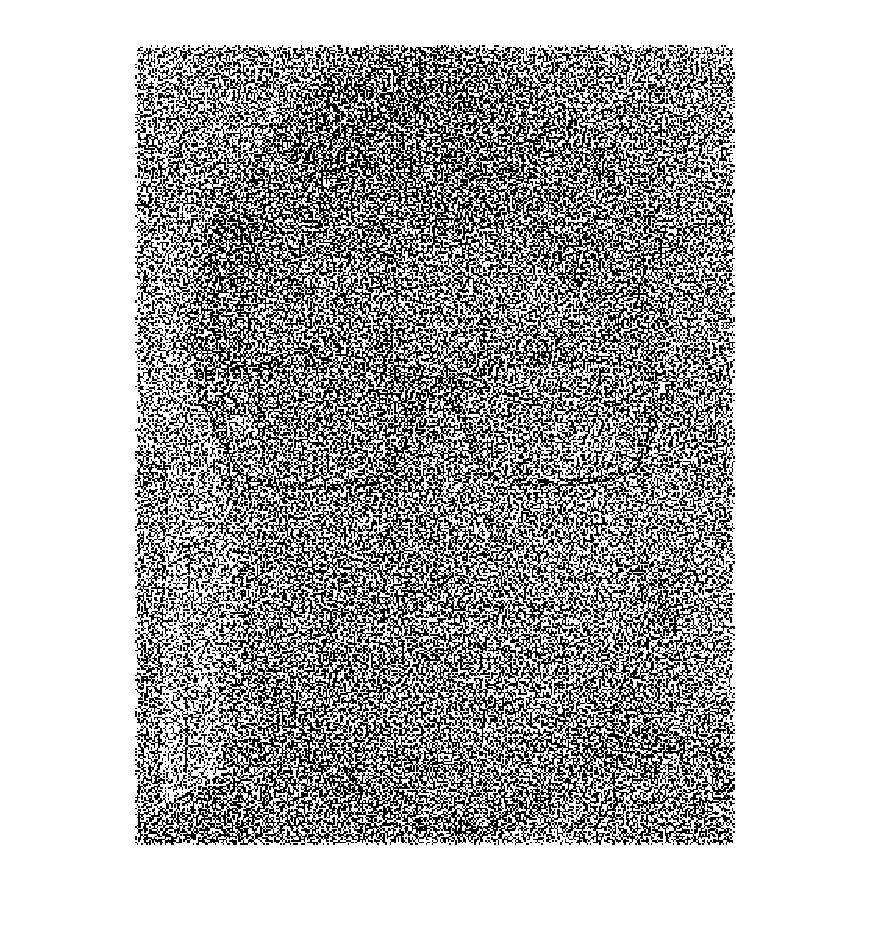
\includegraphics[height=5cm]{Results/Q1/d/qd5x501.jpg}}%
		\caption{Thresholded Images after Gaussian Noise (0.1 Variance)}
		\label{fig:}
	\end{figure}
	\begin{figure}[H]
		\centering
		\subcaptionbox{Noisy Image}
		[.3\linewidth]{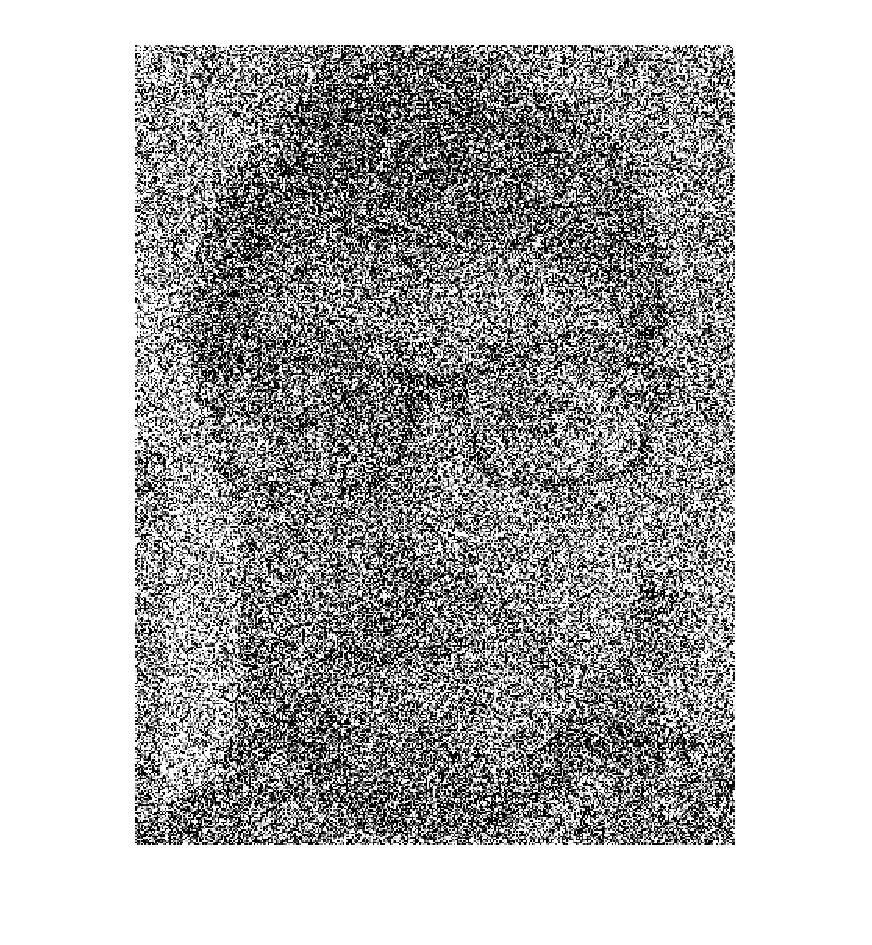
\includegraphics[height=5cm]{Results/Q1/d/qdVar1.jpg}}%
		\subcaptionbox{Global Threshold}
		[.3\linewidth]{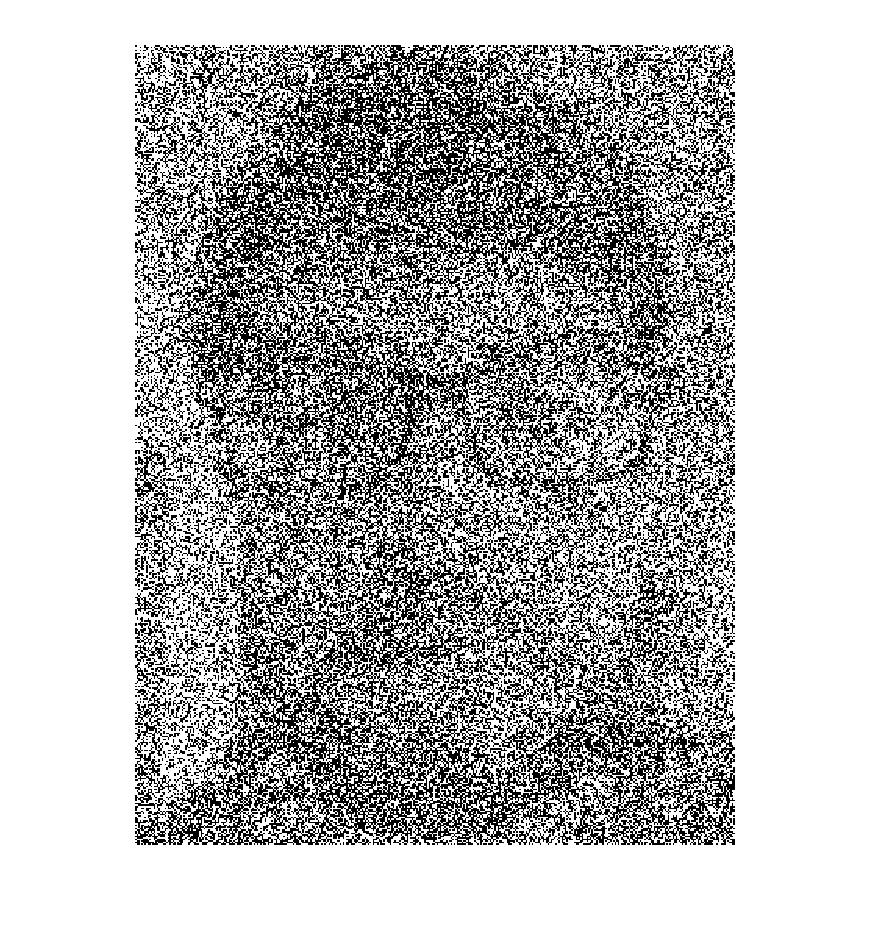
\includegraphics[height=5cm]{Results/Q1/d/qdThresh1.jpg}}%
		\subcaptionbox{5x5 Threshold}
		[.3\linewidth]{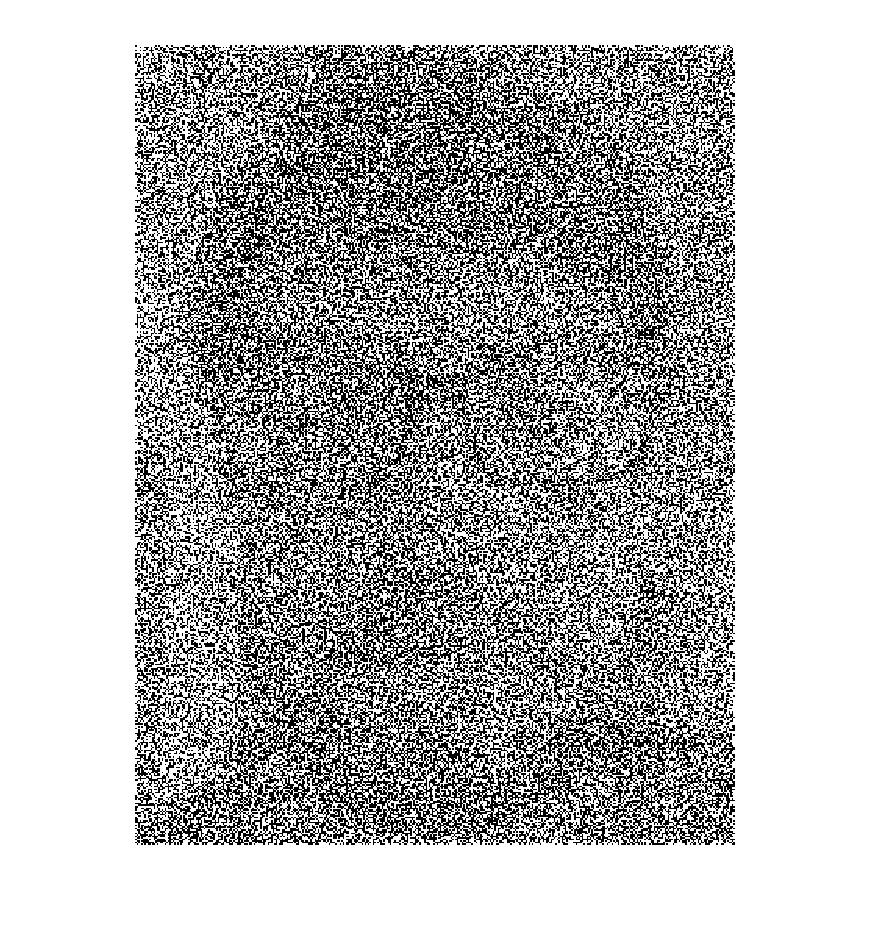
\includegraphics[height=5cm]{Results/Q1/d/qd5x51.jpg}}%
		\caption{Thresholded Images after Gaussian Noise (1 Variance)}
		\label{fig:}
	\end{figure}
	\par It can be seen that until a variance of approximately 0.01, the
	global threshold output provides good separation of the background and
	foreground, with good segmentation of the facial features.
	\par At a variance value of 0.1, there is less separation of the
	foreground and background, however, the facial features are still
	visible.
	\par The final tested noise variance is a value of 1, at which point the
	global and adaptive thresholds provide similar levels of separation.
	\subsection{Conclusion}
	Inspection of the workspace following this section shows the data types
	and dimensions of the structures used.
	\par The workspace of part a shows the reduction of the dimensions from
	the input image to the greyscale image. The removal of the three
	channels representing RGB colour allows for much faster computations,
	due to a reduction in data to be processed.
	\begin{figure}[H]
		\centering
		\includegraphics[height=5cm]{Results/Q1/a/Workspace.jpg}%
		\caption{Part a Workspace}
		\label{fig:}
	\end{figure}
	\par The workspace of part b shows the dimensions of the images,
	following the threshold function. The images are of the same dimension
	as the input image, however their values are stored as type ``double''
	rather than integer.
	\par The ``data driven'' threshold value can be seen as being calculated
	as 199. This threshold value, when applied to the image, was determined
	to be suboptimal. As such, alternative values for the threshold value
	were tested, with the optimal choice being 125.
	\par Choosing the optimal threshold value for a global threshold
	function is difficult for a number of reasons, namely uneven lighting
	conditions, and, in the case of the input images, irregular surfaces
	such as glasses and facial hair. These features cause the shadowing on
	the left side of the image, the streak covering the left eye (a shine on
	the glasses), and the blurring surrounding the lips.
	\begin{figure}[H]
		\centering
		\includegraphics[height=5cm]{Results/Q1/b/Workspace.jpg}%
		\caption{Part b Workspace}
		\label{fig:}
	\end{figure}
	\par The final workspace of the 5x5 Adaptive Threshold show the
	dimensions of the output image, which are the same as the input
	greyscale image, and of type ``double''.
	\par The 5x5 adaptive threshold, thresholding each pixel based on the
	average of the surrounding 5x5 region, provides adequate segmentation of
	the background and foreground. It also deals with issues such as uneven
	lighting conditions, glasses and reflections, and facial hair, with a
	better accuracy than the global threshold. The resulting image has
	better segmentation of the facial features, and better separation of the
	foreground and background.
	\begin{figure}[H]
		\centering
		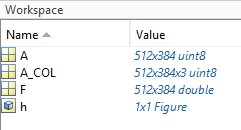
\includegraphics[height=5cm]{Results/Q1/c/Workspace.jpg}%
		\caption{Part c Workspace}
		\label{fig:}
	\end{figure}
	\par The final workspace of part d shows the resulting dimensions of
	both the adaptive and global threshold functions, as applied to the
	noisy input greyscale image.
	\par From the results section above, it is clear that the global
	threshold technique is less sensitive to noise. As there is no weight
	placed on the pixel intensity values within the image, there is less
	variance to the thresholding with the amount of noise found in the image.
	\par As the adaptive thresholding relies strongly on the intensity
	values in the pixels surrounding the pixel in question, noise can have a
	greater effect on the thresholding.
	\begin{figure}[H]
		\centering
		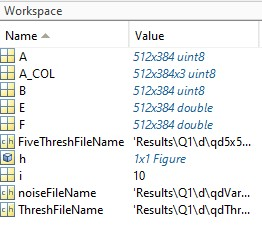
\includegraphics[height=5cm]{Results/Q1/d/Workspace.jpg}%
		\caption{Part d Workspace}
		\label{fig:}
	\end{figure}
	The code utilised in the completion of this section can be found in the
	Appendices.
	\section{Part 2: Segmentation}
	\subsection{Introduction}
	Segmentation is the practice of extracting features from an image. In
	this section, the main alphanumeric registration characters of a licence
	plate must be extracted from the overall image. The extracted characters
	must not include either the country code, county name, or dashes between
	sections of the registration.
	\par Automated and data driven segmentation can be achieved by combining
	arithmetic functions and blob functions. As the size ratio of each letter in
	the registration does not change with scale, this ratio can be utilised
	to remove only blobs under a size specified by the largest letter
	(blob).
	\subsection{Techniques}
	In completing this section of the assignment, the following techniques
	are utilised:
	\subsubsection{Part a}
	\underline{\textbf{Low Pass Filter}}
	\par The VSG ``LowPass'' filter function applies a 3x3 low pass filter
	to the image.
	\par\underline{\textbf{Mid-Threshold}}
	\par Much like the aforementioned ``Threshold'' function, the
	``MidThresh'' function applies a single threshold value to the image.
	The threshold value chosen is 125, the middle of the 0-255 range of the
	integer input values.
	\par\underline{\textbf{Inversion (NOT)}}
	\par Inversion is achieved using the VSG ``NOT'' function, which
	performs a boolean Not operation on each pixel of the image. On a binary
	image, this changes all white pixels to black, and all black pixels to
	white.
	\par\underline{\textbf{Biggest Blob}}
	\par The ``BiggestBlob'' function of the VSG toolbox outputs an image
	containing only the biggest single white blob from the binary input
	image.
	\par\underline{\textbf{Subtract}}
	\par The VSG ``Subtract'' function performs matrix subtraction between the
	specified images. Each pixel of the input image has its value
	subtracted from the corresponding pixel in the other image. As in this
	section, if one	image is binary, and the other RGB colour, the binary
	image is subtracted from the red channel of the RGB image.
	\par\underline{\textbf{White Pixel Counter}}
	\par The VSG ``WPCounter'' function counts the number of white pixels
	within the input image, outputting its value as an integer.
	\par\underline{\textbf{Mask}}
	\par The VSG ``MaskImg'' function applies a border mask of the input
	thickness to the image. The masked pixels which fall within the
	thickness have their values set to 0 (black).
	\par\underline{\textbf{Exclusive Or (XOR)}}
	\par The Exclusive Or function is completed using the VSG ``XOR''
	function. A bitwise XOR operation applied to binary images returns a
	white pixel only if the pixel is white in exactly one of the two input
	images.
	\par\underline{\textbf{Count Blobs}}
	\par The ``CountBlobs'' function of the VSG toolbox counts the number of
	white blobs in the input image, outputting its value as an integer.
	\par\underline{\textbf{Canny}}
	\par The VSG ``Canny'' edge detection function returns the image with
	any edges highlighted.
	\par\underline{\textbf{Add}}
	\par The VSG ``Add'' function performs matrix addition between the
	specified images. Each pixel of the input image has its value added to
	the corresponding pixel in the other image. As in this section, if one
	image is binary, and the other RGB colour, the binary image is added to
	the red channel of the RGB image.
	\subsection{Pseudocode}
	\subsubsection{Part a}
	\begin{enumerate}
		\item Load the image into Matlab using the ``imread()''
			function
		\item Use the ``rgb2gray()'' function to convert the image to
			greyscale.
		\item Display the greyscale image using the ``imshow()''
			function.
		\item Apply a low pass filter, using the VSG ``LowPass'' function,
			to remove noise from the image.
		\item Apply a threshold to the image using the VSG
			``MidThreshold'' function.
		\item Invert the image using the VSG ``NOT'' function.
		\item Extract the biggest blob (Country code and outer border),
			using the ``BiggestBlob'' VSG function.
		\item Subtract the extracted biggest blob image from the original
			image using the VSG ``Subtract'' function.
		\item Extract the biggest blob, using the ``BiggestBlob''
			function, (the largest alphanumeric character in the
			registration) .
		\item Using the VSG package ``WPCounter'' function, count the
			number of pixels in the biggest blob.
		\item Apply a single pixel mask to the image in order to remove
			the white pixel border.
		\item Compare the next biggest blob with the biggest blob, if
			the size is within the given ratio, ``XOR'' this with the
			image containing the previous biggest blob. Subtract
			this blob from the original image to avoid unintended
			looping. Repeat until the blob checked does not match
			the given ratio.
		\item Count the number of blobs in the resulting image using the
			VSG ``CountBlobs'' function.
		\item Use the VSG 'Canny' function to output an edge detector
			representation of the extracted characters.
		\item Overlay the resulting image on the original input image
			using the VSG 'Add' function.
	\end{enumerate}
	\subsubsection{Part b}
	\begin{enumerate}
		\item Apply ``imnoise()'' to the greyscale image, repeating the
			steps in part a.
		\item Increase the variance until the incorrect output value is
			acquired.
	\end{enumerate}
	\subsection{Results}
	\subsubsection{Part a}
	In part a, the alphanumeric registration characters of the licence plate
	are correctly extracted. The licence plate image is first loaded into
	Matlab, converted to greyscale, and a low pass filter is applied.
	\begin{figure}[H]
		\centering
		\subcaptionbox{Input Image}
		[.3\linewidth]{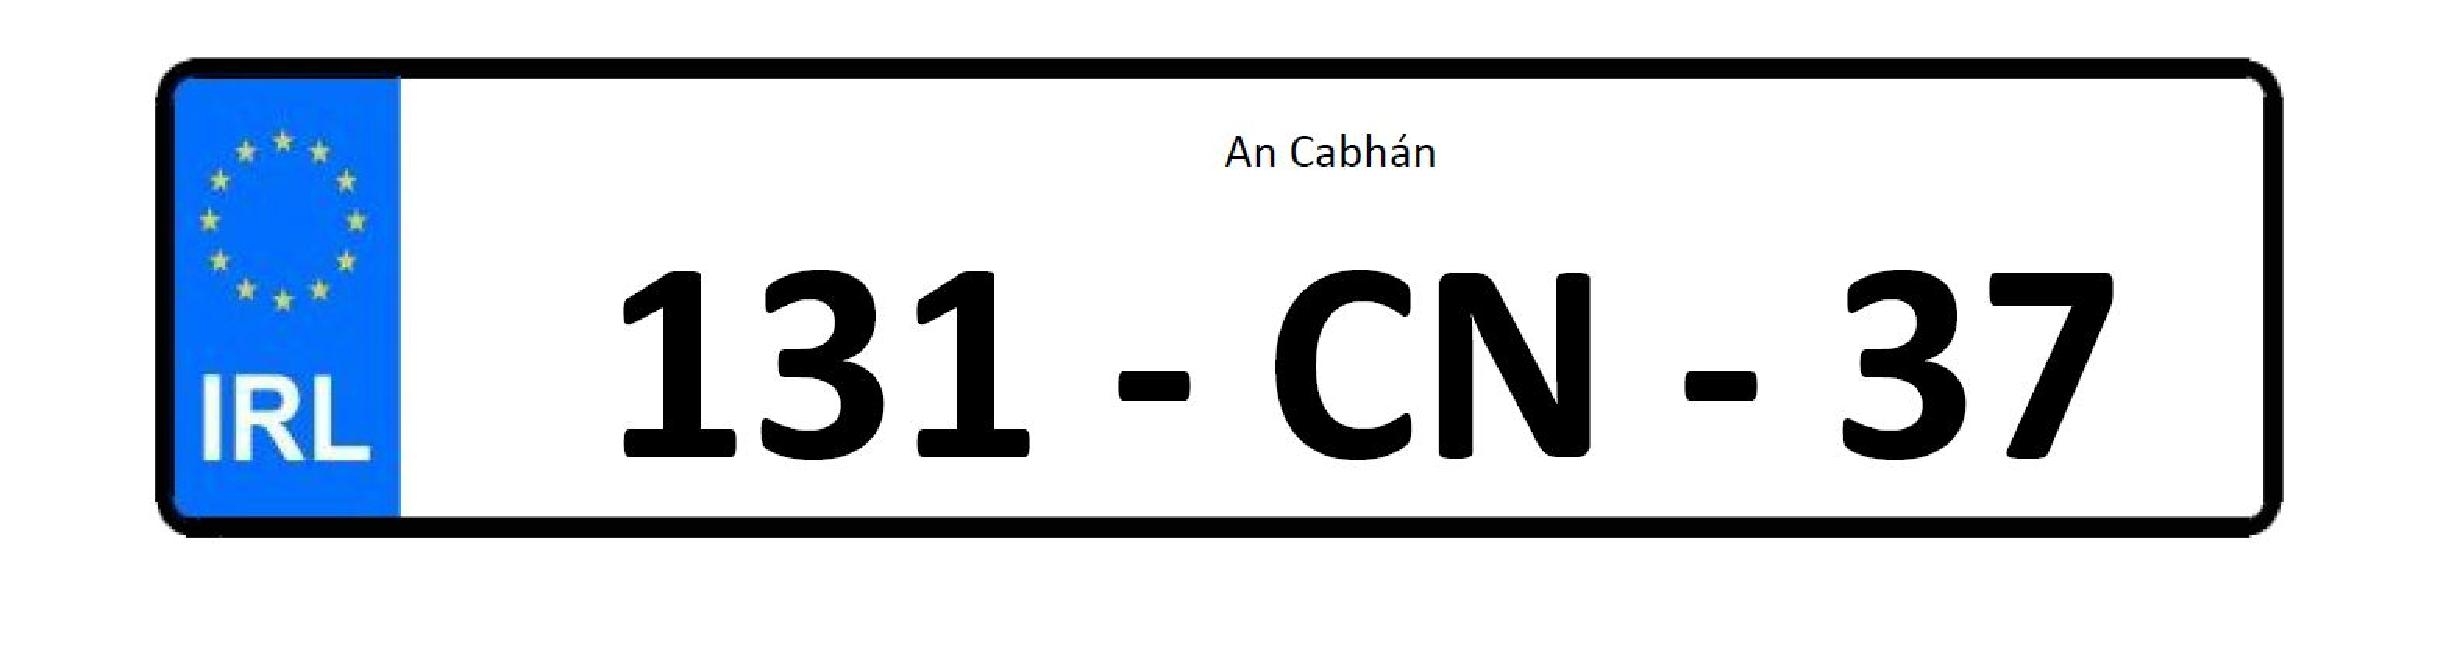
\includegraphics[height=1cm]{Results/Q2/NumPlate1/qanumber_plate_1.jpg}}%
		\subcaptionbox{Greyscale Image}
		[.3\linewidth]{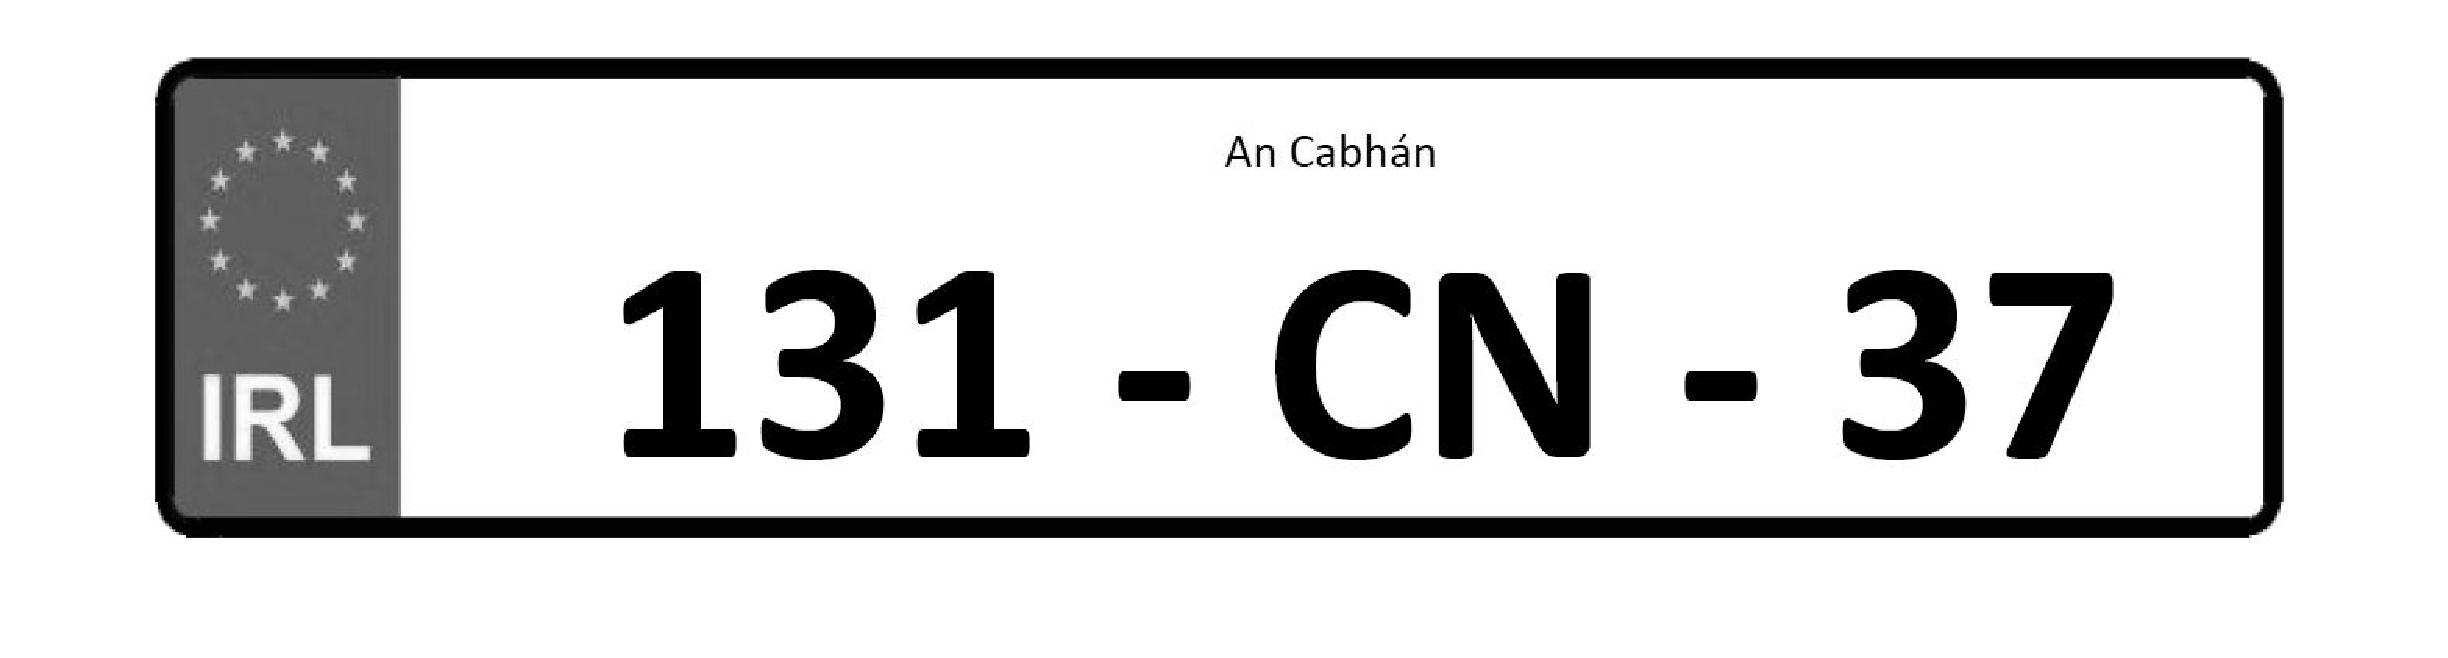
\includegraphics[height=1cm]{Results/Q2/NumPlate1/qanumber_plate_1Grey.jpg}}%
		\subcaptionbox{Low Pass Filtered}
		[.3\linewidth]{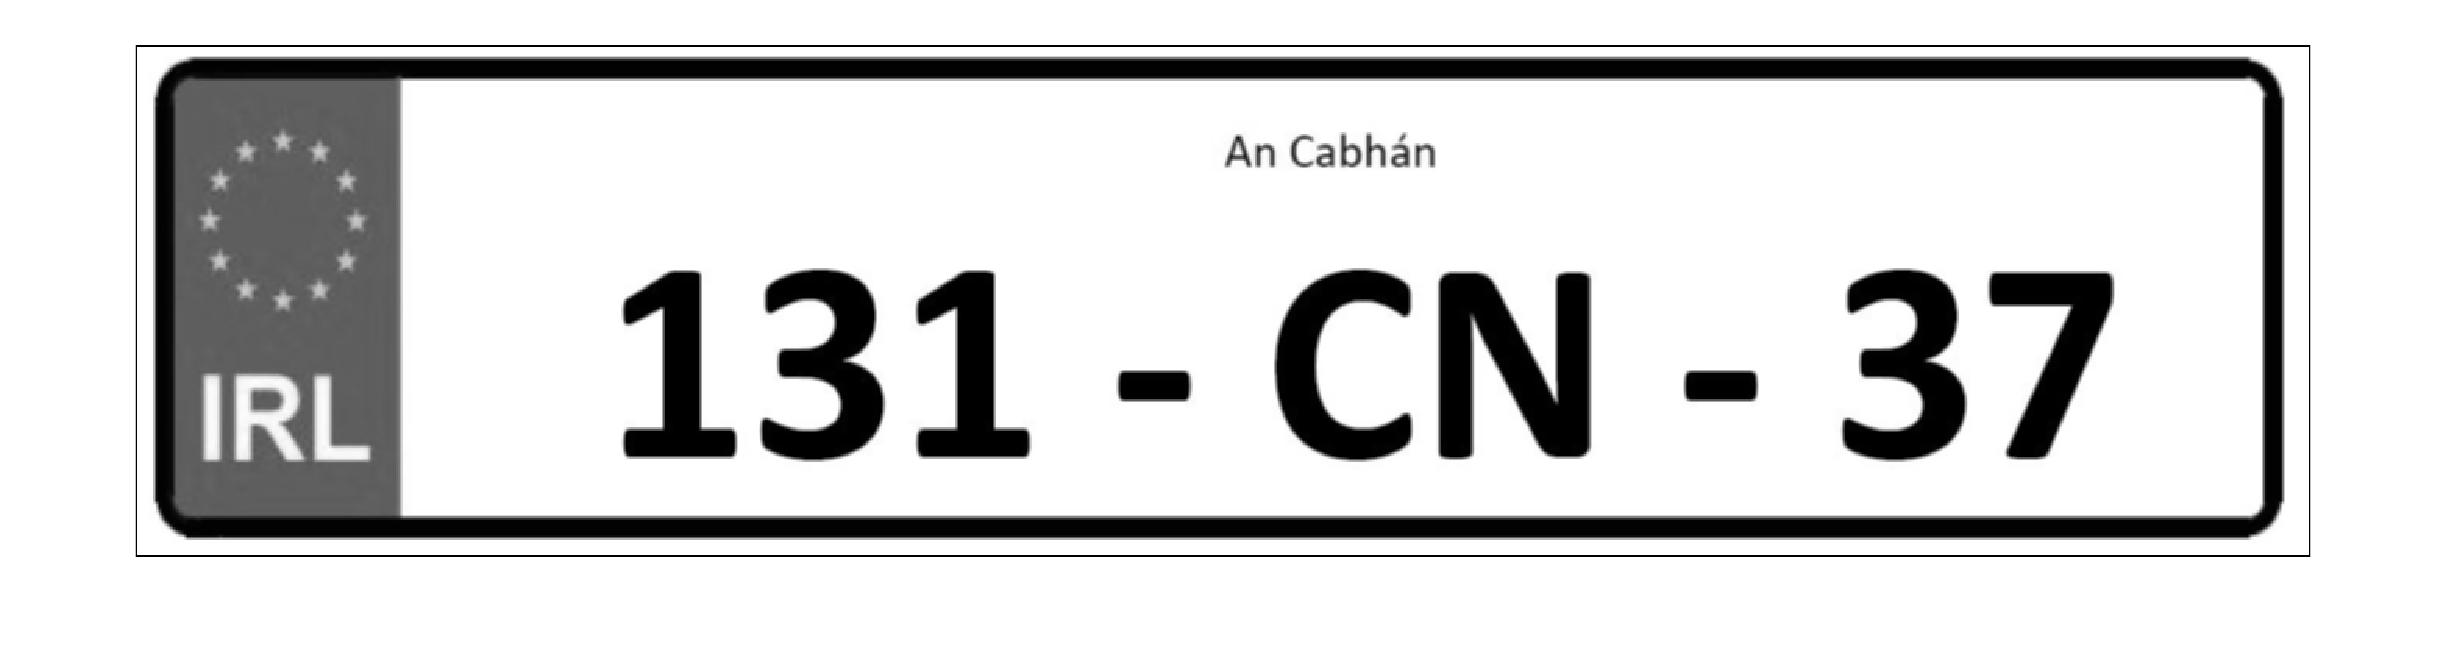
\includegraphics[height=1cm]{Results/Q2/NumPlate1/qanumber_plate_1Low.jpg}}%
		\caption{Initial Segmentation Setup}
		\label{fig:}
	\end{figure}
	\par The extraction process begins by applying a mid-value threshold to the
	image. The image is then inverted to allow for blob functions to be
	utilised. The border and country code are removed from the image by
	subtracting the biggest blob from the thresholded image.
	\begin{figure}[H]
		\centering
		\subcaptionbox{Mid Threshold}
		[.5\linewidth]{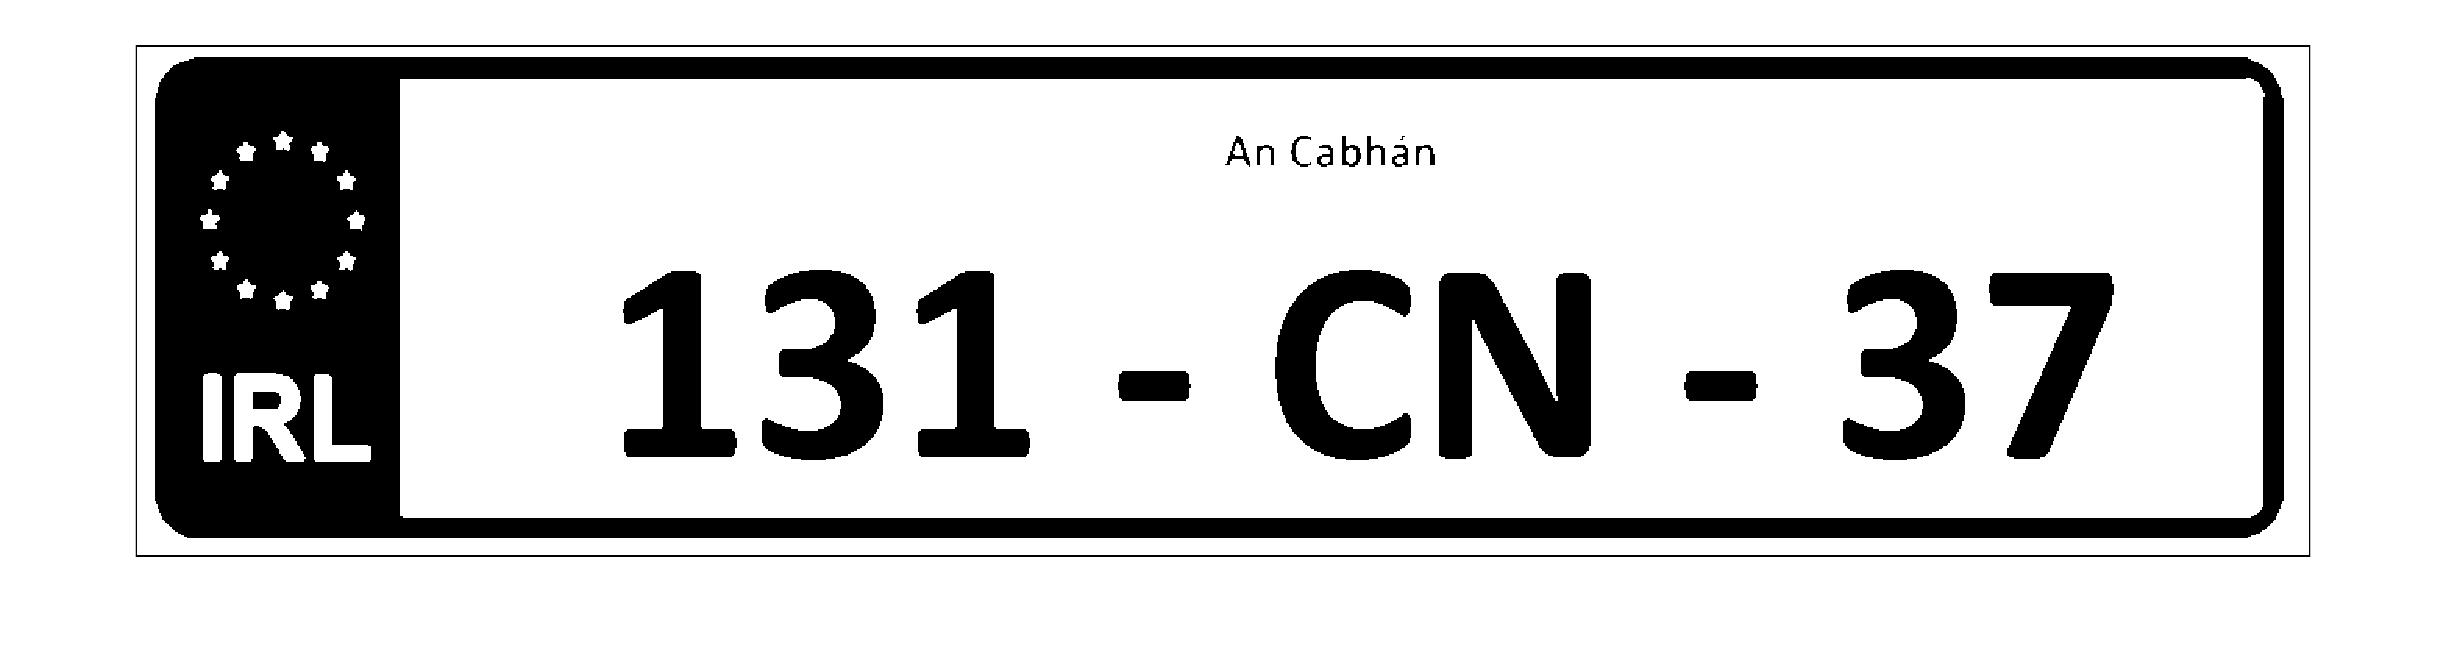
\includegraphics[height=1.5cm]{Results/Q2/NumPlate1/qanumber_plate_1Mid.jpg}}%
		\subcaptionbox{Inverted (Not)}
		[.5\linewidth]{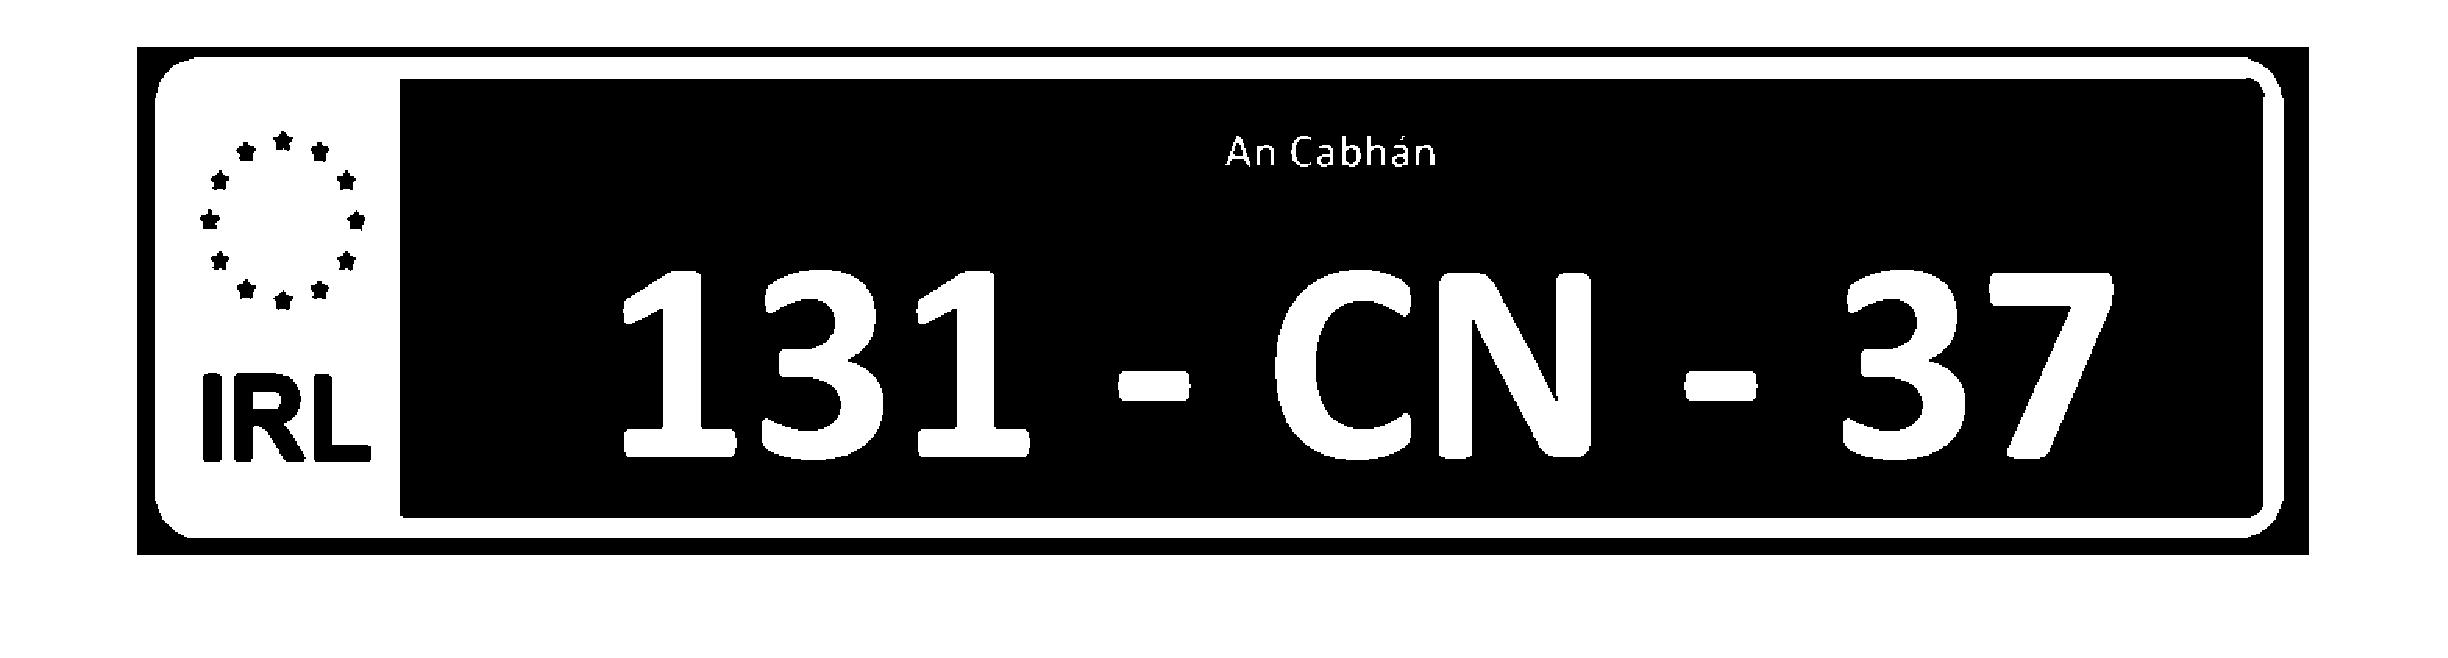
\includegraphics[height=1.5cm]{Results/Q2/NumPlate1/qanumber_plate_1Not.jpg}}%
		\caption{Preparing for Border Removal}
		\label{fig:}
	\end{figure}
	\begin{figure}[H]
		\centering
		\subcaptionbox{Biggest Blob}
		[.5\linewidth]{
\includegraphics[height=1.5cm]{Results/Q2/NumPlate1/qanumber_plate_1Border.jpg}}%
		\subcaptionbox{Biggest Blob Removed}
		[.5\linewidth]{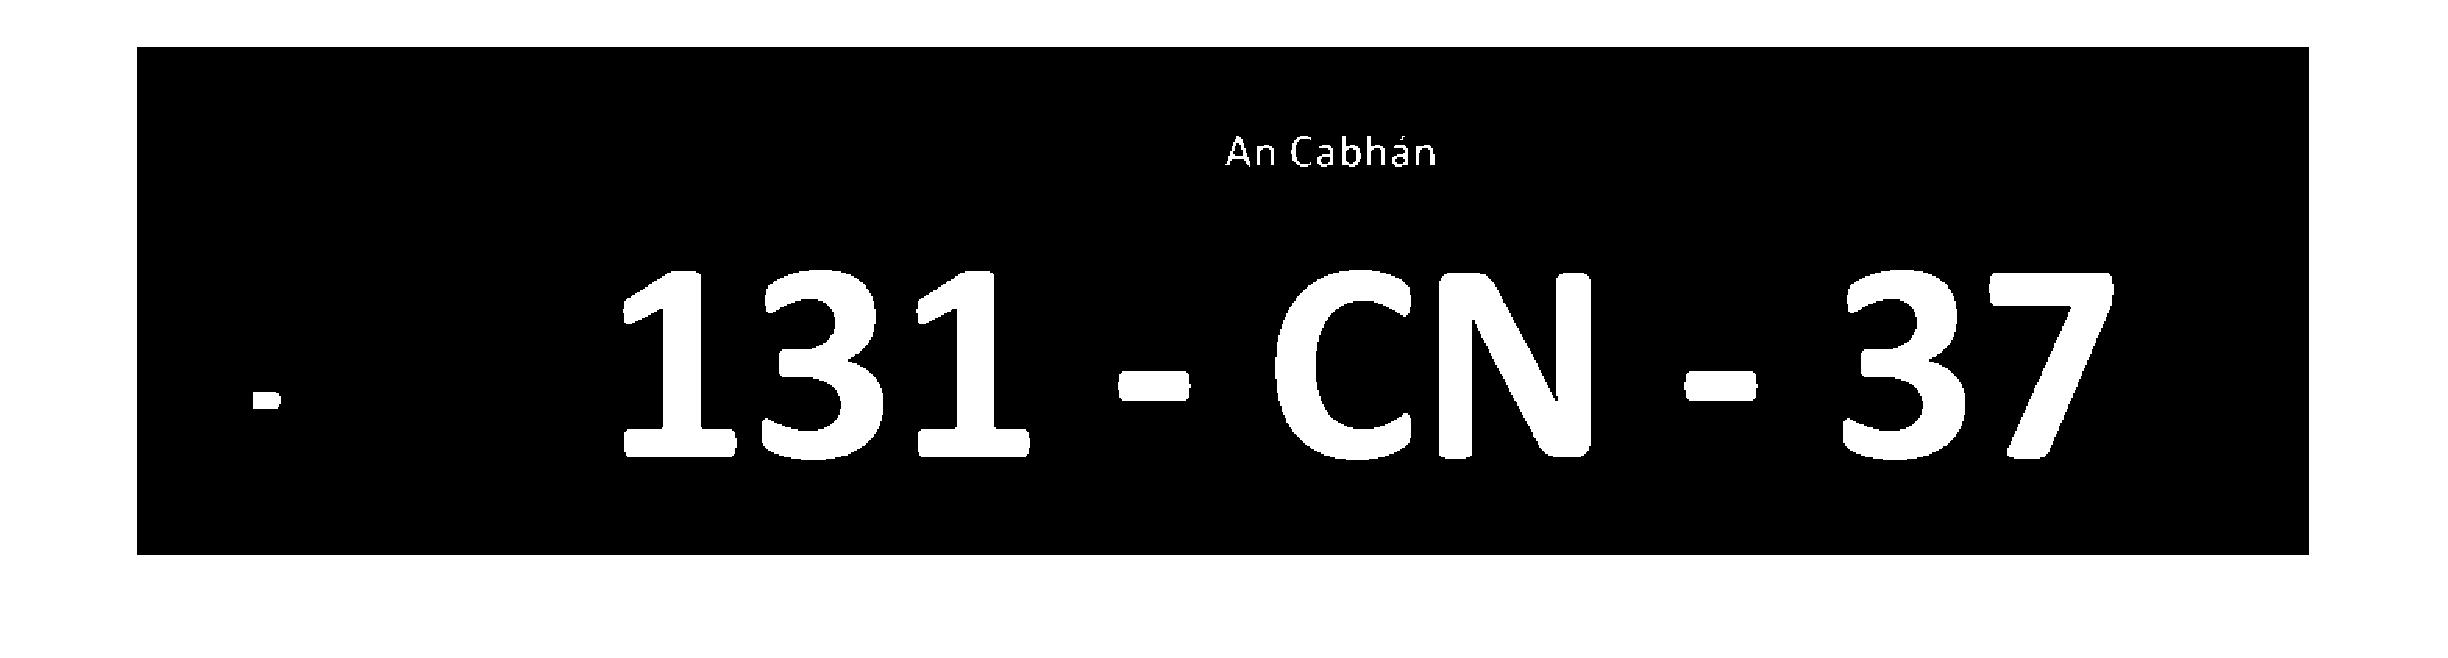
\includegraphics[height=1.5cm]{Results/Q2/NumPlate1/qanumber_plate_1NoBorder.jpg}}%
		\caption{Removed Outer Border}
		\label{fig:}
	\end{figure}
	\par Finally the main alphanumeric characters are extracted by looping
	through the blobs in the image, until the lower bound for the blob size
	is exceeded. The found blobs are then counted, and an edge detected
	version of the image is overlayed on the original image for display
	purposes.
	\begin{figure}[H]
		\centering
		\subcaptionbox{Largest Character}
		[.5\linewidth]{
\includegraphics[height=1.5cm]{Results/Q2/NumPlate1/qanumber_plate_1BigChar.jpg}}%
		\subcaptionbox{Remaining Characters}
		[.5\linewidth]{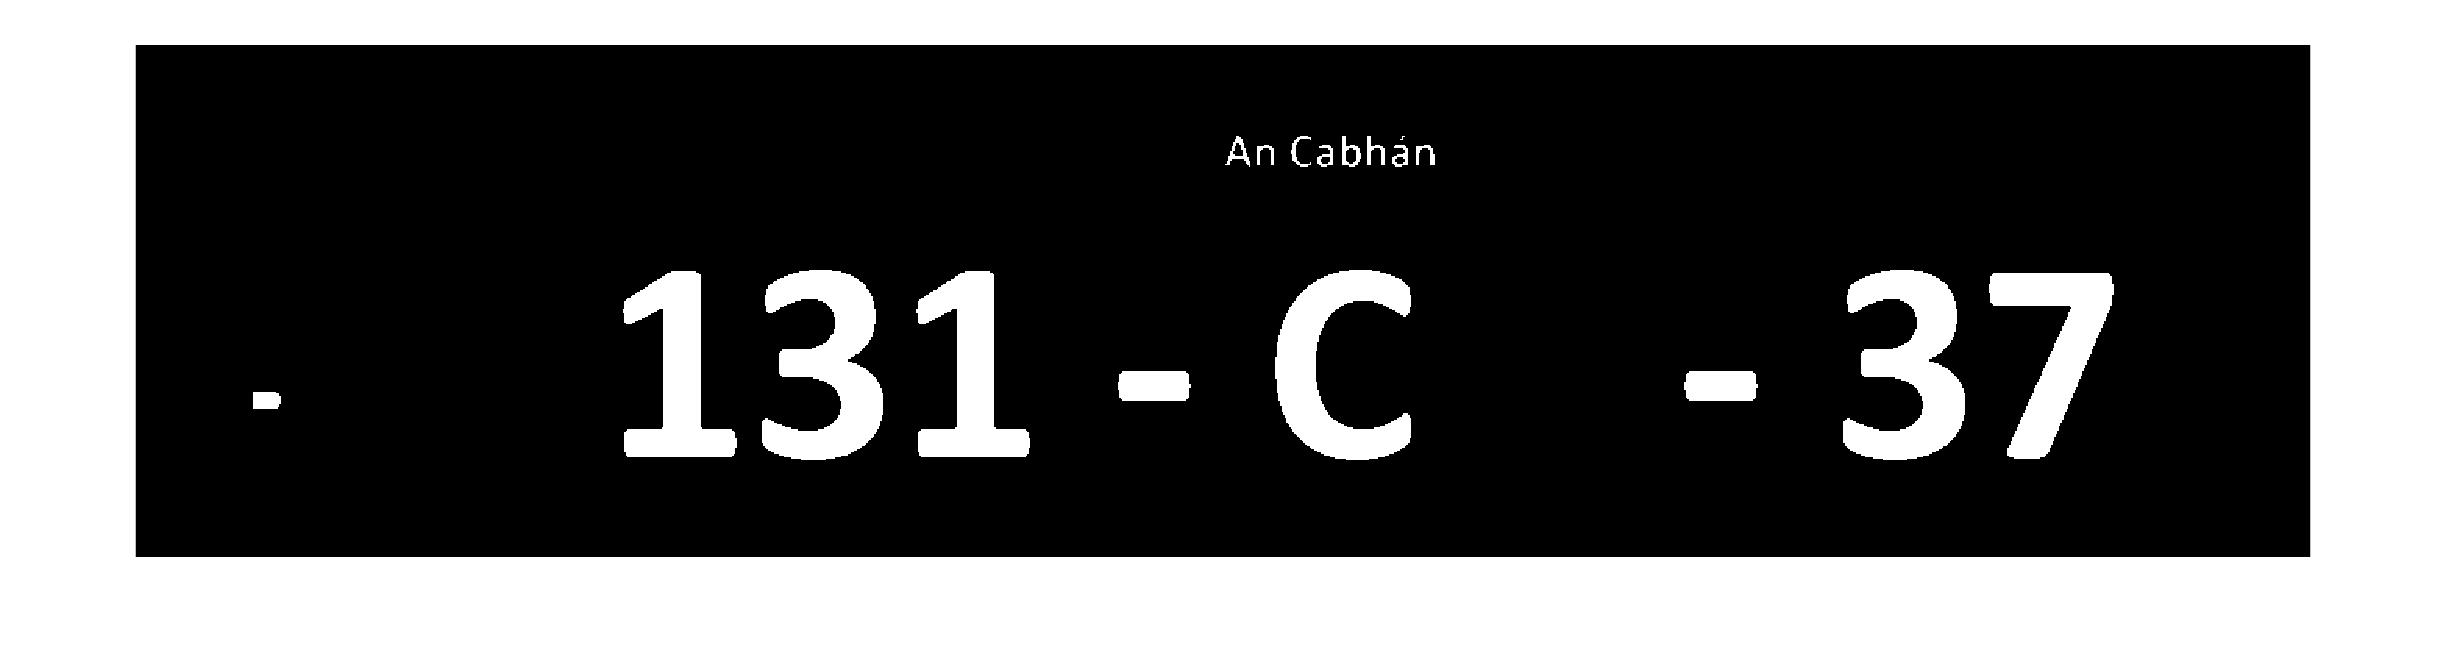
\includegraphics[height=1.5cm]{Results/Q2/NumPlate1/qanumber_plate_1Remain.jpg}}%
		\caption{Removed Largest Alphanumeric Character}
		\label{fig:}
	\end{figure}
	\begin{figure}[H]
		\centering
		\subcaptionbox{Loop 1 Result}
		[.3\linewidth]{
\includegraphics[height=1cm]{Results/Q2/NumPlate1/qanumber_plate_1Added1.jpg}}%
		\subcaptionbox{Loop 2 Result}
		[.3\linewidth]{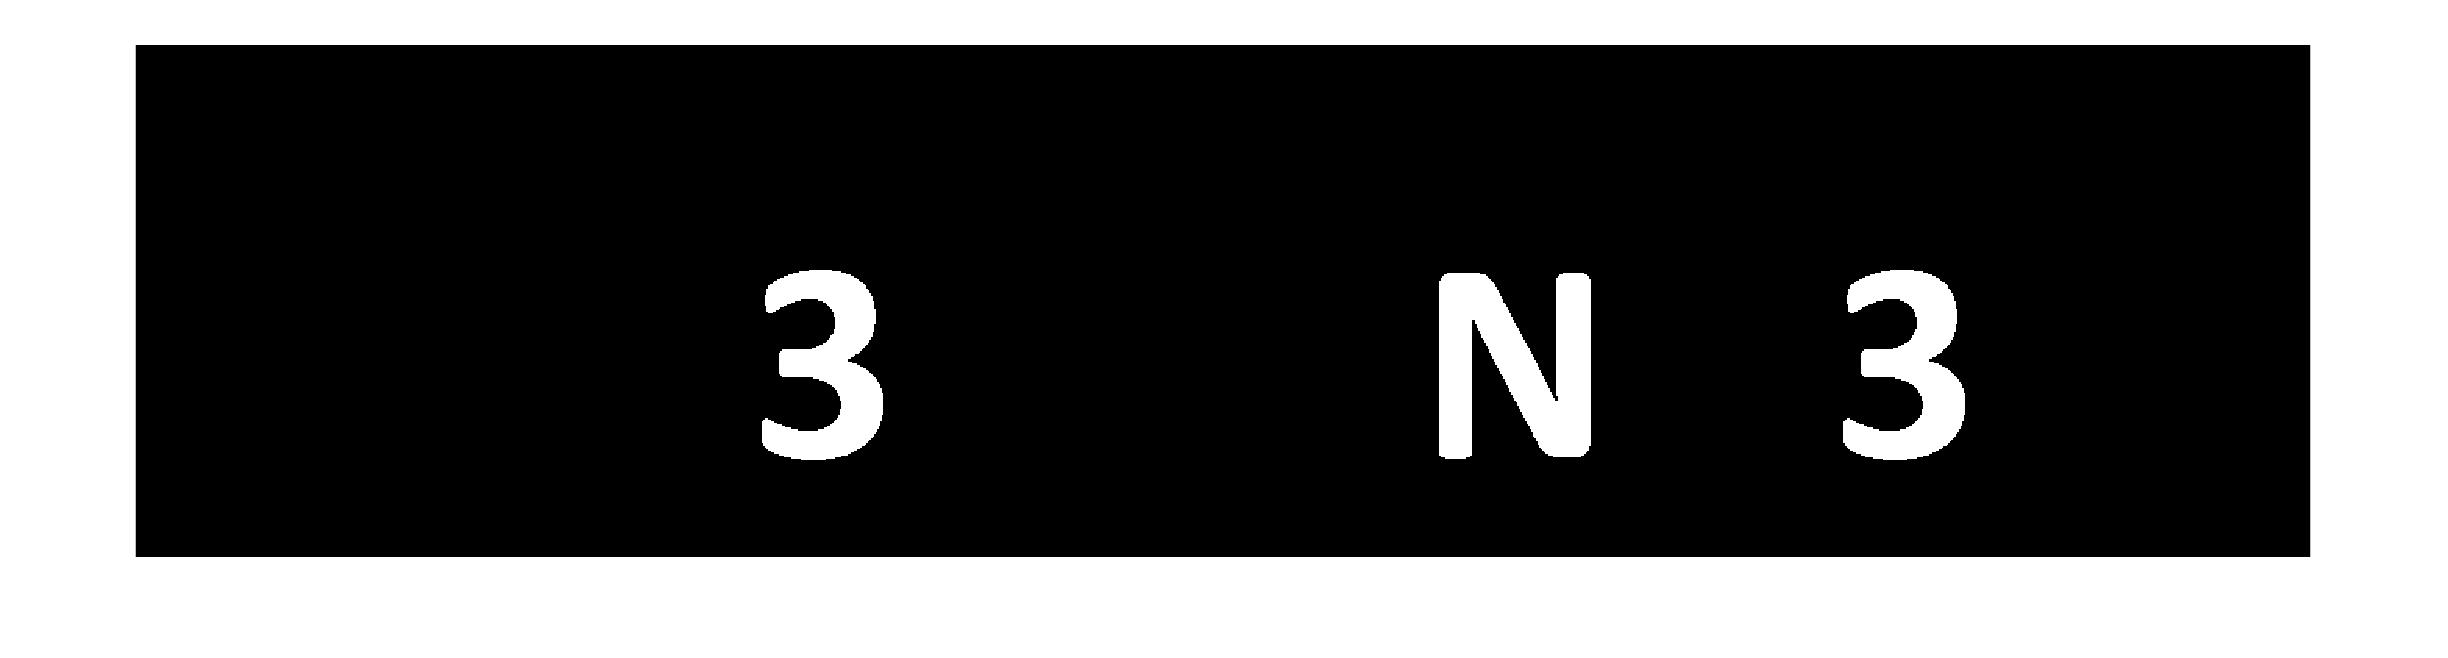
\includegraphics[height=1cm]{Results/Q2/NumPlate1/qanumber_plate_1Added2.jpg}}%
		\subcaptionbox{Loop 3 Result}
		[.3\linewidth]{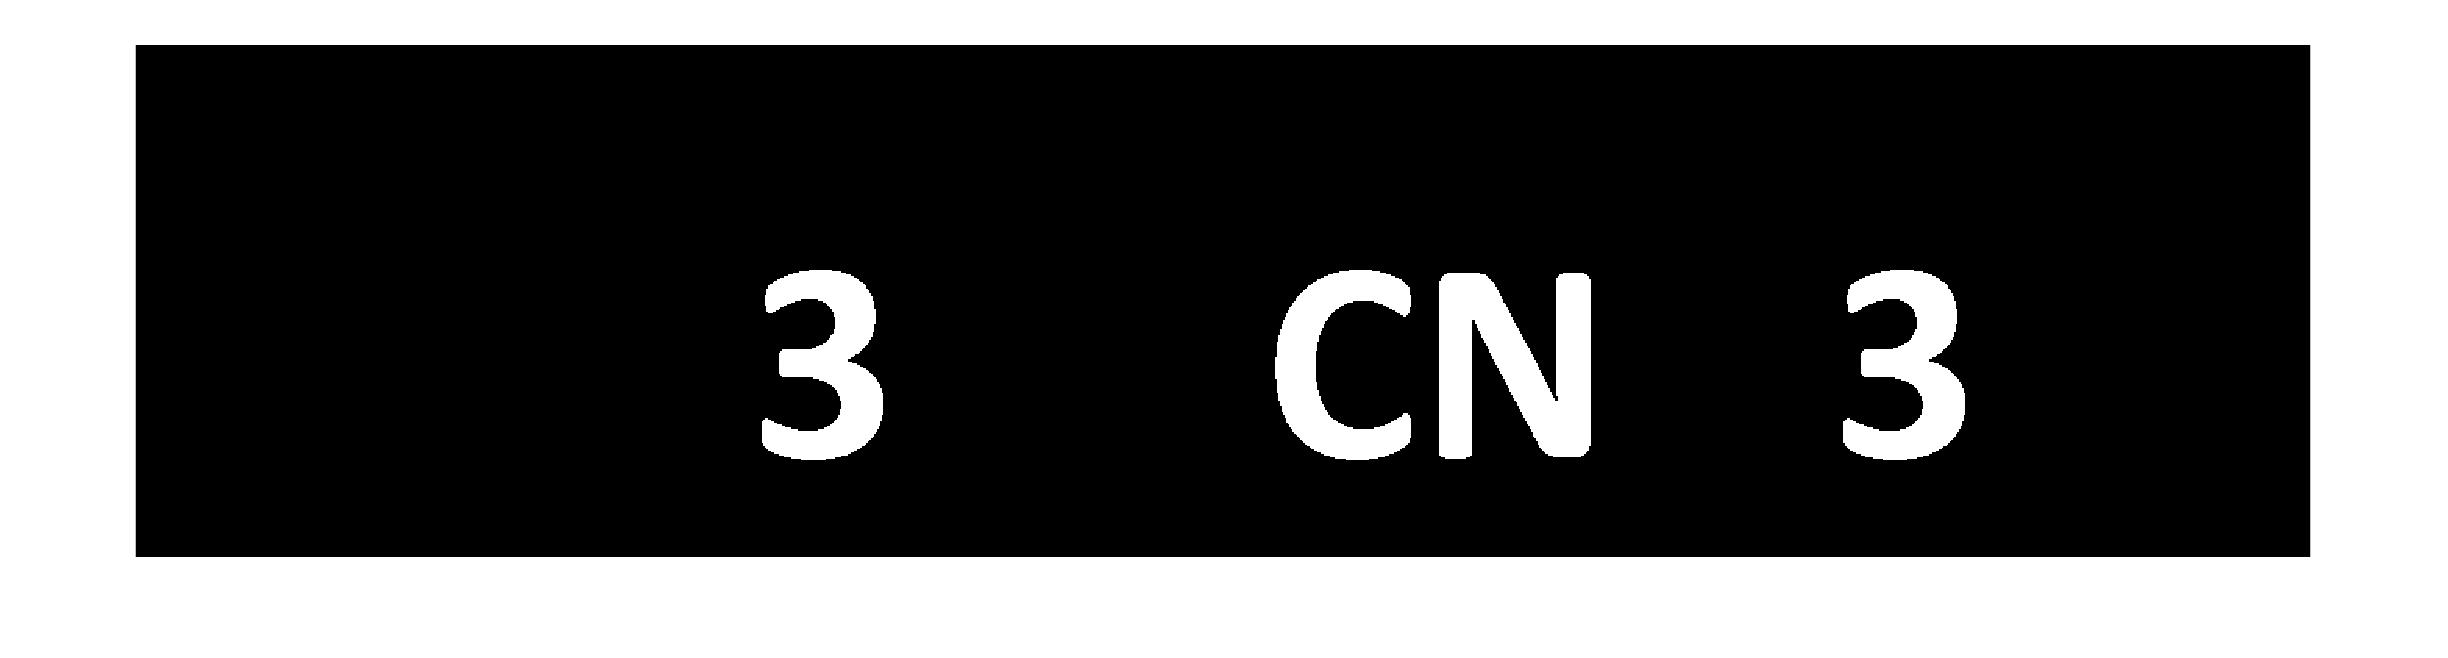
\includegraphics[height=1cm]{Results/Q2/NumPlate1/qanumber_plate_1Added3.jpg}}%
		\caption{Characters Extracted from Loops 1-3}
		\label{fig:}
	\end{figure}
	\begin{figure}[H]
		\centering
		\subcaptionbox{Loop 4 Result}
		[.3\linewidth]{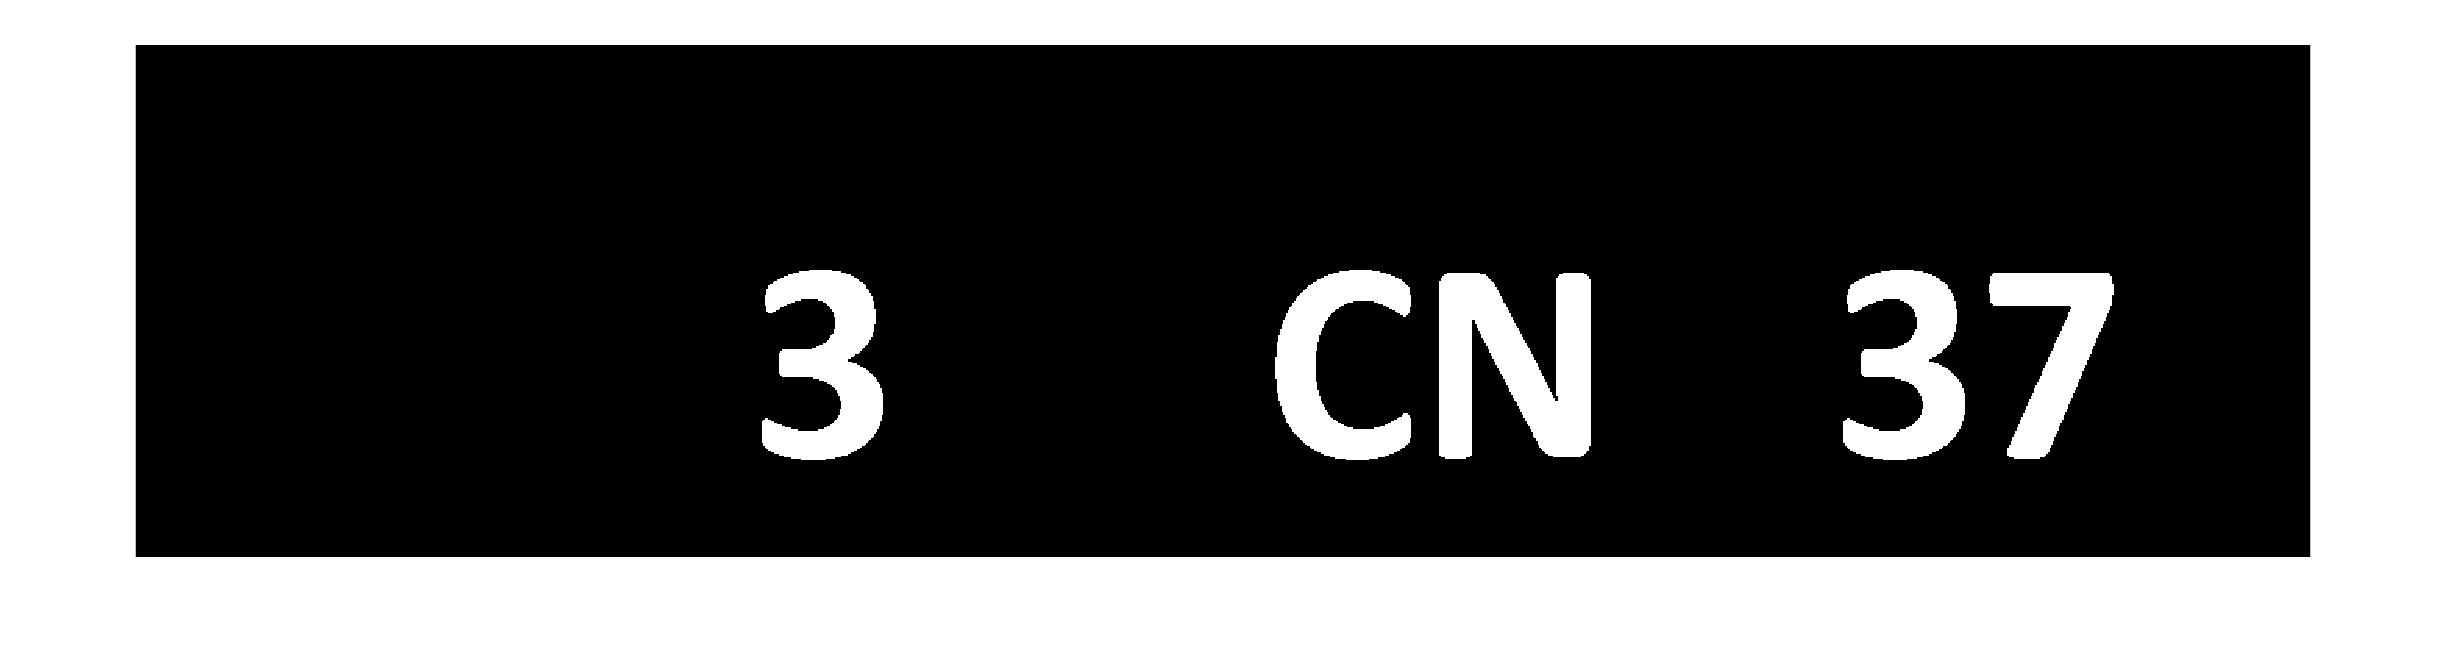
\includegraphics[height=1cm]{Results/Q2/NumPlate1/qanumber_plate_1Added4.jpg}}%
		\subcaptionbox{Loop 5 Result}
		[.3\linewidth]{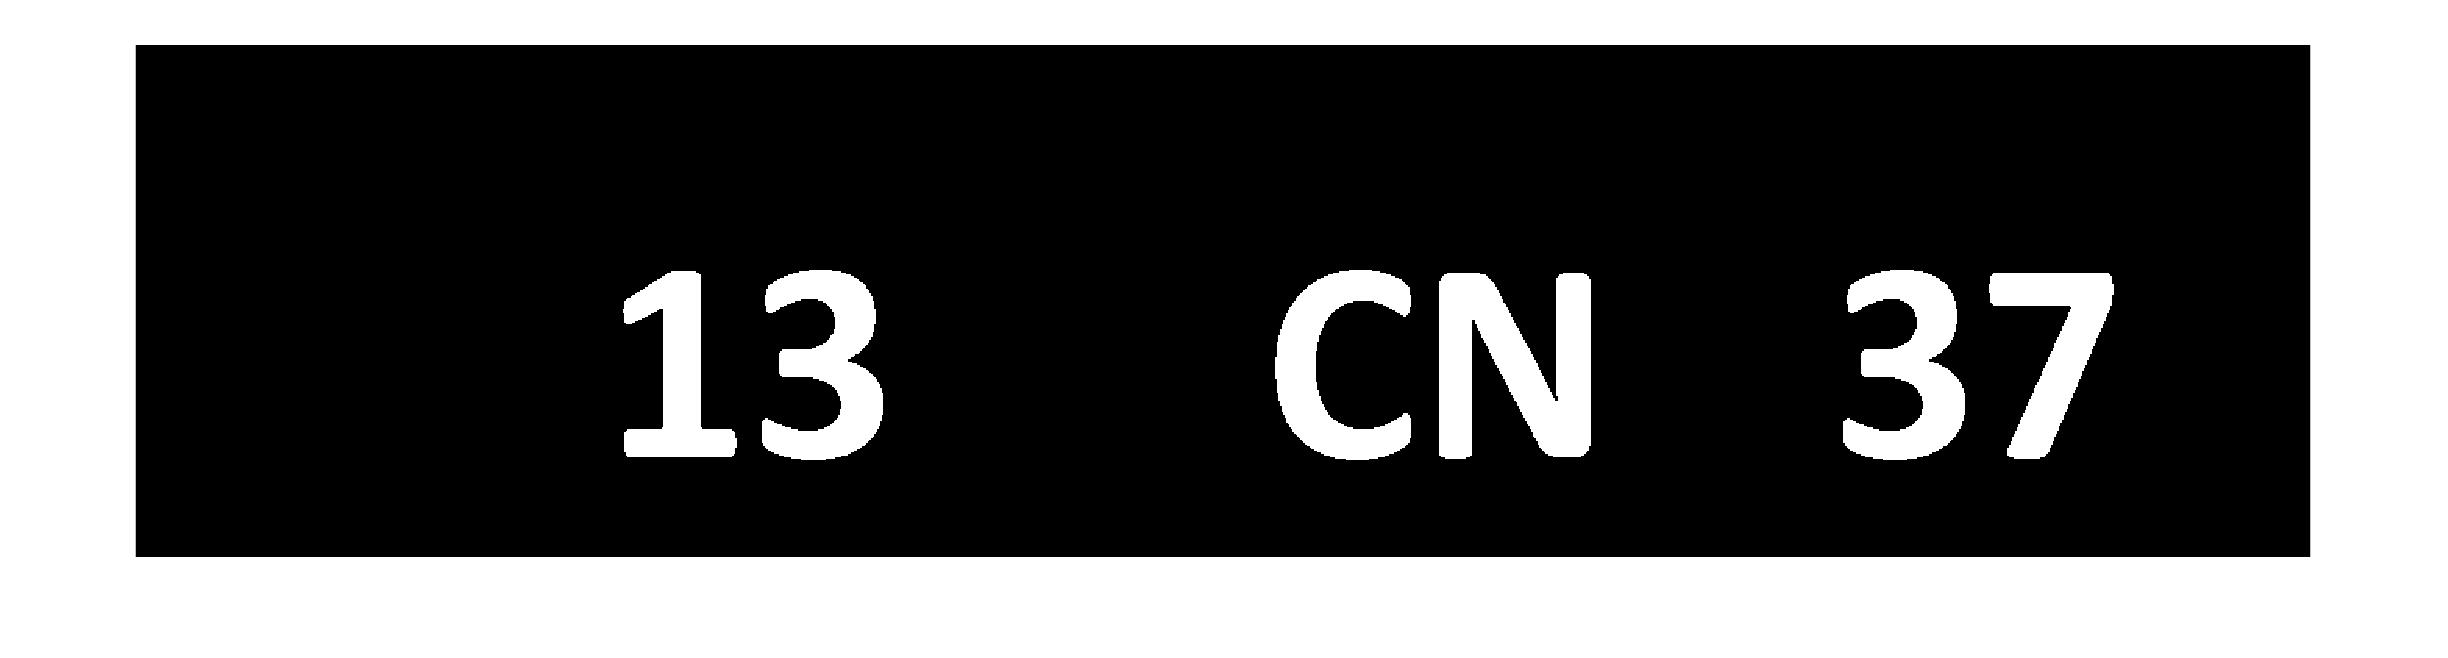
\includegraphics[height=1cm]{Results/Q2/NumPlate1/qanumber_plate_1Added5.jpg}}%
		\subcaptionbox{Loop 6 Result}
		[.3\linewidth]{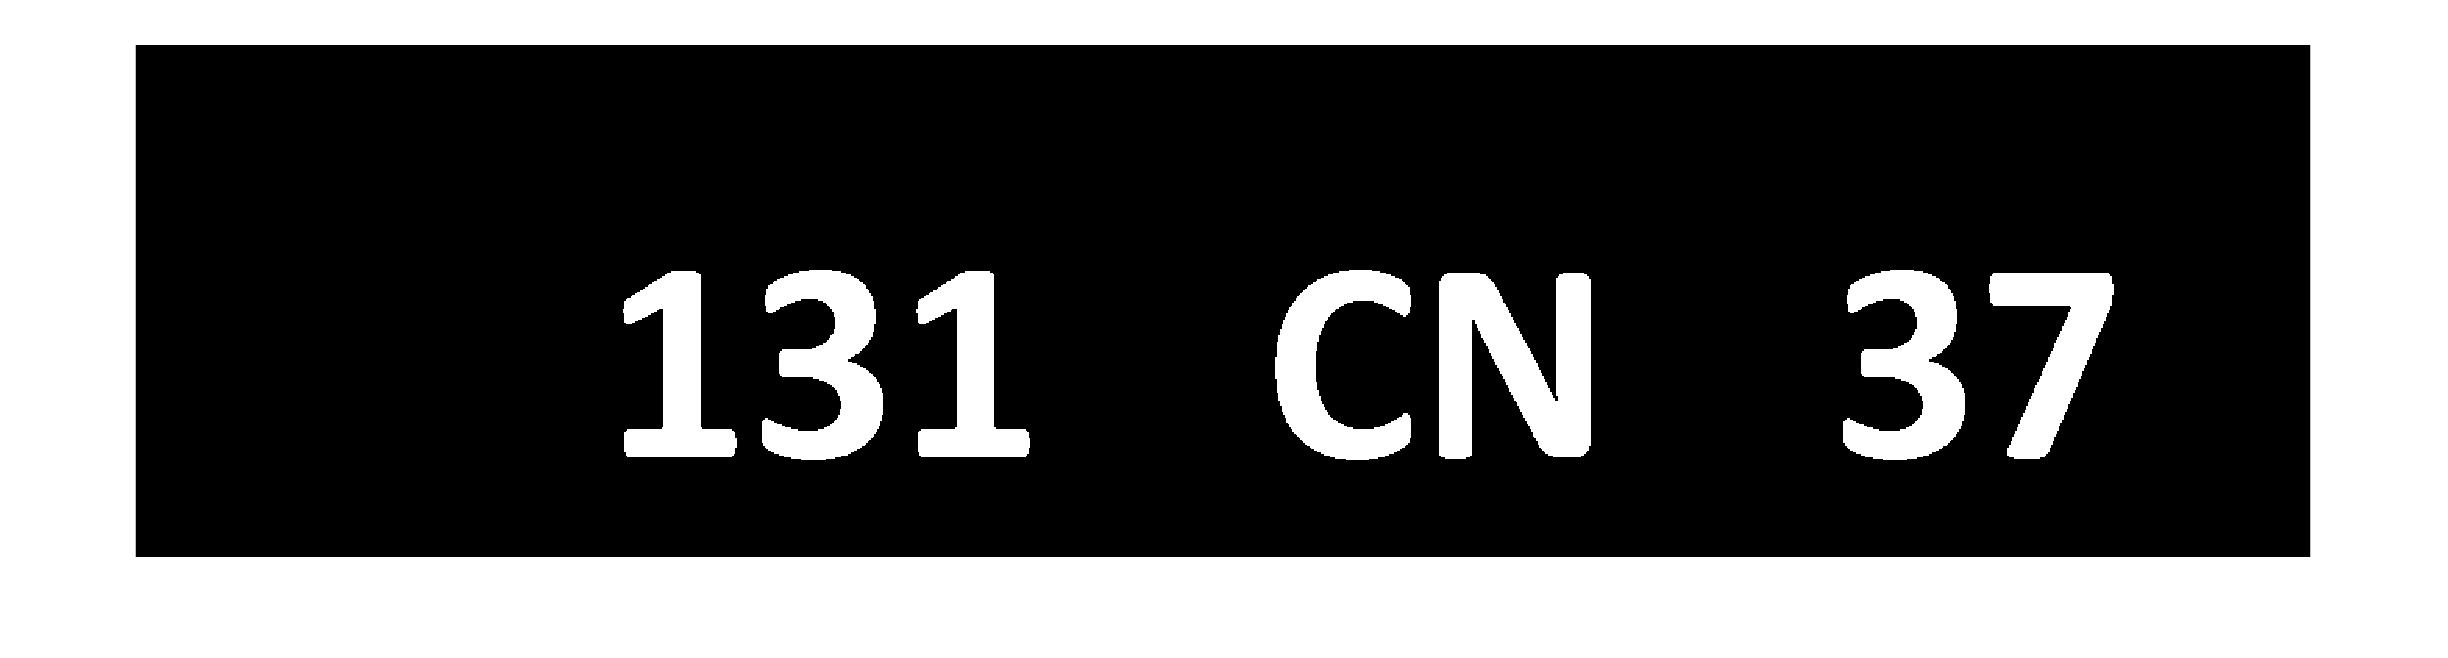
\includegraphics[height=1cm]{Results/Q2/NumPlate1/qanumber_plate_1Added6.jpg}}%
		\caption{Characters Extracted from Loops 4-6}
		\label{fig:}
	\end{figure}
	\begin{figure}[H]
		\centering
		\subcaptionbox{Canny Edge Detection}
		[.5\linewidth]{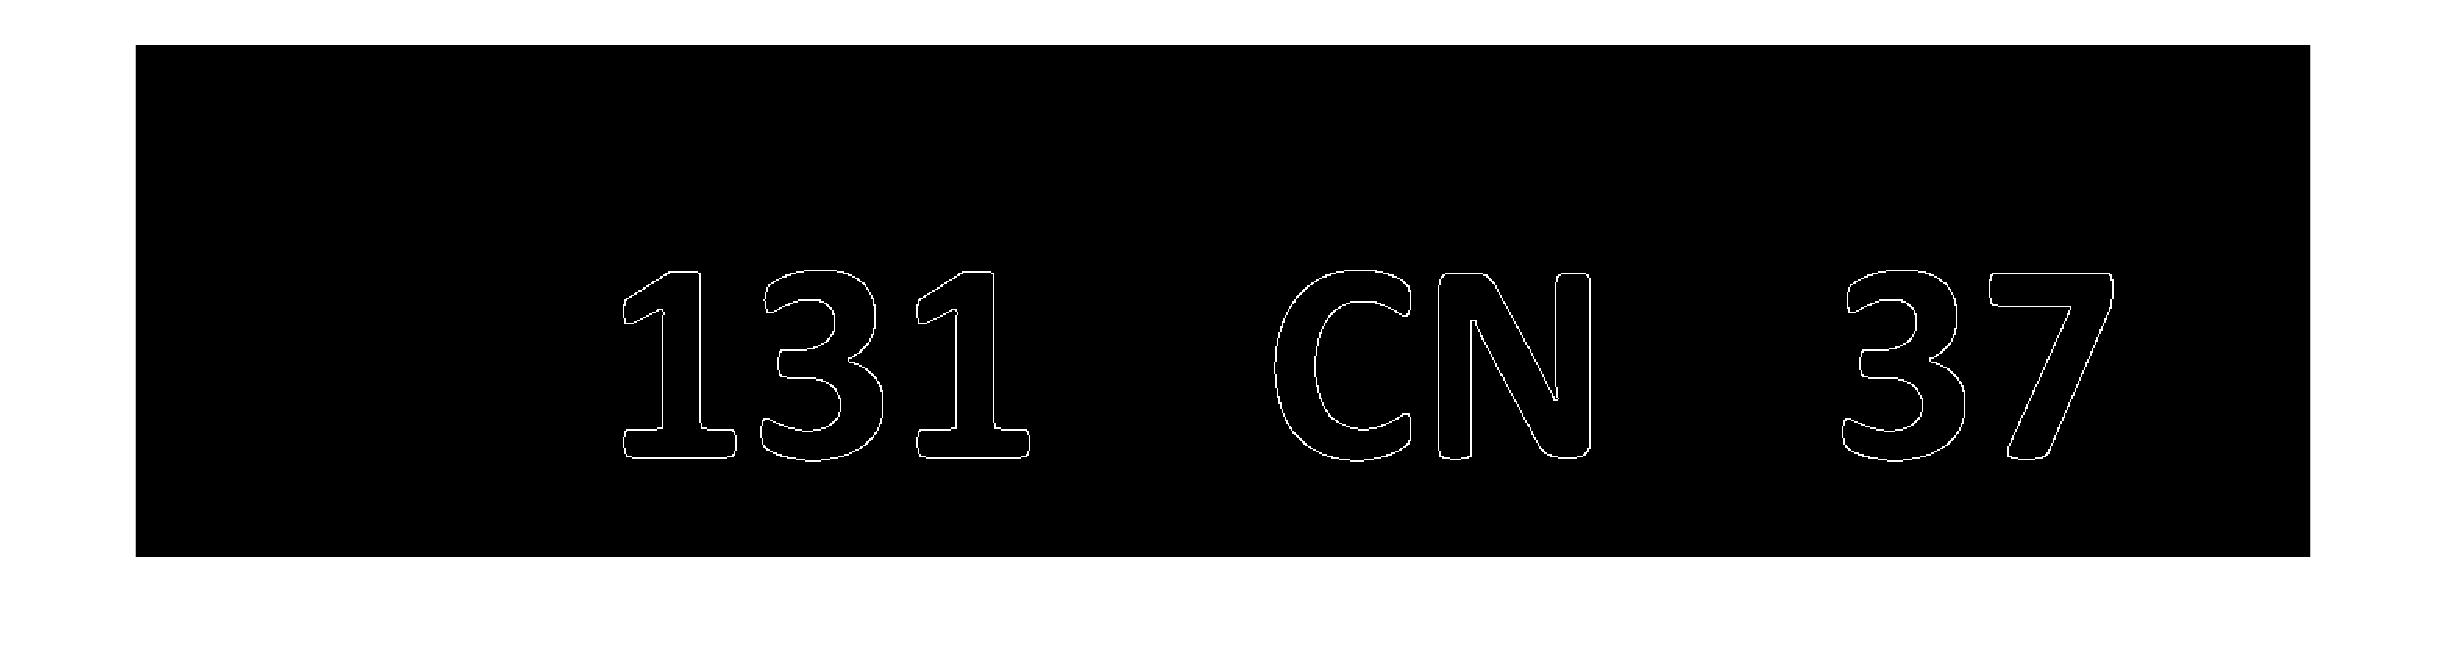
\includegraphics[height=1.5cm]{Results/Q2/NumPlate1/qanumber_plate_1Canny.jpg}}%
		\subcaptionbox{Overlayed Images}
		[.5\linewidth]{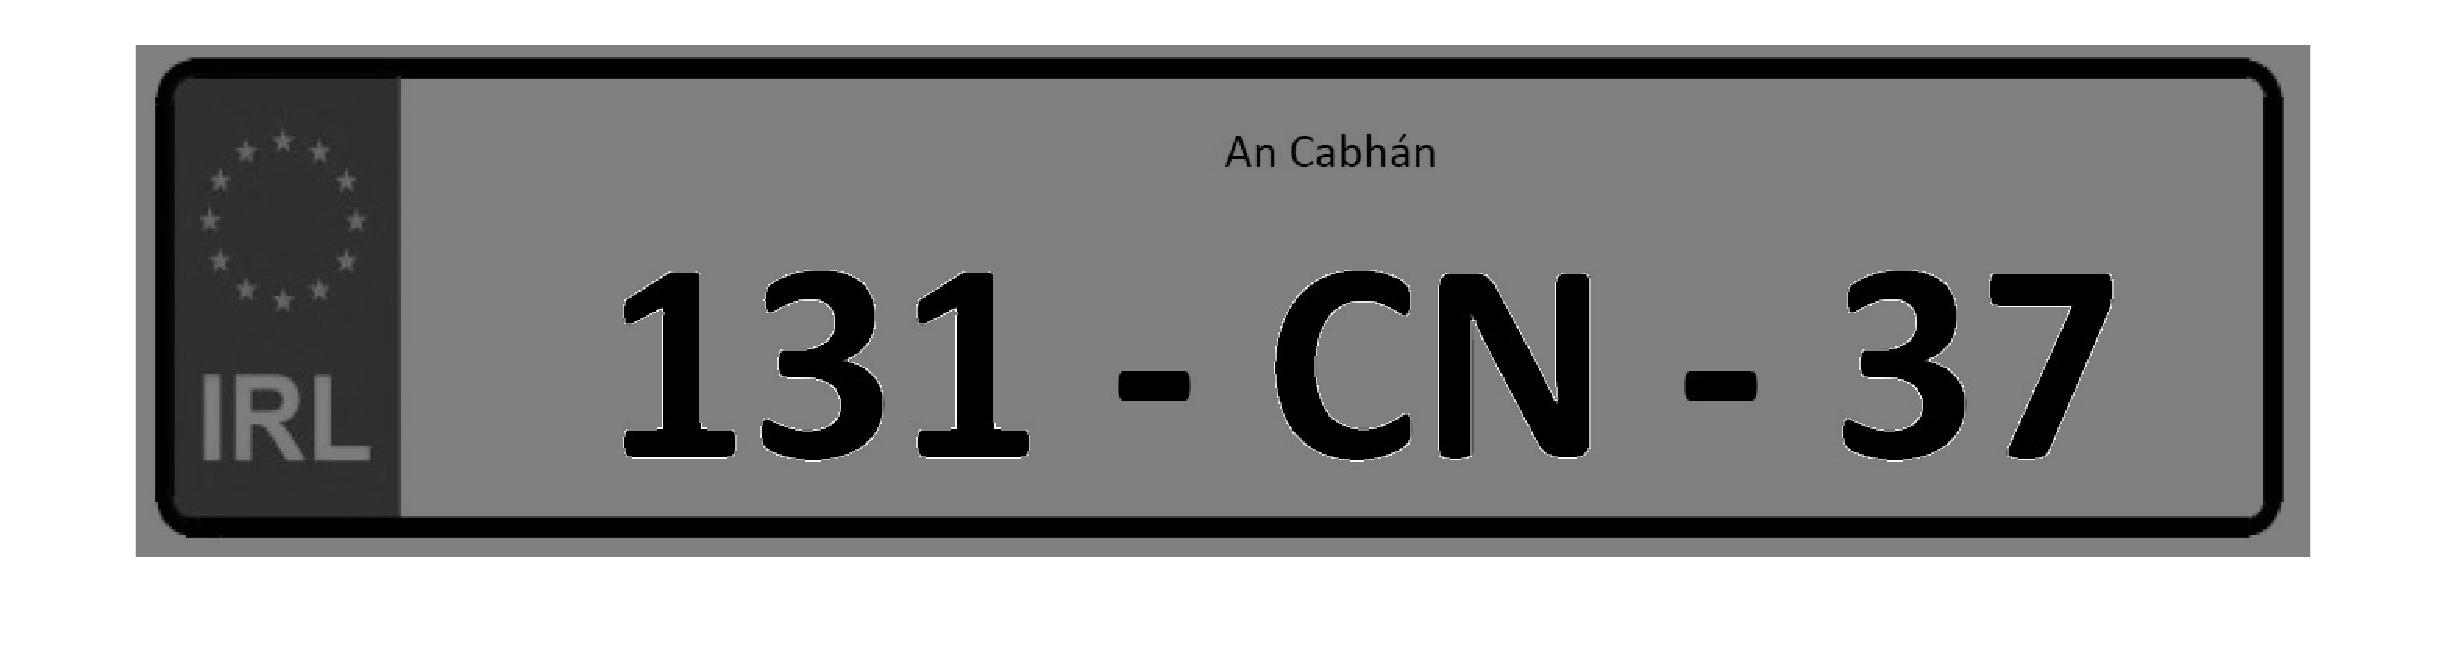
\includegraphics[height=1.5cm]{Results/Q2/NumPlate1/qanumber_plate_1Overlay.jpg}}%
		\caption{Overlayed Extracted Characters}
		\label{fig:}
	\end{figure}
	\par In order to test that this code is working as intended, a unit test file
	(q2patest.m) is executed. The original .m file is converted to a
	function, with the output being the number of characters found. An
	assertion within the unit test checks each test licence plate image
	against it's expected resulting number of characters.
	\subsubsection{Part b}
	In order to test that the robustness of this code, a unit test file
	(q2pbtest.m) is executed. An assertion within the unit test checks the
	licence plate image against it's expected resulting number of
	characters, while passing a variance value to the ``imnoise'' function.
	\par The point at which the solution fails is with a variance value of
	6. At this point, enough noise is added that the border blob which is
	extracted is split, leaving a blob which is then mistakenly extracted as
	a character in the registration. As such, the unit test fails, with an
	output value of (in the below case) 8 not matching the correct value of
	7.
	\begin{figure}[H]
		\centering
		\subcaptionbox{Zero Noise Overlay}
		[.5\linewidth]{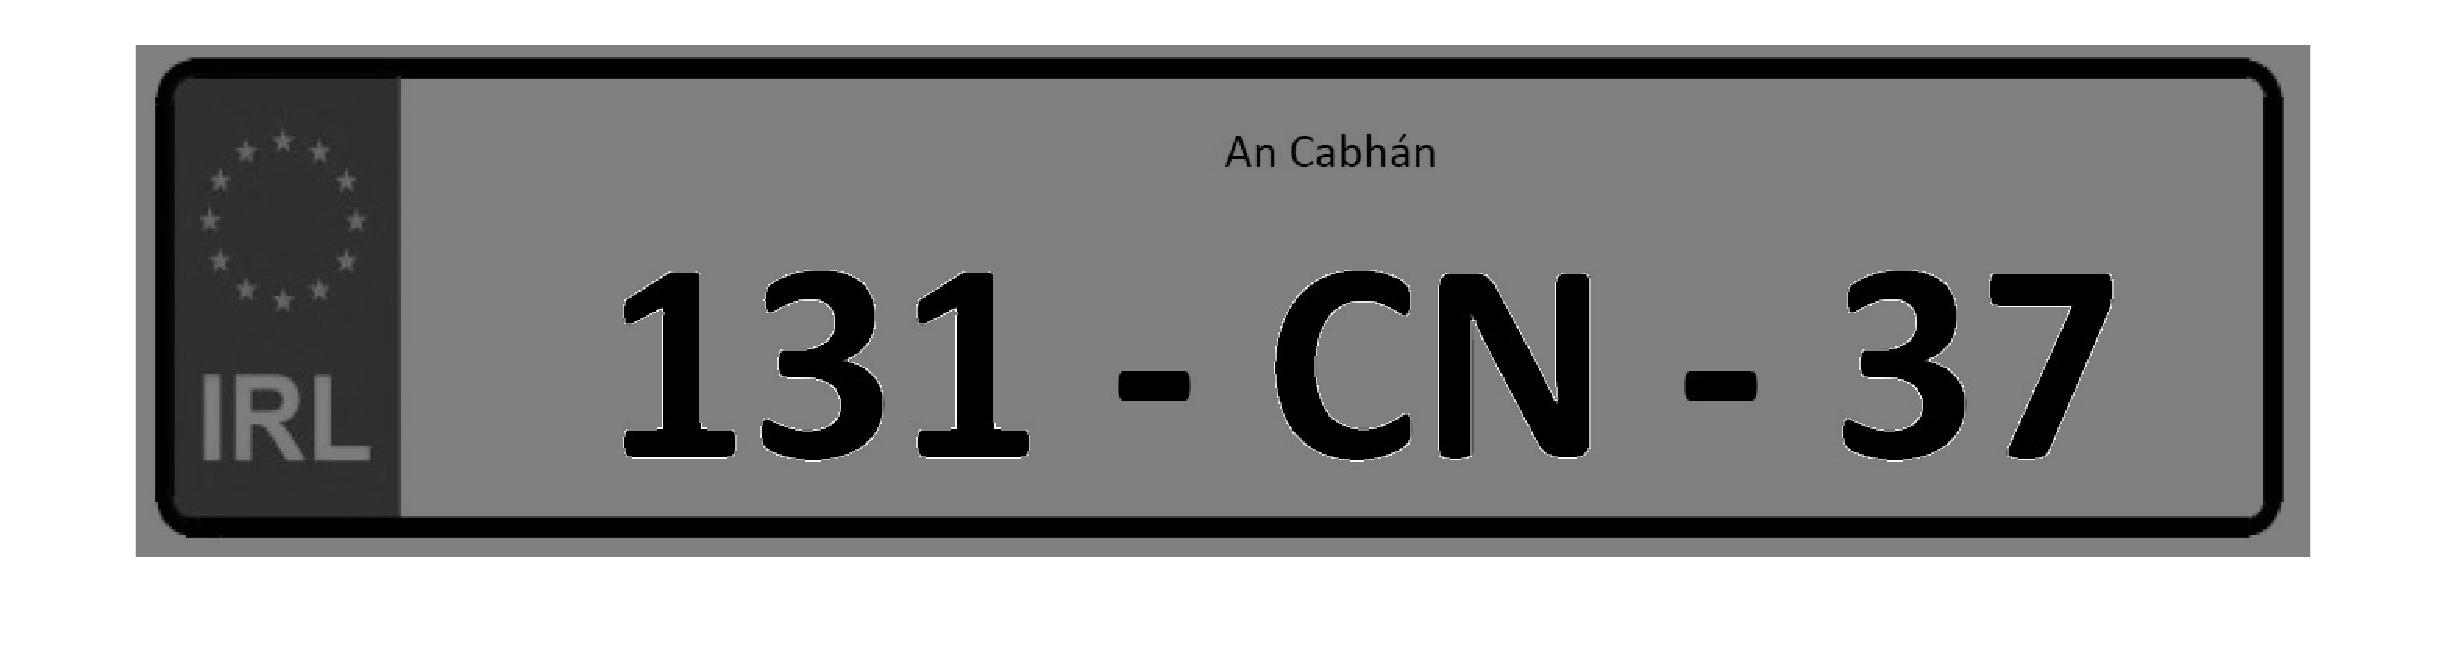
\includegraphics[height=1.5cm]{Results/Q2/NumPlate1/qanumber_plate_1Overlay.jpg}}%
		\subcaptionbox{Noise (with Variance 6) Overlay}
		[.5\linewidth]{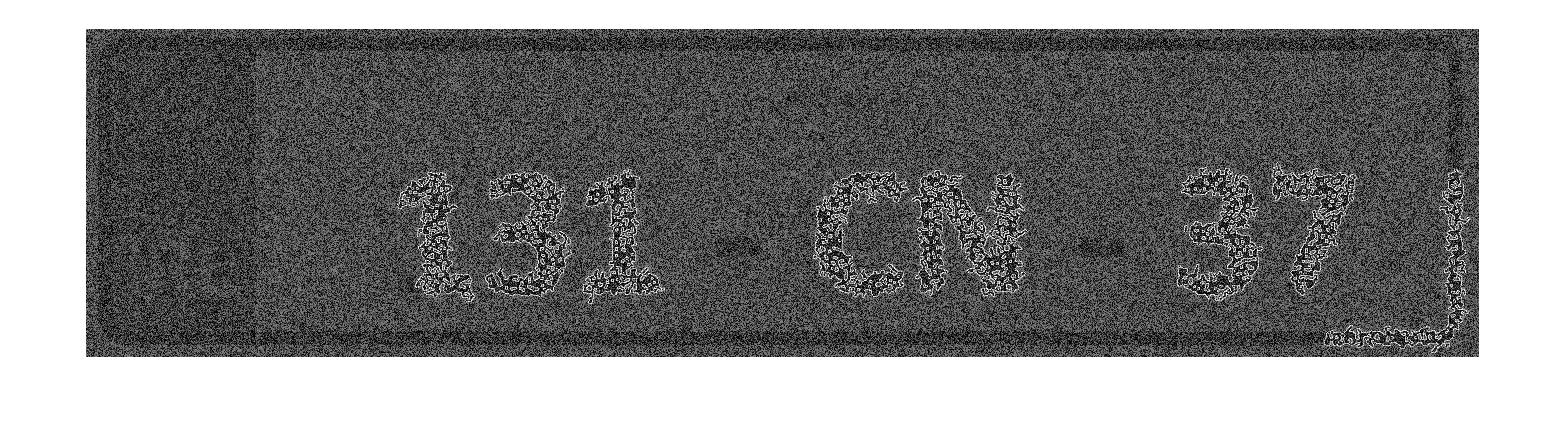
\includegraphics[height=1.5cm]{Results/Q2/noiseVar6Overlay.jpg}}%
		\caption{Overlayed Characters}
		\label{fig:}
	\end{figure}
	\subsection{Conclusion}
	The final workspace shows the input image format, dimensions $328 \times
	1393 \time 3$. This RGB image is converted to greyscale, removing the
	three channels for the colourspace.
	\begin{figure}[H]
		\centering
		\includegraphics[height=5cm]{Results/Q2/NumPlate6/Workspace.jpg}%
		\caption{Part a Workspace}
		\label{fig:}
	\end{figure}
	\par There are a number of intermediate values, of the same dimensions
	as the input image, used for the intermediate processing steps required
	in extracting the registration characters.
	\par These intermediate steps include the low pass filtering,
	thresholding, inversion, and biggest blob removal. The looping of
	biggest blob removal, and addition to the output image is also stored in
	one of these intermediate values.
	\par The chosen solution of looping through the biggest blobs until a
	certain ratio is reached allows for the robustness of this solution. An
	initial tested solution used the smallest blob in order to extract the
	characters, however, adding noise to the image increases the time taken
	to complete the task beyond the point of being usable.
	\par The code utilised in the completion of this section, along with the
	output images from each example, can be found within the Appendices.
	\section{Part 3: Convolution}
	\subsection{Introduction}
	Convolution is a common practice for pattern matching between an input
	image and a template image. In this section, a patterned input image,
	consisting of approximately 28 occurrences (full or partial) of the
	given template image, must have the number of full occurrences
	calculated.
	\par Greyscale convolution between the input image and the template must
	return the number of fully visible pattern matches (i.e. matches with
	features not in contact with the borders), in a way which us both
	robust, and data drive. By using dilation, the features touching the
	border can be removed, and the following features can be highlighted
	using a combination of centroid, point to square, and overlaying
	techniques.
	\subsection{Techniques}
	In completing this section of the assignment, the following techniques
	are utilised:
	\subsubsection{Part a}
	\underline{\textbf{Convolution}}
	\par Convolution is a template matching technique. A template mask is
	compared across an input image. A strong match between the template
	image and the input image is represented by a greater intensity value.
	The VSG ``Convolution'' function takes an input image and template, and
	returns an image, of type double, with the same dimensions as the input
	image.
	\par\underline{\textbf{Rotate}}
	\par Rotation is required both for testing the robustness of a solution, and
	for better template matching with respect to convolution. The VSG
	``RotateImg'' function rotates an input image by an input angle.
	\par\underline{\textbf{Centroid}}
	\par The centroid of an object is its center of gravity. This can be used
	within image processing for labelling purposes. The VSG ``Centroid''
	function places a single white pixel at the ``center of gravity'' of the
	white blobs within the image. The output of this function is an image of
	the same dimensions as the input image, with single white pixels (of
	value 255), surrounded by black pixels (of value 0).
	\par\underline{\textbf{Point to Square}}
	\par In order to more easily represent a functions output, points can be
	converted to larger, more visible features. The VSG ``Point2Square''
	function places a 5x5 square surrounding any single pixels of intensity
	value 255.
	\subsubsection{Part b}
	\underline{\textbf{Reconstruction By Dilation}}
	\par Reconstruction by dilation is a technique which can be used to
	detect features in contact with the image border. Passing the input
	image into the VSG ``ReconByDil'' function, along with the border pixels
	of the image, the features in contact with the border can be
	reconstructed, and subsequently removed from the image.
	\subsection{Pseudocode}
	\subsubsection{Part a}
	\begin{enumerate}
		\item Load the image into Matlab using the ``imread()''
			function.
		\item Use the ``rgb2gray()'' function to convert the image to
			greyscale.
		\item Load the template image into Matlab using the ``imread()''
			function.
		\item Use the ``rgb2gray()'' function to convert the image to
			greyscale.
		\item Use the VSG ``Rotate'' function to obtain a $180^\circ$ rotated
			copy of the template.
		\item Apply convolution on the greyscale input image, using the
			greyscale template image, using the VSG ``Convolution''
			funciton.
		\item Apply convolution on the greyscale input image, using the
			rotated greyscale template image, using the VSG
			``Convolution'' function.
		\item Add the resulting images from the convolution functions.
		\item Apply a data driven global threshold to the image using
			the ``Threshold'' function of the VSG toolbox.
		\item Apply the VSG ``Centroid'' function to the thresholded
			image to attain a point at the center of each blob.
		\item Use the ``Point2Square'' function of the VSG toolbox to
			turn each centroid point to a square, for ease of
			viewing in the overlayed display.
		\item Overlay the squares on the original image by adding the
			``Point2Square'' resulting image to the original input
			image, using the VSG ``Add'' function.
	\end{enumerate}
	\subsubsection{Part b}
	\begin{enumerate}
		\item Repeat the steps described in Part a.
		\item After the input image has been converted to greyscale, use
			the ``ReconByDil'' function to remove any parts of the image
			in contact with the edge.
		\item After the ``Centroid'' function is executed, add a call to
			the ``WPCounter'' function, to count the white pixels,
			thus giving the number of template matches within the
			image.
	\end{enumerate}
	\subsubsection{Part c}
	\begin{enumerate}
		\item Follow the steps in Part a.
		\item Apply Gaussian noise to the greyscale input image using
			the ``imnoise()'' function.
		\item Adjust the variance of the ``imnoise()'' function until
			the count of template matches is no longer correct.
	\end{enumerate}
	\subsection{Results}
	\subsubsection{Part a}
	In part a, the greyscale convolution is executed correctly, resulting in
	the highlighting of the matching patterns within the image. The input
	image is first correctly loaded into Matlab, and converted to greyscale.
	\begin{figure}[H]
		\centering
		\subcaptionbox{Input Image}
		[.5\linewidth]{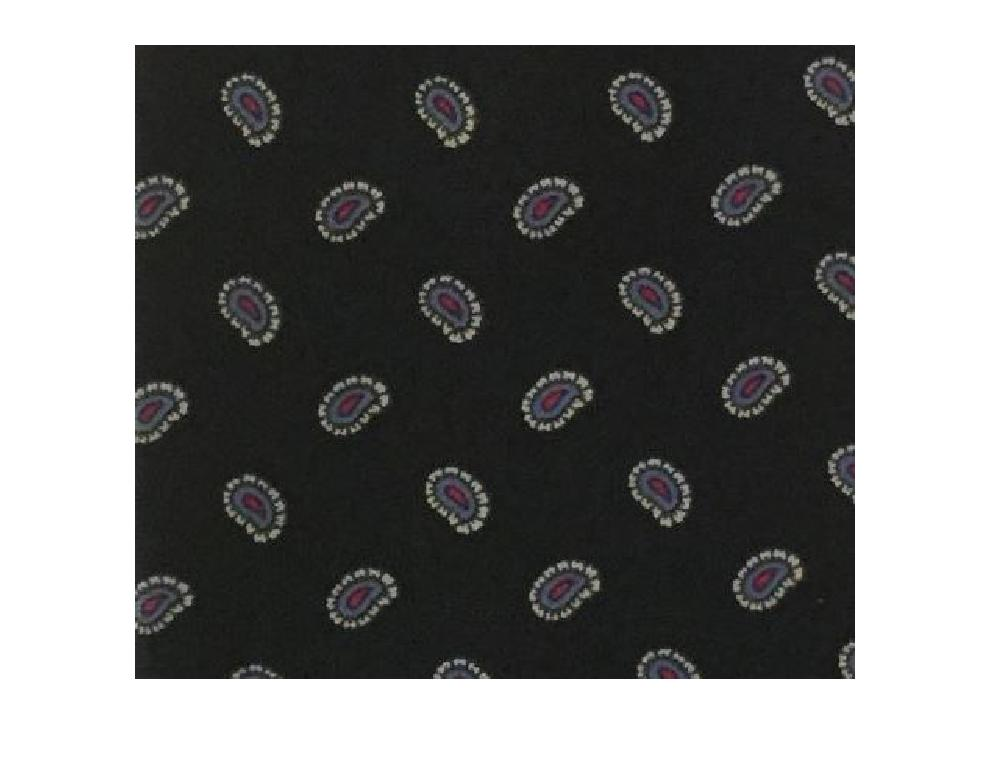
\includegraphics[height=5cm]{Results/Q3/a/qaInput.jpg}}%
		\subcaptionbox{Input Greyscale Image}
		[.5\linewidth]{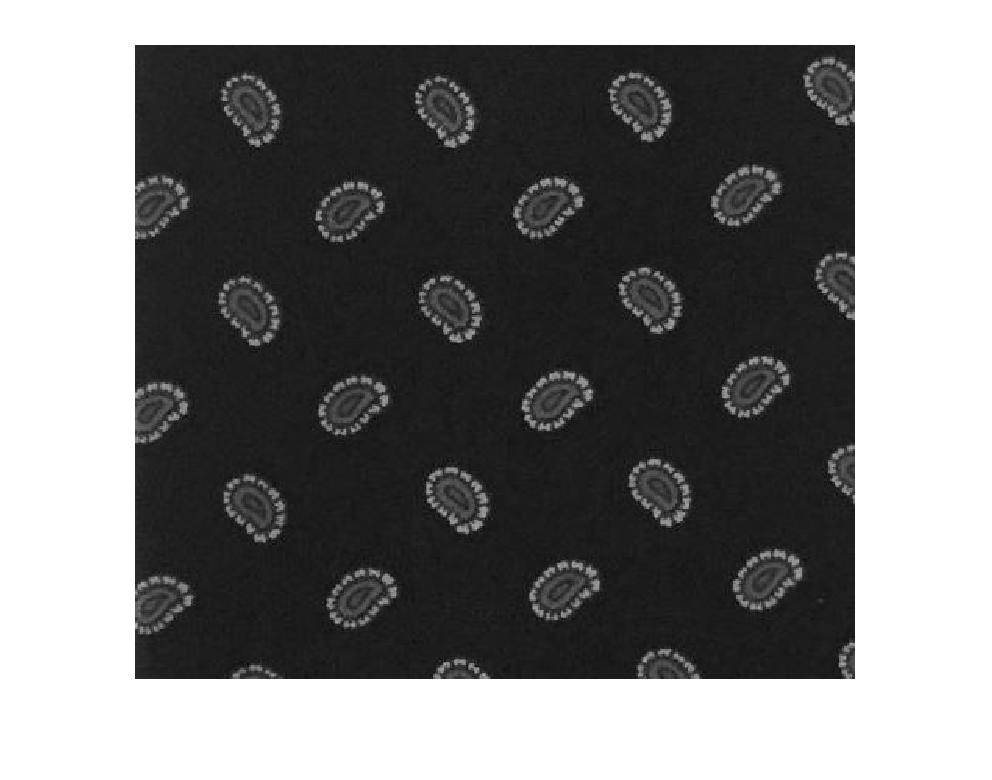
\includegraphics[height=5cm]{Results/Q3/a/qaInputGrey.jpg}}%
		\caption{Input image and Greyscale Conversion}
		\label{fig:}
	\end{figure}
	\par The template image is then loaded into Matlab, and is also
	converted to greyscale. In order to make the pattern matching more
	robust, a copy of the greyscale input is stored.
	\begin{figure}[H]
		\centering
		\subcaptionbox{Template Image}
		[.3\linewidth]{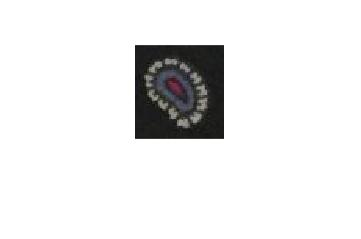
\includegraphics[height=3cm]{Results/Q3/a/qaTemplate.jpg}}%
		\subcaptionbox{Greyscale Template}
		[.3\linewidth]{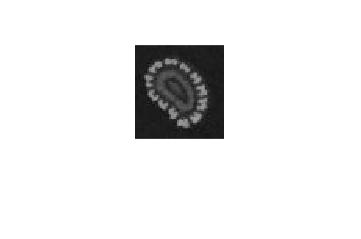
\includegraphics[height=3cm]{Results/Q3/a/qaTemplateGrey.jpg}}%
		\subcaptionbox{Template Rotated}
		[.3\linewidth]{\includegraphics[height=3cm]{Results/Q3/a/qaTemplateGreyRot.jpg}}%
		\caption{Required Template for Convolution}
		\label{fig:}
	\end{figure}
	\par The convolution function is applied to the input image with both
	the template, and rotated template images. The highlighted regions
	within the image is returned from the convolution function, and the two
	outputs are combined using the VSG ``Add'' function.
	\begin{figure}[H]
		\centering
		\subcaptionbox{Convolution (OT)}
		[.3\linewidth]{\includegraphics[height=3cm]{Results/Q3/a/qaConv.jpg}}%
		\subcaptionbox{Convolution (RT)}
		[.3\linewidth]{\includegraphics[height=3cm]{Results/Q3/a/qaConv2.jpg}}%
		\subcaptionbox{Convolution (+)}
		[.3\linewidth]{\includegraphics[height=3cm]{Results/Q3/a/qaAddedConv.jpg}}%
		\caption{Convolution outputs: Original Template(OT), Rotated
		Template(RT), Added Results(+)}
		\label{fig:}
	\end{figure}
	\par A data driven threshold, much like that used in section 1 is
	applied to the convolution output. This results in a number of blobs, of
	intensity value 255, which can then be converted to points using the
	``Centroid'' function. These points can be represented as squares for
	visualization purposes, using the ``Point2Square'' function.
	\begin{figure}[H]
		\centering
		\subcaptionbox{Threshold}
		[.3\linewidth]{\includegraphics[height=3cm]{Results/Q3/a/qaThresh.jpg}}%
		\subcaptionbox{Centroid}
		[.3\linewidth]{\includegraphics[height=3cm]{Results/Q3/a/qaCentroid.jpg}}%
		\subcaptionbox{Point2Square}
		[.3\linewidth]{\includegraphics[height=3cm]{Results/Q3/a/qaP2S.jpg}}%
		\caption{Outputs from the ``Threshold'', ``Centroid'', and
		``Point2Square'' Functions, showing the locations of template
	matches}
		\label{fig:}
	\end{figure}
	\par The squares representing the positions of pattern matches can be
	overlayed on the original image, using the VSG ``Add'' function.
	\begin{figure}[H]
		\centering
		\includegraphics[height=5cm]{Results/Q3/a/qaOverlay.jpg}%
		\caption{Overlay showing Location of Pattern Matches}
		\label{fig:}
	\end{figure}
	\par In order to investigate the effects of rotating the input image,
	the greyscale input image is rotated by 30, 45, and 60 degrees.
	\begin{figure}[H]
		\centering
		\subcaptionbox{Input $30^\circ$}
		[.3\linewidth]{\includegraphics[height=3cm]{Results/Q3/a/qaInputRot30.jpg}}%
		\subcaptionbox{Input $45^\circ$}
		[.3\linewidth]{\includegraphics[height=3cm]{Results/Q3/a/qaInputRot45.jpg}}%
		\subcaptionbox{Input $60\circ$}
		[.3\linewidth]{\includegraphics[height=3cm]{Results/Q3/a/qaInputRot60.jpg}}%
		\caption{Input Image Rotated $30^\circ, 45^\circ$ \& $60^\circ$}
		\label{fig:}
	\end{figure}
	Applying convolution with the two template images results in the
	following images.
	\begin{figure}[H]
		\centering
		\subcaptionbox{Convolution1 $30^\circ$}
		[.3\linewidth]{\includegraphics[height=3cm]{Results/Q3/a/qaConv1-30.jpg}}%
		\subcaptionbox{Convolution1 $45^\circ$}
		[.3\linewidth]{\includegraphics[height=3cm]{Results/Q3/a/qaConv1-45.jpg}}%
		\subcaptionbox{Convolution1 $60\circ$}
		[.3\linewidth]{\includegraphics[height=3cm]{Results/Q3/a/qaConv1-60.jpg}}%
		\caption{Convolution with Template: $30^\circ, 45^\circ$ \& $60^\circ$}
		\label{fig:}
	\end{figure}
	\begin{figure}[H]
		\centering
		\subcaptionbox{Convolution2 $30^\circ$}
		[.3\linewidth]{\includegraphics[height=3cm]{Results/Q3/a/qaConv2-30.jpg}}%
		\subcaptionbox{Convolution2 $45^\circ$}
		[.3\linewidth]{\includegraphics[height=3cm]{Results/Q3/a/qaConv2-45.jpg}}%
		\subcaptionbox{Convolution2 $60\circ$}
		[.3\linewidth]{\includegraphics[height=3cm]{Results/Q3/a/qaConv2-60.jpg}}%
		\caption{Convolution with Rotated Template: $30^\circ, 45^\circ$ \& $60^\circ$}
		\label{fig:}
	\end{figure}
	\par Adding the results of the convolutions results in the following
	images.
	\begin{figure}[H]
		\centering
		\subcaptionbox{Added Convolution $30^\circ$}
		[.3\linewidth]{\includegraphics[height=3cm]{Results/Q3/a/qaAddedConv30.jpg}}%
		\subcaptionbox{Added Convolution $45^\circ$}
		[.3\linewidth]{\includegraphics[height=3cm]{Results/Q3/a/qaAddedConv45.jpg}}%
		\subcaptionbox{Added Convolution $60\circ$}
		[.3\linewidth]{\includegraphics[height=3cm]{Results/Q3/a/qaAddedConv60.jpg}}%
		\caption{Added Convolution Results: $30^\circ, 45^\circ$ \& $60^\circ$}
		\label{fig:}
	\end{figure}
	\par Thresholding each of the convolution outputs returns a number of
	blobs, as in the original image, rotated by the input angle.
	\begin{figure}[H]
		\centering
		\subcaptionbox{Threshold $30^\circ$}
		[.3\linewidth]{\includegraphics[height=3cm]{Results/Q3/a/qaThresh30.jpg}}%
		\subcaptionbox{Threshold $45^\circ$}
		[.3\linewidth]{\includegraphics[height=3cm]{Results/Q3/a/qaThresh45.jpg}}%
		\subcaptionbox{Threshold $60\circ$}
		[.3\linewidth]{\includegraphics[height=3cm]{Results/Q3/a/qaThresh60.jpg}}%
		\caption{Threshold: $30^\circ, 45^\circ$ \& $60^\circ$}
		\label{fig:}
	\end{figure}
	\par The centroid of each blob in the resulting threshold image is shown
	below, with a single white pixel of intensity 255 representing the
	``center of gravity'' of the blob.
	\begin{figure}[H]
		\centering
		\subcaptionbox{Centroid $30^\circ$}
		[.3\linewidth]{\includegraphics[height=3cm]{Results/Q3/a/qaCentroid30.jpg}}%
		\subcaptionbox{Centroid $45^\circ$}
		[.3\linewidth]{\includegraphics[height=3cm]{Results/Q3/a/qaCentroid45.jpg}}%
		\subcaptionbox{Centroid $60\circ$}
		[.3\linewidth]{\includegraphics[height=3cm]{Results/Q3/a/qaCentroid60.jpg}}%
		\caption{Centroid: $30^\circ, 45^\circ$ \& $60^\circ$}
		\label{fig:}
	\end{figure}
	\par As before, the ``Point2Square'' function is used for visualisation
	purposes.
	\begin{figure}[H]
		\centering
		\subcaptionbox{Point2Square $30^\circ$}
		[.3\linewidth]{\includegraphics[height=3cm]{Results/Q3/a/qaP2S30.jpg}}%
		\subcaptionbox{Point2Square $45^\circ$}
		[.3\linewidth]{\includegraphics[height=3cm]{Results/Q3/a/qaP2S45.jpg}}%
		\subcaptionbox{Point2Square $60\circ$}
		[.3\linewidth]{\includegraphics[height=3cm]{Results/Q3/a/qaP2S60.jpg}}%
		\caption{Point2Square: $30^\circ, 45^\circ$ \& $60^\circ$}
		\label{fig:}
	\end{figure}
	\par The overlay images show the offset between the original input
	image (not rotated), and the template matches (rotated).
	\begin{figure}[H]
		\centering
		\subcaptionbox{Overlay $30^\circ$}
		[.3\linewidth]{\includegraphics[height=3cm]{Results/Q3/a/qaOverlay30.jpg}}%
		\subcaptionbox{Overlay $45^\circ$}
		[.3\linewidth]{\includegraphics[height=3cm]{Results/Q3/a/qaOverlay45.jpg}}%
		\subcaptionbox{Overlay $60\circ$}
		[.3\linewidth]{\includegraphics[height=3cm]{Results/Q3/a/qaOverlay60.jpg}}%
		\caption{Overlay: $30^\circ, 45^\circ$ \& $60^\circ$}
		\label{fig:}
	\end{figure}
	\par In order to evaluate the effects of varying the threshold value on
	the template matching, threshold functions of different values are
	applied to the convolution output. As can be seen, a lower threshold
	value of 32 results in a single blob, which would return a single
	centroid point and match.
	\par A threshold value of 50 results in a number of smaller unconnected
	blobs, which can give incorrect output values.
	\par A threshold value of 60 results in fewer blobs, therefore giving
	fewer centroids, and, again, incorrect output values.
	\begin{figure}[H]
		\centering
		\subcaptionbox{Threshold Value 32}
		[.3\linewidth]{\includegraphics[height=3cm]{Results/Q3/a/qaThreshVal32.jpg}}%
		\subcaptionbox{Threshold Value 50}
		[.3\linewidth]{\includegraphics[height=3cm]{Results/Q3/a/qaThreshVal50.jpg}}%
		\subcaptionbox{Threshold Value 60}
		[.3\linewidth]{\includegraphics[height=3cm]{Results/Q3/a/qaThreshVal60.jpg}}%
		\caption{Convolution Thresholded at Values: 32, 50, \& 60}
		\label{fig:}
	\end{figure}
	\subsubsection{Part b}
	\par In part b, the edge connected features are removed from the image
	using the VSG ``ReconByDil'' function, which, when given an input of the
	original images border pixels can ``regrow'' the connected features.
	These features can then be removed from the input image.
	\par The resulting image can then be processed as in part a.
	\begin{figure}[H]
		\centering
		\subcaptionbox{Dilated Image}
		[.3\linewidth]{\includegraphics[height=3cm]{Results/Q3/b/qbDilation.jpg}}%
		\subcaptionbox{Convolution}
		[.3\linewidth]{\includegraphics[height=3cm]{Results/Q3/b/qbConvolution.jpg}}%
		\subcaptionbox{Threshold}
		[.3\linewidth]{\includegraphics[height=3cm]{Results/Q3/b/qbThreshold.jpg}}%
		\caption{Dilation, Convolution and Thresholding Applied to Input
		Image}
		\label{fig:}
	\end{figure}
	\begin{figure}[H]
		\centering
		\subcaptionbox{Centroid}
		[.3\linewidth]{\includegraphics[height=3cm]{Results/Q3/b/qbCentroid.jpg}}%
		\subcaptionbox{Point2Square}
		[.3\linewidth]{\includegraphics[height=3cm]{Results/Q3/b/qbP2S.jpg}}%
		\subcaptionbox{Overlay}
		[.3\linewidth]{\includegraphics[height=3cm]{Results/Q3/b/qbOverlay.jpg}}%
		\caption{Overlay of Template Match on Original Input Image}
		\label{fig:}
	\end{figure}
	\par As visible in the above overlay image, the correct count of 18
	pattern matches is achieved.
	\subsubsection{Part c}
	\par Part c investigates the robustness of the chosen solution.
	Incrementing the noise variance shows that the incorrect pattern match
	count is achieved at a variance of 0.1, while the solution can deal with
	noise up to an approximate variance of 0.01.
	\begin{figure}[H]
		\centering
		\subcaptionbox{Noise Variance at 0.01}
		[.5\linewidth]{\includegraphics[height=5cm]{Results/Q3/c/qcOverlay001.jpg}}%
		\subcaptionbox{Noise Variance at 0.1}
		[.5\linewidth]{\includegraphics[height=5cm]{Results/Q3/c/qcOverlay01.jpg}}%
		\caption{Overlay showing correct template matching at 0.01
		variance, and incorrect matching at 0.1 variance.}
		\label{fig:}
	\end{figure}
	\subsection{Conclusion}
	The final workspace of part a shows the dimensions of the input RGB
	image ($406 \times 461 \times 3$), the input RGB mask ($60 \times 57
	\times 3$), and any intermediate values.
	 \par The greyscale input and mask images have the same dimensions as
	 the input images, however they do not have the channels for the
	 colourspace.
	 \par The final output image has all pattern matches, which includes
	 some incorrect matches due to the edge connected features, stored in an
	 RGB space, where the intensities of the squares used to represent the
	 pattern matches are added to the red channel of the original input
	 image.
	\begin{figure}[H]
		\centering
		\includegraphics[height=5cm]{Results/Q3/a/Workspace.jpg}%
		\caption{Part a Workspace}
		\label{fig:}
	\end{figure}
	\par The final workspace of part b shows the same values as in part a,
	alongside the ``numPatterns'' value, output from the ``WPCounter''
	function. This function counts the number of white pixels following the
	``Centroid'' function, which corresponds to the number of pattern
	matches in the image.
	\par As is required in the specification, there are 18 pattern matches
	found in the image.
	\begin{figure}[H]
		\centering
		\includegraphics[height=5cm]{Results/Q3/b/Workspace.jpg}%
		\caption{Part b Workspace}
		\label{fig:}
	\end{figure}
	The final workspace of part c shows the same values as in part b, with
	the newly completed dilation function output, and an incorrect output
	value for the number of pattern matches.
	\par As the noise applied to the input image is increased, the dilation
	begins to encroach further into the image than it should, affecting the
	pattern matches from the convolution function, which in turn affects the
	thresholding function. As such, adding noise to the image eventually results
	in an incorrect number of pattern matches.
	\begin{figure}[H]
		\centering
		\includegraphics[height=5cm]{Results/Q3/c/Workspace.jpg}%
		\caption{Part c Workspace}
		\label{fig:}
	\end{figure}
	\section{Appendix}
	\subsection{Part 1:}
	\subsubsection{Code:}
	\begin{lstlisting}[caption={Part 1 a}]
	% Setup Paths to VSG Toolbox and Local Data
addpath('C:\VSG_IPA_toolbox');
addpath('D:\Documents\College\Masters\Semester1\EE453-ImageProcessingAndAnalysis\Personal\Assignment');

% Clear workspace and free up system memory
clc
clear all

% Read Sample Image
A_COL = imread('face.jpg');
A_COL = uint8(vsg('Rotatep90', A_COL));
disp('Image read done');

% Display Image
h=figure;
imshow(uint8(A_COL));
set(h,'Name','Input Image');
saveas(h, 'Results\Q1\a\qaInput.jpg')

% Convert to greyscale and display the result
A=rgb2gray(A_COL);
h=figure;
imshow(uint8(A));
set(h,'Name','Greyscale Input');
saveas(h, 'Results\Q1\a\qaGreyscale.jpg')


% Wait for "Any key input" before deleting all figures
pause;
close all force;
\end{lstlisting}

\begin{lstlisting}[caption={Part 1 b}]
% Setup Paths to VSG Toolbox and Local Data
addpath('C:\VSG_IPA_toolbox');
addpath('D:\Documents\College\Masters\Semester1\EE453-ImageProcessingAndAnalysis\Personal\Assignment');

% Clear workspace and free up system memory
clc
clear all

% Read Sample Image
A_COL = imread('face.jpg');
A_COL = uint8(vsg('Rotatep90', A_COL));
disp('Image read done');

% Display Image
h=figure;
imshow(uint8(A_COL));
set(h,'Name','Input Image');

% Convert to greyscale and display the result
A=rgb2gray(A_COL);
h=figure;
imshow(uint8(A));
set(h,'Name','Greyscale Input');

% Data driven threshold based on the max/min of the image histogram
hi_grey=vsg('HighestGrey',A);
disp('Highestgrey done');
lo_grey=vsg('LowestGrey',A);
disp('Lowestgrey done');
thresh=uint8(3*(hi_grey+lo_grey)/4);

% Output the calculated threshold to the command window
string=['Data driven threshold is ' num2str(thresh)];
disp(string);

% Apply a fixed global threshold to the image and display the resultant binary image
C=vsg('Threshold',A,thresh);
h=figure;
imshow(uint8(C));
set(h,'Name','Threshold Data Drive');
saveas(h, 'Results\Q1\b\qbThreshData.jpg')

D=vsg('Threshold',A,125);
h=figure;
imshow(uint8(D));
set(h,'Name','Threshold 125');
saveas(h, 'Results\Q1\b\qbThresh125.jpg')

E=vsg('Threshold',A,130);
h=figure;
imshow(uint8(E));
set(h,'Name','Threshold 130');
saveas(h, 'Results\Q1\b\qbThresh130.jpg')

F=vsg('Threshold',A,140);
h=figure;
imshow(uint8(F));
set(h,'Name','Threshold 140');
saveas(h, 'Results\Q1\b\qbThresh140.jpg')

disp('Threshold done');
h=figure;
subplot(2,2,1), imshow(uint8(C));
subplot(2,2,2), imshow(uint8(D));
subplot(2,2,3), imshow(uint8(E));
subplot(2,2,4), imshow(uint8(F));
set(h,'Name','Threshold Image');

% Wait for "Any keey input" before deleting all figures
pause;
close all force;
\end{lstlisting}

\begin{lstlisting}[caption={Part 1 c}]
% Setup Paths to VSG Toolbox and Local Data
addpath('C:\VSG_IPA_toolbox');
addpath('D:\Documents\College\Masters\Semester1\EE453-ImageProcessingAndAnalysis\Personal\Assignment');

% Clear workspace and free up system memory
clc
clear all

% Read Sample Image
A_COL = imread('face.jpg');
A_COL = uint8(vsg('Rotatep90', A_COL));
disp('Image read done');

% Display Image
h=figure;
imshow(uint8(A_COL));
set(h,'Name','Input Image');

% Convert to greyscale and display the result
A=rgb2gray(A_COL);
h=figure;
imshow(uint8(A));
set(h,'Name','Greyscale Input');

F=vsg('5x5Thresh',A,0);
h=figure;
imshow(uint8(F))
set(h,'Name','5x5 Threshold');
saveas(h, 'Results\Q1\c\qcThresh5x5.jpg')

% Wait for "Any keey input" before deleting all figures
pause;
close all force;
\end{lstlisting}

\begin{lstlisting}[caption={Part 1 d}]
% Setup Paths to VSG Toolbox and Local Data
addpath('C:\VSG_IPA_toolbox');
addpath('D:\Documents\College\Masters\Semester1\EE453-ImageProcessingAndAnalysis\Personal\Assignment');

% Clear workspace and free up system memory
clc
clear all

% Read Sample Image
A_COL = imread('face.jpg');
A_COL = uint8(vsg('Rotatep90', A_COL));
disp('Image read done');

% Display Image
h=figure;
imshow(uint8(A_COL));
set(h,'Name','Input Image');

% Convert to greyscale and display the result
A=rgb2gray(A_COL);
h=figure;
imshow(uint8(A));
set(h,'Name','Greyscale Input');

i=.0001;
while i<10
    noiseFileName = strcat('Results\Q1\d\qdVar', num2str(i), '.jpg');
    ThreshFileName = strcat('Results\Q1\d\qdThresh', num2str(i), '.jpg');
    FiveThreshFileName = strcat('Results\Q1\d\qd5x5', num2str(i), '.jpg');

    B = imnoise(A, 'gaussian', 0, i);
    h=figure;
    imshow(uint8(B))
    set(h,'Name',noiseFileName);
    saveas(h, noiseFileName)

    % Apply the threshold to the image and display the resultant binary image
    E=vsg('Threshold',B,125);
    disp('Threshold done');
    h=figure;
    imshow(uint8(E));
    set(h,'Name','Threshold Image');
    saveas(h, ThreshFileName)

    % Mask boundary pixels to avoid any edge effects
    E=vsg('MaskImg',E,5);

    F=vsg('5x5Thresh',B,0);
    h=figure;
    imshow(uint8(F))
    saveas(h, FiveThreshFileName)


    i=i*10;
end;

% Wait for "Any key input" before deleting all figures
pause;
close all force;
\end{lstlisting}
	\subsection{Part 2:}
	\subsubsection{Code:}
\begin{lstlisting}[caption={Part 2 a}]
	% Setup Paths to VSG Toolbox and Local Data
addpath('C:\VSG_IPA_toolbox');
addpath('D:\Documents\College\Masters\Semester1\EE453-ImageProcessingAndAnalysis\Personal\Assignment');

% Clear workspace and free up system memory
clc
clear all

i=1;
inputImage = 'number_plate_1';
saveDirectory = 'NumPlate1';
inputFileName = strcat('data\', inputImage, '.jpg');
saveFileName = strcat('Results\Q2\', saveDirectory, '\qa', inputImage , '.jpg');
greyFileName = strcat('Results\Q2\', saveDirectory, '\qa', inputImage , 'Grey.jpg');
lowFileName = strcat('Results\Q2\', saveDirectory, '\qa', inputImage , 'Low.jpg');
midFileName = strcat('Results\Q2\', saveDirectory, '\qa', inputImage , 'Mid.jpg');
notFileName = strcat('Results\Q2\', saveDirectory, '\qa', inputImage , 'Not.jpg');
borderFileName = strcat('Results\Q2\', saveDirectory, '\qa', inputImage , 'Border.jpg');
noBorderFileName = strcat('Results\Q2\', saveDirectory ,'\qa', inputImage , 'NoBorder.jpg');
bigCharFileName = strcat('Results\Q2\', saveDirectory ,'\qa', inputImage , 'BigChar.jpg');
remainCharsFileName = strcat('Results\Q2\', saveDirectory ,'\qa', inputImage , 'Remain.jpg');
addedCharFileName = strcat('Results\Q2\', saveDirectory ,'\qa', inputImage , 'Added', num2str(i), '.jpg');
cannyFileName = strcat('Results\Q2\', saveDirectory ,'\qa', inputImage , 'Canny.jpg');
overlayFileName = strcat('Results\Q2\', saveDirectory ,'\qa', inputImage , 'Overlay.jpg');

% Read Sample Image
input_col = imread(inputFileName);
disp('Image read done');

% Display Image
h=figure;
imshow(uint8(input_col));
set(h,'Name','Input Image');
saveas(h, saveFileName)


% Convert to greyscale and display the result
in_img=rgb2gray(input_col);
h=figure;
imshow(uint8(in_img));
set(h,'Name','Greyscale Input');
saveas(h, greyFileName)


% Remove number plate border
[out_img1]=vsg('LowPass', in_img);
h=figure;
imshow(uint8(out_img1));
set(h,'Name','Low Pass Filtered Image');
saveas(h, lowFileName)

[out_img2]=vsg('MidThresh',out_img1);
h=figure;
imshow(uint8(out_img2));
set(h,'Name','MidThreshold Image');
saveas(h, midFileName)

[out_img3]=vsg('NOT',out_img2);
h=figure;
imshow(uint8(out_img3));
set(h,'Name','Inverted (NOT) Image');
saveas(h, notFileName)

[out_img4]=vsg('BiggestBlob',out_img3);
disp('BiggestBlob done');
%F=uint8(F);
h=figure;
imshow(uint8(out_img4));
set(h,'Name','BiggestBlob Image');
saveas(h, borderFileName)

[out_img5] = vsg('Subtract', out_img3, out_img4);
h=figure;
imshow(uint8(out_img5));
set(h,'Name','Subtracted Biggest Blob Image');
saveas(h, noBorderFileName)

% Extract number plate numbers
[out_img6] = vsg('BiggestBlob', out_img5);
h=figure;
imshow(uint8(out_img6));
set(h,'Name','Biggest Blob Image');
saveas(h, bigCharFileName)
[biggestBlobCounter] = vsg('WPCounter', uint8(out_img6))

[out_img5]=vsg('XOR', out_img5, out_img6);
% Remove 1 pixel white border from image.
[out_img5]=vsg('MaskImg', out_img5, 1);
h=figure;
imshow(uint8(out_img5));
saveas(h, remainCharsFileName)

while(vsg('WPCounter', vsg('BiggestBlob', out_img5))>(biggestBlobCounter/3))
  [tempBlob]=vsg('BiggestBlob', out_img5);
  h=figure;
  imshow(uint8(tempBlob));
  set(h,'Name','tempBlob');
  [biggestBlobCounter] = vsg('WPCounter', uint8(tempBlob))
  [out_img6]=vsg('XOR', out_img6, tempBlob);
  h=figure;
  imshow(uint8(out_img6));
  addedCharFileName = strcat('Results\Q2\', saveDirectory ,'\qa', inputImage , 'Added', num2str(i), '.jpg');
  saveas(h, addedCharFileName)
  set(h,'Name','Remaining Blobs Image');
  [out_img5]=vsg('Subtract', out_img5, tempBlob);
  i=i+1;
end
% Count number of blobs in the image
% Corresponds to the number of digits on the number plate
[numBlobs] = vsg('CountBlobs', uint8(out_img6));
disp(numBlobs);

% Overlay the identified number plate numbers on
% the original input image
[out_img7, out_img8]=vsg('Canny', out_img6,  1.0, 5, 200);
h=figure;
imshow(uint8(out_img7));
set(h,'Name','Edge Detector Image');
saveas(h, cannyFileName)

[out_img9] = vsg('Add', out_img7, in_img);
h=figure;
imshow(uint8(out_img9));
set(h,'Name','Overlayed (Add) Image');
saveas(h, overlayFileName)

% Wait for "Any key input" before deleting all figures
pause;
close all force;
\end{lstlisting}

\begin{lstlisting}[caption={Part 2 b - Functions used to reduce lines of code}]
function numBlobs = p2qb(im_path, noise_var)

% Setup Paths to VSG Toolbox and Local Data
addpath('C:\VSG_IPA_toolbox');
addpath('D:\Documents\College\Masters\Semester1\EE453-ImageProcessingAndAnalysis\Personal\Assignment');

% Clear workspace and free up system memory
%clc
%clear all


% Read Sample Image
input_col = imread(im_path);
disp('Image read done');

input_noisy = imnoise(input_col, 'gaussian', 0, noise_var);


% Display Image
% h=figure;
% imshow(uint8(input_col));
% set(h,'Name','Input Image');

% Convert to greyscale and display the result
in_img=rgb2gray(input_noisy);
% h=figure;
% imshow(uint8(in_img));
% set(h,'Name','Greyscale Input');

% Call Function to remove number plate border
[out_img1]=q2RemoveNumPlateBorder(in_img);

% Call Function to extract number plate numbers
[out_img2]=q2ExtractNumPlateNumbers(out_img1);

% Count number of blobs in the image
% Corresponds to the number of digits on the number plate
[numBlobs] = vsg('CountBlobs', uint8(out_img2));
disp(numBlobs);

% Overlay the identified number plate numbers on
% the original input image
[out_img3]=q2Overlay(out_img2, in_img);

% Wait for "Any key input" before deleting all figures
pause;
close all force;
end
\end{lstlisting}

\begin{lstlisting}[caption={Part 2 a Unit Test}]
clc;

%% Test Image 1

clear all;
assert(p2qa('data/number_plate_1.jpg')==7, 'Error in Output');

%% Test Image 2

clear all;
assert(p2qa('data/number_plate_2.jpg')==7, 'Error in Output');

%% Test Image 3

clear all;
assert(p2qa('data/number_plate_3.jpg')==6, 'Error in Output');

%% Test Image 4

clear all;
assert(p2qa('data/number_plate_4.jpg')==8, 'Error in Output');

%% Test Image 5

clear all;
assert(p2qa('data/number_plate_5.jpg')==7, 'Error in Output');

%% Test Image 6

clear all;
assert(p2qa('data/number_plate_6.jpg')==7, 'Error in Output');

\end{lstlisting}

\begin{lstlisting}[caption={Part 2 b Unit Test}]
clc
clear all

%% Test 1
i = 6;
assert(p2qb('data/number_plate_1.jpg', i)==7, 'Error in Output')
\end{lstlisting}
	\subsubsection{Images:}
	\begin{figure}[H]
		\centering
		\subcaptionbox{Input Image}
		[.3\linewidth]{\includegraphics[height=1cm]{Results/Q2/NumPlate2/qanumber_plate_2.jpg}}%
		\subcaptionbox{Greyscale Image}
		[.3\linewidth]{\includegraphics[height=1cm]{Results/Q2/NumPlate2/qanumber_plate_2Grey.jpg}}%
		\subcaptionbox{Low Pass Filtered}
		[.3\linewidth]{\includegraphics[height=1cm]{Results/Q2/NumPlate2/qanumber_plate_2Low.jpg}}%
		\caption{Initial Segmentation Setup}
		\label{fig:}
	\end{figure}
	\begin{figure}[H]
		\centering
		\subcaptionbox{Mid Threshold}
		[.5\linewidth]{\includegraphics[height=1.5cm]{Results/Q2/NumPlate2/qanumber_plate_2Mid.jpg}}%
		\subcaptionbox{Inverted (Not)}
		[.5\linewidth]{\includegraphics[height=1.5cm]{Results/Q2/NumPlate2/qanumber_plate_2Not.jpg}}%
		\caption{Preparing for Border Removal}
		\label{fig:}
	\end{figure}
	\begin{figure}[H]
		\centering
		\subcaptionbox{Biggest Blob}
		[.5\linewidth]{\includegraphics[height=1.5cm]{Results/Q2/NumPlate2/qanumber_plate_2Border.jpg}}%
		\subcaptionbox{Biggest Blob Removed}
		[.5\linewidth]{\includegraphics[height=1.5cm]{Results/Q2/NumPlate2/qanumber_plate_2NoBorder.jpg}}%
		\caption{Removed Outer Border}
		\label{fig:}
	\end{figure}
	\begin{figure}[H]
		\centering
		\subcaptionbox{Largest Character}
		[.5\linewidth]{\includegraphics[height=1.5cm]{Results/Q2/NumPlate2/qanumber_plate_2BigChar.jpg}}%
		\subcaptionbox{Remaining Characters}
		[.5\linewidth]{\includegraphics[height=1.5cm]{Results/Q2/NumPlate2/qanumber_plate_2Remain.jpg}}%
		\caption{Removed Largest Alphanumeric Character}
		\label{fig:}
	\end{figure}
	\begin{figure}[H]
		\centering
		\subcaptionbox{Loop 1 Result}
		[.3\linewidth]{\includegraphics[height=1cm]{Results/Q2/NumPlate2/qanumber_plate_2Added1.jpg}}%
		\subcaptionbox{Loop 2 Result}
		[.3\linewidth]{\includegraphics[height=1cm]{Results/Q2/NumPlate2/qanumber_plate_2Added2.jpg}}%
		\subcaptionbox{Loop 3 Result}
		[.3\linewidth]{\includegraphics[height=1cm]{Results/Q2/NumPlate2/qanumber_plate_2Added3.jpg}}%
		\caption{Characters Extracted from Loops 1-3}
		\label{fig:}
	\end{figure}
	\begin{figure}[H]
		\centering
		\subcaptionbox{Loop 4 Result}
		[.3\linewidth]{\includegraphics[height=1cm]{Results/Q2/NumPlate2/qanumber_plate_2Added4.jpg}}%
		\subcaptionbox{Loop 5 Result}
		[.3\linewidth]{\includegraphics[height=1cm]{Results/Q2/NumPlate2/qanumber_plate_2Added5.jpg}}%
		\subcaptionbox{Loop 6 Result}
		[.3\linewidth]{\includegraphics[height=1cm]{Results/Q2/NumPlate2/qanumber_plate_2Added6.jpg}}%
		\caption{Characters Extracted from Loops 4-6}
		\label{fig:}
	\end{figure}
	\begin{figure}[H]
		\centering
		\subcaptionbox{Canny Edge Detection}
		[.5\linewidth]{\includegraphics[height=1.5cm]{Results/Q2/NumPlate2/qanumber_plate_2Canny.jpg}}%
		\subcaptionbox{Overlayed Images}
		[.5\linewidth]{\includegraphics[height=1.5cm]{Results/Q2/NumPlate2/qanumber_plate_2Overlay.jpg}}%
		\caption{Overlayed Extracted Characters}
		\label{fig:}
	\end{figure}
	\begin{figure}[H]
		\centering
		\subcaptionbox{Input Image}
		[.3\linewidth]{\includegraphics[height=1cm]{Results/Q2/NumPlate3/qanumber_plate_3.jpg}}%
		\subcaptionbox{Greyscale Image}
		[.3\linewidth]{\includegraphics[height=1cm]{Results/Q2/NumPlate3/qanumber_plate_3Grey.jpg}}%
		\subcaptionbox{Low Pass Filtered}
		[.3\linewidth]{\includegraphics[height=1cm]{Results/Q2/NumPlate3/qanumber_plate_3Low.jpg}}%
		\caption{Initial Segmentation Setup}
		\label{fig:}
	\end{figure}
	\begin{figure}[H]
		\centering
		\subcaptionbox{Mid Threshold}
		[.5\linewidth]{\includegraphics[height=1.5cm]{Results/Q2/NumPlate3/qanumber_plate_3Mid.jpg}}%
		\subcaptionbox{Inverted (Not)}
		[.5\linewidth]{\includegraphics[height=1.5cm]{Results/Q2/NumPlate3/qanumber_plate_3Not.jpg}}%
		\caption{Preparing for Border Removal}
		\label{fig:}
	\end{figure}
	\begin{figure}[H]
		\centering
		\subcaptionbox{Biggest Blob}
		[.5\linewidth]{\includegraphics[height=1.5cm]{Results/Q2/NumPlate3/qanumber_plate_3Border.jpg}}%
		\subcaptionbox{Biggest Blob Removed}
		[.5\linewidth]{\includegraphics[height=1.5cm]{Results/Q2/NumPlate3/qanumber_plate_3NoBorder.jpg}}%
		\caption{Removed Outer Border}
		\label{fig:}
	\end{figure}
	\begin{figure}[H]
		\centering
		\subcaptionbox{Largest Character}
		[.5\linewidth]{\includegraphics[height=1.5cm]{Results/Q2/NumPlate3/qanumber_plate_3BigChar.jpg}}%
		\subcaptionbox{Remaining Characters}
		[.5\linewidth]{\includegraphics[height=1.5cm]{Results/Q2/NumPlate3/qanumber_plate_3Remain.jpg}}%
		\caption{Removed Largest Alphanumeric Character}
		\label{fig:}
	\end{figure}
	\begin{figure}[H]
		\centering
		\subcaptionbox{Loop 1 Result}
		[.3\linewidth]{\includegraphics[height=1cm]{Results/Q2/NumPlate3/qanumber_plate_3Added1.jpg}}%
		\subcaptionbox{Loop 2 Result}
		[.3\linewidth]{\includegraphics[height=1cm]{Results/Q2/NumPlate3/qanumber_plate_3Added2.jpg}}%
		\subcaptionbox{Loop 3 Result}
		[.3\linewidth]{\includegraphics[height=1cm]{Results/Q2/NumPlate3/qanumber_plate_3Added3.jpg}}%
		\caption{Characters Extracted from Loops 1-3}
		\label{fig:}
	\end{figure}
	\begin{figure}[H]
		\centering
		\subcaptionbox{Loop 4 Result}
		[.3\linewidth]{\includegraphics[height=1cm]{Results/Q2/NumPlate3/qanumber_plate_3Added4.jpg}}%
		\subcaptionbox{Loop 5 Result}
		[.3\linewidth]{\includegraphics[height=1cm]{Results/Q2/NumPlate3/qanumber_plate_3Added5.jpg}}%
		\caption{Characters Extracted from Loops 4-5}
		\label{fig:}
	\end{figure}
	\begin{figure}[H]
		\centering
		\subcaptionbox{Canny Edge Detection}
		[.5\linewidth]{\includegraphics[height=1.5cm]{Results/Q2/NumPlate3/qanumber_plate_3Canny.jpg}}%
		\subcaptionbox{Overlayed Images}
		[.5\linewidth]{\includegraphics[height=1.5cm]{Results/Q2/NumPlate3/qanumber_plate_3Overlay.jpg}}%
		\caption{Overlayed Extracted Characters}
		\label{fig:}
	\end{figure}
	\begin{figure}[H]
		\centering
		\subcaptionbox{Input Image}
		[.3\linewidth]{\includegraphics[height=1cm]{Results/Q2/NumPlate4/qanumber_plate_4.jpg}}%
		\subcaptionbox{Greyscale Image}
		[.3\linewidth]{\includegraphics[height=1cm]{Results/Q2/NumPlate4/qanumber_plate_4Grey.jpg}}%
		\subcaptionbox{Low Pass Filtered}
		[.3\linewidth]{\includegraphics[height=1cm]{Results/Q2/NumPlate4/qanumber_plate_4Low.jpg}}%
		\caption{Initial Segmentation Setup}
		\label{fig:}
	\end{figure}
	\begin{figure}[H]
		\centering
		\subcaptionbox{Mid Threshold}
		[.5\linewidth]{\includegraphics[height=1.5cm]{Results/Q2/NumPlate4/qanumber_plate_4Mid.jpg}}%
		\subcaptionbox{Inverted (Not)}
		[.5\linewidth]{\includegraphics[height=1.5cm]{Results/Q2/NumPlate4/qanumber_plate_4Not.jpg}}%
		\caption{Preparing for Border Removal}
		\label{fig:}
	\end{figure}
	\begin{figure}[H]
		\centering
		\subcaptionbox{Biggest Blob}
		[.5\linewidth]{\includegraphics[height=1.5cm]{Results/Q2/NumPlate4/qanumber_plate_4Border.jpg}}%
		\subcaptionbox{Biggest Blob Removed}
		[.5\linewidth]{\includegraphics[height=1.5cm]{Results/Q2/NumPlate4/qanumber_plate_4NoBorder.jpg}}%
		\caption{Removed Outer Border}
		\label{fig:}
	\end{figure}
	\begin{figure}[H]
		\centering
		\subcaptionbox{Largest Character}
		[.5\linewidth]{\includegraphics[height=1.5cm]{Results/Q2/NumPlate4/qanumber_plate_4BigChar.jpg}}%
		\subcaptionbox{Remaining Characters}
		[.5\linewidth]{\includegraphics[height=1.5cm]{Results/Q2/NumPlate4/qanumber_plate_4Remain.jpg}}%
		\caption{Removed Largest Alphanumeric Character}
		\label{fig:}
	\end{figure}
	\begin{figure}[H]
		\centering
		\subcaptionbox{Loop 1 Result}
		[.3\linewidth]{\includegraphics[height=1cm]{Results/Q2/NumPlate4/qanumber_plate_4Added1.jpg}}%
		\subcaptionbox{Loop 2 Result}
		[.3\linewidth]{\includegraphics[height=1cm]{Results/Q2/NumPlate4/qanumber_plate_4Added2.jpg}}%
		\subcaptionbox{Loop 3 Result}
		[.3\linewidth]{\includegraphics[height=1cm]{Results/Q2/NumPlate4/qanumber_plate_4Added3.jpg}}%
		\caption{Characters Extracted from Loops 1-3}
		\label{fig:}
	\end{figure}
	\begin{figure}[H]
		\centering
		\subcaptionbox{Loop 4 Result}
		[.3\linewidth]{\includegraphics[height=1cm]{Results/Q2/NumPlate4/qanumber_plate_4Added4.jpg}}%
		\subcaptionbox{Loop 5 Result}
		[.3\linewidth]{\includegraphics[height=1cm]{Results/Q2/NumPlate4/qanumber_plate_4Added5.jpg}}%
		\subcaptionbox{Loop 6 Result}
		[.3\linewidth]{\includegraphics[height=1cm]{Results/Q2/NumPlate4/qanumber_plate_4Added6.jpg}}%
		\caption{Characters Extracted from Loops 4-6}
		\label{fig:}
	\end{figure}
	\begin{figure}[H]
		\centering
		\subcaptionbox{Canny Edge Detection}
		[.5\linewidth]{\includegraphics[height=1.5cm]{Results/Q2/NumPlate4/qanumber_plate_4Canny.jpg}}%
		\subcaptionbox{Overlayed Images}
		[.5\linewidth]{\includegraphics[height=1.5cm]{Results/Q2/NumPlate4/qanumber_plate_4Overlay.jpg}}%
		\caption{Overlayed Extracted Characters}
		\label{fig:}
	\end{figure}
	\begin{figure}[H]
		\centering
		\subcaptionbox{Input Image}
		[.3\linewidth]{\includegraphics[height=1cm]{Results/Q2/NumPlate5/qanumber_plate_5.jpg}}%
		\subcaptionbox{Greyscale Image}
		[.3\linewidth]{\includegraphics[height=1cm]{Results/Q2/NumPlate5/qanumber_plate_5Grey.jpg}}%
		\subcaptionbox{Low Pass Filtered}
		[.3\linewidth]{\includegraphics[height=1cm]{Results/Q2/NumPlate5/qanumber_plate_5Low.jpg}}%
		\caption{Initial Segmentation Setup}
		\label{fig:}
	\end{figure}
	\begin{figure}[H]
		\centering
		\subcaptionbox{Mid Threshold}
		[.5\linewidth]{\includegraphics[height=1.5cm]{Results/Q2/NumPlate5/qanumber_plate_5Mid.jpg}}%
		\subcaptionbox{Inverted (Not)}
		[.5\linewidth]{\includegraphics[height=1.5cm]{Results/Q2/NumPlate5/qanumber_plate_5Not.jpg}}%
		\caption{Preparing for Border Removal}
		\label{fig:}
	\end{figure}
	\begin{figure}[H]
		\centering
		\subcaptionbox{Biggest Blob}
		[.5\linewidth]{\includegraphics[height=1.5cm]{Results/Q2/NumPlate5/qanumber_plate_5Border.jpg}}%
		\subcaptionbox{Biggest Blob Removed}
		[.5\linewidth]{\includegraphics[height=1.5cm]{Results/Q2/NumPlate5/qanumber_plate_5NoBorder.jpg}}%
		\caption{Removed Outer Border}
		\label{fig:}
	\end{figure}
	\begin{figure}[H]
		\centering
		\subcaptionbox{Largest Character}
		[.5\linewidth]{\includegraphics[height=1.5cm]{Results/Q2/NumPlate5/qanumber_plate_5BigChar.jpg}}%
		\subcaptionbox{Remaining Characters}
		[.5\linewidth]{\includegraphics[height=1.5cm]{Results/Q2/NumPlate5/qanumber_plate_5Remain.jpg}}%
		\caption{Removed Largest Alphanumeric Character}
		\label{fig:}
	\end{figure}
	\begin{figure}[H]
		\centering
		\subcaptionbox{Loop 1 Result}
		[.3\linewidth]{\includegraphics[height=1cm]{Results/Q2/NumPlate5/qanumber_plate_5Added1.jpg}}%
		\subcaptionbox{Loop 2 Result}
		[.3\linewidth]{\includegraphics[height=1cm]{Results/Q2/NumPlate5/qanumber_plate_5Added2.jpg}}%
		\subcaptionbox{Loop 3 Result}
		[.3\linewidth]{\includegraphics[height=1cm]{Results/Q2/NumPlate5/qanumber_plate_5Added3.jpg}}%
		\caption{Characters Extracted from Loops 1-3}
		\label{fig:}
	\end{figure}
	\begin{figure}[H]
		\centering
		\subcaptionbox{Loop 4 Result}
		[.3\linewidth]{\includegraphics[height=1cm]{Results/Q2/NumPlate5/qanumber_plate_5Added4.jpg}}%
		\subcaptionbox{Loop 5 Result}
		[.3\linewidth]{\includegraphics[height=1cm]{Results/Q2/NumPlate5/qanumber_plate_5Added5.jpg}}%
		\subcaptionbox{Loop 6 Result}
		[.3\linewidth]{\includegraphics[height=1cm]{Results/Q2/NumPlate5/qanumber_plate_5Added6.jpg}}%
		\caption{Characters Extracted from Loops 4-6}
		\label{fig:}
	\end{figure}
	\begin{figure}[H]
		\centering
		\subcaptionbox{Canny Edge Detection}
		[.5\linewidth]{\includegraphics[height=1.5cm]{Results/Q2/NumPlate5/qanumber_plate_5Canny.jpg}}%
		\subcaptionbox{Overlayed Images}
		[.5\linewidth]{\includegraphics[height=1.5cm]{Results/Q2/NumPlate5/qanumber_plate_5Overlay.jpg}}%
		\caption{Overlayed Extracted Characters}
		\label{fig:}
	\end{figure}
	\begin{figure}[H]
		\centering
		\subcaptionbox{Input Image}
		[.3\linewidth]{\includegraphics[height=1cm]{Results/Q2/NumPlate6/qanumber_plate_6.jpg}}%
		\subcaptionbox{Greyscale Image}
		[.3\linewidth]{\includegraphics[height=1cm]{Results/Q2/NumPlate6/qanumber_plate_6Grey.jpg}}%
		\subcaptionbox{Low Pass Filtered}
		[.3\linewidth]{\includegraphics[height=1cm]{Results/Q2/NumPlate6/qanumber_plate_6Low.jpg}}%
		\caption{Initial Segmentation Setup}
		\label{fig:}
	\end{figure}
	\begin{figure}[H]
		\centering
		\subcaptionbox{Mid Threshold}
		[.5\linewidth]{\includegraphics[height=1.5cm]{Results/Q2/NumPlate6/qanumber_plate_6Mid.jpg}}%
		\subcaptionbox{Inverted (Not)}
		[.5\linewidth]{\includegraphics[height=1.5cm]{Results/Q2/NumPlate6/qanumber_plate_6Not.jpg}}%
		\caption{Preparing for Border Removal}
		\label{fig:}
	\end{figure}
	\begin{figure}[H]
		\centering
		\subcaptionbox{Biggest Blob}
		[.5\linewidth]{\includegraphics[height=1.5cm]{Results/Q2/NumPlate6/qanumber_plate_6Border.jpg}}%
		\subcaptionbox{Biggest Blob Removed}
		[.5\linewidth]{\includegraphics[height=1.5cm]{Results/Q2/NumPlate6/qanumber_plate_6NoBorder.jpg}}%
		\caption{Removed Outer Border}
		\label{fig:}
	\end{figure}
	\begin{figure}[H]
		\centering
		\subcaptionbox{Largest Character}
		[.5\linewidth]{\includegraphics[height=1.5cm]{Results/Q2/NumPlate6/qanumber_plate_6BigChar.jpg}}%
		\subcaptionbox{Remaining Characters}
		[.5\linewidth]{\includegraphics[height=1.5cm]{Results/Q2/NumPlate6/qanumber_plate_6Remain.jpg}}%
		\caption{Removed Largest Alphanumeric Character}
		\label{fig:}
	\end{figure}
	\begin{figure}[H]
		\centering
		\subcaptionbox{Loop 1 Result}
		[.3\linewidth]{\includegraphics[height=1cm]{Results/Q2/NumPlate6/qanumber_plate_6Added1.jpg}}%
		\subcaptionbox{Loop 2 Result}
		[.3\linewidth]{\includegraphics[height=1cm]{Results/Q2/NumPlate6/qanumber_plate_6Added2.jpg}}%
		\subcaptionbox{Loop 3 Result}
		[.3\linewidth]{\includegraphics[height=1cm]{Results/Q2/NumPlate6/qanumber_plate_6Added3.jpg}}%
		\caption{Characters Extracted from Loops 1-3}
		\label{fig:}
	\end{figure}
	\begin{figure}[H]
		\centering
		\subcaptionbox{Loop 4 Result}
		[.3\linewidth]{\includegraphics[height=1cm]{Results/Q2/NumPlate6/qanumber_plate_6Added4.jpg}}%
		\subcaptionbox{Loop 5 Result}
		[.3\linewidth]{\includegraphics[height=1cm]{Results/Q2/NumPlate6/qanumber_plate_6Added5.jpg}}%
		\subcaptionbox{Loop 6 Result}
		[.3\linewidth]{\includegraphics[height=1cm]{Results/Q2/NumPlate6/qanumber_plate_6Added6.jpg}}%
		\caption{Characters Extracted from Loops 4-6}
		\label{fig:}
	\end{figure}
	\begin{figure}[H]
		\centering
		\subcaptionbox{Canny Edge Detection}
		[.5\linewidth]{\includegraphics[height=1.5cm]{Results/Q2/NumPlate6/qanumber_plate_6Canny.jpg}}%
		\subcaptionbox{Overlayed Images}
		[.5\linewidth]{\includegraphics[height=1.5cm]{Results/Q2/NumPlate6/qanumber_plate_6Overlay.jpg}}%
		\caption{Overlayed Extracted Characters}
		\label{fig:}
	\end{figure}
	\subsection{Part 3:}
	\subsubsection{Code:}
\begin{lstlisting}[caption={Part 3 a}]
	% Setup Paths to VSG Toolbox and Local Data
addpath('C:\VSG_IPA_toolbox');
addpath('D:\Documents\College\Masters\Semester1\EE453-ImageProcessingAndAnalysis\Personal\Assignment');

% Clear workspace and free up system memory
clc
clear all

% Read Sample Image
in_col = imread('data\tie.jpg');
disp('Image read done');
mask_col = imread('data\template_tie.jpg');

% Display Image
h=figure;
imshow(uint8(in_col));
set(h,'Name','Input Image');
saveas(h, 'Results\Q3\a\qaInput.jpg');

h=figure;
imshow(uint8(mask_col));
set(h,'Name','Input Kernel');
saveas(h, 'Results\Q3\a\qaTemplate.jpg');

% Convert to greyscale and display the result
in_img=rgb2gray(in_col);
% in_img=vsg('RotateImg', in_img, 30);
% in_img=vsg('RotateImg', in_img, 45);
% in_img=vsg('RotateImg', in_img, 60);

h=figure;
imshow(uint8(in_img));
set(h,'Name','Greyscale Input');
% saveas(h, 'Results\Q3\a\qaInputGrey.jpg');
% saveas(h, 'Results\Q3\a\qaInputRot30.jpg');
% saveas(h, 'Results\Q3\a\qaInputRot45.jpg');
% saveas(h, 'Results\Q3\a\qaInputRot60.jpg');

mask=rgb2gray(mask_col);
h=figure;
imshow(uint8(mask));
set(h,'Name','Greyscale Kernel');
saveas(h, 'Results\Q3\a\qaTemplateGrey.jpg');
mask_rot=vsg('RotateImg', mask, 180);
h=figure;
imshow(uint8(mask_rot));
set(h, 'Name', 'Rotated Greyscale Kernel');
saveas(h, 'Results\Q3\a\qaTemplateGreyRot.jpg');

[out_img1]=vsg('Convolution', in_img, mask);
h=figure;
imshow(uint8(out_img1));
% saveas(h, 'Results\Q3\a\qaConv1.jpg');
% saveas(h, 'Results\Q3\a\qaConv1-30.jpg');
% saveas(h, 'Results\Q3\a\qaConv1-45.jpg');
% saveas(h, 'Results\Q3\a\qaConv1-60.jpg');
[out_img2]=vsg('Convolution', in_img, mask_rot);
h=figure;
imshow(uint8(out_img2));
% saveas(h, 'Results\Q3\a\qaConv2.jpg');
% saveas(h, 'Results\Q3\a\qaConv2-30.jpg');
% saveas(h, 'Results\Q3\a\qaConv2-45.jpg');
% saveas(h, 'Results\Q3\a\qaConv2-60.jpg');
[out_img2]=vsg('Add', out_img1, out_img2);
h=figure;
imshow(uint8(out_img2));
% saveas(h, 'Results\Q3\a\qaAddedConv.jpg');
% saveas(h, 'Results\Q3\a\qaAddedConv30.jpg');
% saveas(h, 'Results\Q3\a\qaAddedConv45.jpg');
% saveas(h, 'Results\Q3\a\qaAddedConv60.jpg');

hi_grey=vsg('HighestGrey',out_img2);
disp('Highestgrey done');
lo_grey=vsg('LowestGrey',out_img2);
disp('Lowestgrey done');
thresh=uint8(3*(hi_grey+lo_grey)/4);
[out_img3]=vsg('Threshold', uint8(out_img2), thresh);
%[out_img3]=vsg('Threshold', uint8(out_img2), 60);
h=figure;
imshow(uint8(out_img3));
% saveas(h, 'Results\Q3\a\qaThresh.jpg');
% saveas(h, 'Results\Q3\a\qaThresh30.jpg');
% saveas(h, 'Results\Q3\a\qaThresh45.jpg');
% saveas(h, 'Results\Q3\a\qaThresh60.jpg');
% saveas(h, 'Results\Q3\a\qaThreshVal60.jpg');
[out_img4]=vsg('Centroid', out_img3);
h=figure;
imshow(out_img4);
% saveas(h, 'Results\Q3\a\qaCentroid.jpg');
% saveas(h, 'Results\Q3\a\qaCentroid30.jpg');
% saveas(h, 'Results\Q3\a\qaCentroid45.jpg');
% saveas(h, 'Results\Q3\a\qaCentroid60.jpg');
[out_img5]=vsg('Point2Square', out_img4);
h=figure;
imshow(uint8(out_img5));
% saveas(h, 'Results\Q3\a\qaP2S.jpg');
% saveas(h, 'Results\Q3\a\qaP2S30.jpg');
% saveas(h, 'Results\Q3\a\qaP2S45.jpg');
% saveas(h, 'Results\Q3\a\qaP2S60.jpg');
[out_img6]=vsg('Add', out_img5, in_col);
h=figure;
imshow(uint8(out_img6));
% saveas(h, 'Results\Q3\a\qaOverlay.jpg');
% saveas(h, 'Results\Q3\a\qaOverlay30.jpg');
% saveas(h, 'Results\Q3\a\qaOverlay45.jpg');
% saveas(h, 'Results\Q3\a\qaOverlay60.jpg');

% Wait for "Any key input" before deleting all figures
pause;
close all force;
\end{lstlisting}

\begin{lstlisting}[caption={Part 3 b}]
% Setup Paths to VSG Toolbox and Local Data
addpath('C:\VSG_IPA_toolbox');
addpath('D:\Documents\College\Masters\Semester1\EE453-ImageProcessingAndAnalysis\Personal\Assignment');

% Clear workspace and free up system memory
clc
clear all

% Read Sample Image
in_col = imread('data\tie.jpg');
disp('Image read done');
mask_col = imread('data\template_tie.jpg');

% Display Image
h=figure;
imshow(uint8(in_col));
set(h,'Name','Input Image');

h=figure;
imshow(uint8(mask_col));
set(h,'Name','Input Kernel');

% Convert to greyscale and display the result
in_img=rgb2gray(in_col);
h=figure;
imshow(uint8(in_img));
set(h,'Name','Greyscale Input');

test=in_img;
test(2:size(in_img,1)-1,2:size(in_img,2)-1,:)=0;
h=figure;
imshow(uint8(test));
[dil1, dil2]=vsg('ReconByDil', in_img, test, 8);
h=figure;
imshow(uint8(dil2));
saveas(h, 'Results\Q3\b\qbDilation.jpg');

mask=rgb2gray(mask_col);
h=figure;
imshow(uint8(mask));
set(h,'Name','Greyscale Kernel');
mask_rot=vsg('RotateImg', mask, 180);

[out_img1]=vsg('Convolution', dil2, mask);
h=figure;
imshow(uint8(out_img1));
[out_img2]=vsg('Convolution', dil2, mask_rot);
h=figure;
imshow(uint8(out_img2));
saveas(h, 'Results\Q3\b\qbConvolution.jpg');

[out_img2]=vsg('Add', out_img1, out_img2);

hi_grey=vsg('HighestGrey',out_img2);
disp('Highestgrey done');
lo_grey=vsg('LowestGrey',out_img2);
disp('Lowestgrey done');
thresh=uint8(3*(hi_grey+lo_grey)/5);
[out_img3]=vsg('Threshold', uint8(out_img2), thresh);
h=figure;
imshow(uint8(out_img3));
saveas(h, 'Results\Q3\b\qbThreshold.jpg');

[out_img4]=vsg('Centroid', out_img3);
h=figure;
imshow(out_img4);
saveas(h, 'Results\Q3\b\qbCentroid.jpg');

numPatterns=vsg('WPCounter', out_img4);
[out_img5]=vsg('Point2Square', out_img4);
h=figure;
imshow(uint8(out_img5));
saveas(h, 'Results\Q3\b\qbP2S.jpg');

[out_img6]=vsg('Add', out_img5, in_col);
h=figure;
imshow(uint8(out_img6));
saveas(h, 'Results\Q3\b\qbOverlay.jpg');

% Wait for "Any key input" before deleting all figures
pause;
close all force;
\end{lstlisting}

\begin{lstlisting}[caption={Part 3 c}]
% Setup Paths to VSG Toolbox and Local Data
addpath('C:\VSG_IPA_toolbox');
addpath('D:\Documents\College\Masters\Semester1\EE453-ImageProcessingAndAnalysis\Personal\Assignment');

% Clear workspace and free up system memory
clc
clear all

% Read Sample Image
in_col = imread('data\tie.jpg');
disp('Image read done');
mask_col = imread('data\template_tie.jpg');

% Display Image
h=figure;
imshow(uint8(in_col));
set(h,'Name','Input Image');

h=figure;
imshow(uint8(mask_col));
set(h,'Name','Input Kernel');

% Convert to greyscale and display the result
in_img=rgb2gray(in_col);

test=in_img;
test(2:size(in_img,1)-1,2:size(in_img,2)-1,:)=0;
h=figure;
imshow(uint8(test));

i=0.0001;
while i<10
in_img1=imnoise(in_img, 'gaussian', 0, i);
h=figure;
imshow(uint8(in_img1));
saveas(h, strcat('Results\Q3\c\qcNoise', num2str(i), '.jpg'));
set(h,'Name','Greyscale Input');

[dil1, dil2]=vsg('ReconByDil', in_img1, test, 8);
h=figure;
imshow(uint8(dil2));
saveas(h, strcat('Results\Q3\c\qcDilation', num2str(i), '.jpg'));

mask=rgb2gray(mask_col);
h=figure;
imshow(uint8(mask));
set(h,'Name','Greyscale Kernel');
mask_rot=vsg('RotateImg', mask, 180);

[out_img1]=vsg('Convolution', dil2, mask);
h=figure;
imshow(uint8(out_img1));
[out_img2]=vsg('Convolution', dil2, mask_rot);
h=figure;
imshow(uint8(out_img2));
[out_img2]=vsg('Add', out_img1, out_img2);
h=figure;
imshow(uint8(out_img2));
saveas(h, strcat('Results\Q3\c\qcConv', num2str(i), '.jpg'));

hi_grey=vsg('HighestGrey',out_img2);
disp('Highestgrey done');
lo_grey=vsg('LowestGrey',out_img2);
disp('Lowestgrey done');
thresh=uint8(3*(hi_grey+lo_grey)/5);
[out_img3]=vsg('Threshold', uint8(out_img2), thresh);
h=figure;
imshow(uint8(out_img3));
saveas(h, strcat('Results\Q3\c\qcThresh', num2str(i), '.jpg'));
[out_img4]=vsg('Centroid', out_img3);
h=figure;
imshow(out_img4);
saveas(h, strcat('Results\Q3\c\qcCentroid', num2str(i), '.jpg'));

numPatterns=vsg('WPCounter', out_img4);
[out_img5]=vsg('Point2Square', out_img4);
h=figure;
imshow(uint8(out_img5));
saveas(h, strcat('Results\Q3\c\qcP2S', num2str(i), '.jpg'));

[out_img6]=vsg('Add', out_img5, in_col);
h=figure;
imshow(uint8(out_img6));
saveas(h, strcat('Results\Q3\c\qcOverlay', num2str(i), '.jpg'));

i=i*10;
end

% Wait for "Any key input" before deleting all figures
pause;
close all force;
\end{lstlisting}
\end{document}
